% PYXPLOT.TEX
%
% The documentation in this file is part of PyXPlot
% <http://www.pyxplot.org.uk>
%
% Copyright (C) 2006-9 Dominic Ford <coders@pyxplot.org.uk>
%               2008-9 Ross Church
%
% $Id$
%
% PyXPlot is free software; you can redistribute it and/or modify it under the
% terms of the GNU General Public License as published by the Free Software
% Foundation; either version 2 of the License, or (at your option) any later
% version.
%
% You should have received a copy of the GNU General Public License along with
% PyXPlot; if not, write to the Free Software Foundation, Inc., 51 Franklin
% Street, Fifth Floor, Boston, MA  02110-1301, USA

% ----------------------------------------------------------------------------

% LaTeX source for the PyXPlot Users' Guide

\documentclass[a4paper,onecolumn,11pt]{book}
\usepackage[dvips]{graphicx}
\usepackage{amssymb,amsmath,bbding,url,lscape,longtable,fancyvrb,makeidx,wasysym}
\makeindex
% DEFINITIONS.TEX
%
% The documentation in this file is part of PyXPlot
% <http://www.pyxplot.org.uk>
%
% Copyright (C) 2006-9 Dominic Ford <coders@pyxplot.org.uk>
%               2008-9 Ross Church
%
% $Id$
%
% PyXPlot is free software; you can redistribute it and/or modify it under the
% terms of the GNU General Public License as published by the Free Software
% Foundation; either version 2 of the License, or (at your option) any later
% version.
%
% You should have received a copy of the GNU General Public License along with
% PyXPlot; if not, write to the Free Software Foundation, Inc., 51 Franklin
% Street, Fifth Floor, Boston, MA  02110-1301, USA

% ----------------------------------------------------------------------------

% LaTeX source for the PyXPlot Users' Guide

% This file contains a list of macro definitions used in the manual

\def\version{0.7.1}
\def\reldate{May 2009}

% Put ticks and crosses next to code examples
\newlength{\dontdowidth}
\setlength{\dontdowidth}{\textwidth}
\addtolength{\dontdowidth}{-2.5cm}
\newenvironment{dontdo}{\vspace{3mm}\noindent\begin{tabular}{p{1cm}p{\dontdowidth}}\noindent{\Large \XSolidBrush  }&\noindent\tt}{\end{tabular}\vspace{3mm}}
\newenvironment{dodo}  {\vspace{3mm}\noindent\begin{tabular}{p{1cm}p{\dontdowidth}}\noindent{\Large \CheckmarkBold}&\noindent\tt}{\end{tabular}\vspace{3mm}}

% Place commands in the index in typewriter face
\newcommand\indcmd[1]{\index{#1 command@{\tt #1} command}} 
\newcommand\indmod[1]{\index{#1 modifier@{\tt #1} modifier}}
\newcommand\indfun[1]{\index{#1 function@{\tt #1} function}}
\newcommand\indps [1]{\index{#1 plot style@{\tt #1} plot style}\index{plot styles!#1@{\tt #1}}}
\newcommand\indkey[1]{\index{#1 keyword@{\tt #1} keyword}}
\newcommand\indco [1]{\index{co-ordinate systems!#1@{\tt #1}}}

% As above, but also insert command name in text
\newcommand\indcmdt [1]{{\tt #1} command\indcmd{#1}} 
\newcommand\indcmdts[1]{{\tt #1}\indcmd{#1}}
\newcommand\indmodt [1]{{\tt #1}\indmod{#1}}
\newcommand\indfunt [1]{{\tt #1}\indfun{#1}}
\newcommand\indpst  [1]{{\tt #1}\indps{#1}}
\newcommand\indkeyt [1]{{\tt #1}\indkey{#1}}
\newcommand\indcot  [1]{{\tt #1}\indco{#1}}

% Names of software packages where there's controversy over capitalisation
\newcommand\gnuplot{Gnuplot} 
\newcommand\ghostview{Ghostview}
\newcommand\imagemagick{ImageMagick}

% There's some controversy over whether these should have a space in them
\newcommand\datafile{data file} 
\newcommand\Datafile{Data file}
\newcommand\datapoint{data point} % "Datum", surely?

\def\sinc{{\rm sinc}}


\begin{document}

\begin{titlepage}
\normalsize
\vspace*{0.5cm}
\begin{center}
{\Huge \bf PyXPlot Users' Guide}\\
\end{center}
\vspace*{0.5cm}
\begin{center}
{\LARGE \bf A Command-line Plotting Package, \\ \vspace{2mm} with Interface similar to that of Gnuplot, \\ \vspace{2mm} which produces \\ \vspace{2mm} Publication-Quality Output. \\}
\end{center}
\vspace*{0.5cm}
\begin{center}
{\Large Version \version \\}
\end{center}
\vspace*{0.0cm}
\begin{center}
\includegraphics[width=10cm]{examples/eps/ex_cover.eps}
\end{center}
\vspace*{0.0cm}
\begin{center}
{\Large Dominic Ford, Ross Church \\ \vspace{2mm} Email: \noindent {\tt coders@pyxplot.org.uk} \\ }
\end{center}
\vspace*{0.5cm}
\begin{center}
{\Large \reldate \\}
\end{center}
\end{titlepage}

\pagenumbering{roman}

\tableofcontents

\listoffigures

% INTRODUCTION.TEX
%
% The documentation in this file is part of PyXPlot
% <http://www.pyxplot.org.uk>
%
% Copyright (C) 2006-7 Dominic Ford <coders@pyxplot.org.uk>
%               2008   Ross Church
%
% $Id$
%
% PyXPlot is free software; you can redistribute it and/or modify it under the
% terms of the GNU General Public License as published by the Free Software
% Foundation; either version 2 of the License, or (at your option) any later
% version.
%
% You should have received a copy of the GNU General Public License along with
% PyXPlot; if not, write to the Free Software Foundation, Inc., 51 Franklin
% Street, Fifth Floor, Boston, MA  02110-1301, USA

% ----------------------------------------------------------------------------

% LaTeX source for the PyXPlot Users' Guide

\chapter{Introduction}
\pagenumbering{arabic}

\label{introduction}

\section{Overview}

The ability to represent data visually, usually as some form of graph, is a
cornerstone requirement for any scientific or mathematical computing project.
Historically, the most widely used open-source programme has been {\sc
\gnuplot}\index{gnuplot}, the principal attraction of which is its easy-to-use
command-line interface, which allows \datafile s to be turned into graphs within
seconds. Its main rival has been {\sc pgplot}\index{pgplot}, which is somewhat
more flexible, but much less easy to use; it can only be called from within a
program, and so C or FORTRAN code must be written to produce each plot. This is
potentially time consuming, and it is necessary for the user to have some
programming experience.

Alongside these, several commercial packages have existed, including {\sc
Maple}\index{Maple}, {\sc Mathematica}\index{Mathematica} and {\sc
SuperMongo}\index{SuperMongo}.  These can typically produce prettier results
than their free counterparts, but carry with them considerable price tags and
licensing restrictions. Moreover, none of these are as easy to use as \gnuplot.

Both \gnuplot\ and Pgplot were developed in the mid-1980s. At that time, the
quality of their output seemed state-of-the-art. But this is less true today.
In most journal articles today, the text and equations are rendered with a high
degree of professionalism by the \LaTeX\ typesetting system. But all to often,
the graphs are less neat.  The same is often true of the slides used in
presentations: graphs are often rendered with less professionalism than the
text around them.

In the early 2000s, several new free graphing packages emerged, among them {\sc
MatPlotLib}\index{MatPlotLib} and {\sc PyX}\index{PyX}.  These have
significantly improved upon the quality of the plots produced by \gnuplot\ and
pgplot. However, both are libraries which can be called from within the Python
programming language, rather than stand-alone plotting packages. They are not
as easy to use as \gnuplot.  For visualising data at speed, \gnuplot\ remains the
best option.

{\sc PyXPlot} aims to fill this gap. Like \gnuplot, it is a stand-alone
command-line graphing package. For ease of use, its interface is based heavily
upon that of \gnuplot, so users do not need to learn a whole new scripting
language. However, it uses the PyX graphics library to produce its output,
allowing it to bring the quality of \gnuplot's output up to modern standards.
The command-line interface has also been extended into a more fully-featured
vector graphics and data-processing package.  Where we are aware of
frequently-repeated complaints about \gnuplot's interface, we have tried to put
them right.  For example, all text is now rendered automatically in the \LaTeX\
typesetting environment, making it straightforward to label graphs with
mathematical expressions. The multiplot environment has been re-designed from
scratch, making it easy to produce galleries of plots with other basic vector
graphics around them.  For some samples of the results of which PyXPlot is
capable, the reader is referred to the project
website\footnote{\url{http://www.pyxplot.org.uk/}}.

The command-line interface of \gnuplot\ is very flexible: it can be controlled
interactively, by typing commands into a terminal, it can read a list of
commands in from a file, or it can receive commands through a UNIX pipe from
another process. These modes of use are all possible in PyXPlot too.

But we argue that \gnuplot's interface brings another distinct advantage to
PyXPlot in comparison with other plotting packages which insist upon being
called from within a programming language. PyXPlot requires that data be
written to a file on disk before it can be plotted. When plotting is done from
within a programming language, this can tempt the user into writing programmes
which both perform calculations and plot the results immediately.  This sounds
neat, but it can be a dangerous temptation. Remembering to store a copy of the
data used to produce a graph becomes a secondary priority.  Months later, when
the need arises to replot the same data in a different form, or to compare it
with newer data, remembering how to use a hurriedly written program can prove
tricky -- especially if the program was originally written by someone else. But
a simple \datafile\ is quite straightforward to plot.

The similarity of PyXPlot's interface to that of \gnuplot\ is such that simple
scripts written for \gnuplot\ should work with PyXPlot with minimal
modification; \gnuplot\ users should be able to get started very quickly.
However, PyXPlot is still work in progress, and some of \gnuplot's features are
still missing.  A detailed list of which features are supported can be found in
Section~\ref{missing_features}. The new features which have been added to the
interface are described in
Chapters~\ref{gnuplot_ext_first}\,--\,\ref{gnuplot_ext_last}.

A brief overview of \gnuplot's interface is provided for novice users in
Chapter~\ref{gnuplot_intro}. Past \gnuplot\ users may skip over this chapter,
though their attention is drawn to one of the key changes to the interface --
namely that all textual labels on plots are now rendered using the \LaTeX\
typesetting environment. This does unfortunately introduce some incompatibility
with \gnuplot, since some strings which were valid before are no longer valid
(see Section~\ref{sec:latex_incompatibility} for more details). For
example:\index{latex}

\begin{dontdo}
set xlabel 'x\^{}2'
\end{dontdo}

\noindent would have been valid in \gnuplot, but now needs to be written in
\LaTeX\ mathmode as:

\begin{dodo}
set xlabel '\$x\^{}2\$'
\end{dodo}

\noindent The nuisance of this incompatibility is surely far outweighed by the
power that \LaTeX\ brings, however. For users with no prior knowledge of
\LaTeX\ we recommend Tobias Oetiker's\index{Tobias Oetiker} excellent
introduction, {\it The Not So Short Guide to \LaTeX $2\epsilon$}\index{Not So
Short Guide to \LaTeX $2\epsilon$, The}\footnote{Download from:\\
\url{http://www.ctan.org/tex-archive/info/lshort/english/lshort.pdf}}.

\section{System Requirements}

PyXPlot works on most UNIX-like operating systems. We have tested it under
Linux, SunOS\index{SunOS} and MacOS X\index{MacOS X}, and believe that it
should work on other similar systems. It requires that the following software
packages (not included) be installed:\index{system requirements}

\vspace{0.5cm}
\begin{tabular}{ll}
Python       & (Version 2.3 or later)\index{python} \\
Latex        & (Used for all textual labels)\index{latex} \\
\imagemagick & (needed for the gif, png and jpg terminals)\index{ImageMagick} \\
\end{tabular}
\vspace{0.5cm}

\noindent The following package is not {\it required} for installation, but
many PyXPlot features are disabled when it is not present, including the {\tt
fit} and {\tt spline} commands and the integration of functions. It is very
strongly recommended:\indcmd{fit}\indcmd{spline}

\vspace{0.5cm}
\begin{tabular}{ll} 
Scipy        & (Python Scientific Library)\index{scipy} \\
\end{tabular}
\vspace{0.5cm}

\noindent The following package is not {\it required} for installation, but it
is not possible to use the X11 terminal, i.e.\ to display plots on the screen,
without it:

\vspace{0.5cm}
\begin{tabular}{ll}
\ghostview   & (used for the X11 terminal)\index{Ghostview} \\
\end{tabular}
\vspace{0.5cm}

Debian and Ubuntu users can find the above software in the packages {\tt
tetex-extra}, {\tt gv}, {\tt imagemagick}, {\tt python2.3}, {\tt
python2.3-scipy}.\index{Debian Linux}\index{Ubuntu
Linux}\index{installation!under Debian}\index{installation!under Ubuntu}

\section{Installation}
\index{installation}

\subsection{Installation within Linux Distributions}

PyXPlot is available as a user-installable package within some Linux
distributions. Gentoo has such a package already.\index{Gentoo
Linux}\index{installation!under Gentoo}\footnote{See
\url{http://gentoo-portage.com/sci-visualization/pyxplot}}. Debian will have
such a package in their next release, {\it Lenny}, which is scheduled for late
2008.  Ubuntu will have such a package in their next release, {\it Hardy
Heron}, which is scheduled for 24th April 2008. In the meantime, Debian and
Ubuntu users can download the package from the PyXPlot website, for manual
installation:

\begin{verbatim}
dpkg -i pyxplot_0.7.0.deb
\end{verbatim}

\subsection{Installation as User}

The following steps describe the installation of PyXPlot from a {\tt .tar.gz}
archive by a user without superuser (i.e.\ root) access to his machine. It is
assumed that the packages listed above have already been installed; if they are
not, you will need to contact your system
administrator.\index{installation!user-level}

\begin{itemize}
\item Unpack the distributed .tar.gz:

\begin{verbatim}
tar xvfz pyxplot_0.7.0.tar.gz
cd pyxplot
\end{verbatim}

\item Run the installation script:

\begin{verbatim}
./configure
make
\end{verbatim}

\item Finally, start PyXPlot:

\begin{verbatim}
./pyxplot
\end{verbatim}

\end{itemize}

\subsection{System-wide Installation}

Having completed the steps described above, PyXPlot may be installed
system-wide by a superuser with the following additional
step:\index{installation!system-wide}

\begin{verbatim}
make install
\end{verbatim}

By default, the PyXPlot executable installs to {\tt /usr/local/bin/pyxplot}.
If desired, this installation path may be modified in the file {\tt
Makefile.skel}, by changing the variable {\tt USRDIR} in the first line to an
alternative desired installation location.

PyXPlot may now be started by any system user, simply by typing:

\begin{verbatim}
pyxplot
\end{verbatim}

\section{Credits}

We would like to express our gratitude to several people who have contributed
to PyXPlot -- first and foremost to J\"org Lehmann\index{Lehmann, J\"org},
Andr\'e Wobst\index{Wobst, Andr\'e} and Michael Schindler\index{Schindler,
Michael} for writing the PyX\index{PyX} graphics library for Python, upon which
this software is heavily built. We would also like to think all of the users
who have got in touch with us by email since PyXPlot was first released on the
web.  Your feedback and suggestions have been gratefully received.

\section{Legal Blurb}

This manual and the software which it describes are both copyright \copyright\
Dominic Ford 2006-8, Ross Church 2008. They are distributed under the GNU
General Public License (GPL) Version~2, a copy of which is provided in the {\tt
COPYING} file in this distribution.\index{General Public
License}\index{license} Alternatively, it may be downloaded from the web, from
the following location:\\ \url{http://www.gnu.org/copyleft/gpl.html}.


% FIRST_STEPS.TEX
%
% The documentation in this file is part of PyXPlot
% <http://www.pyxplot.org.uk>
%
% Copyright (C) 2006-7 Dominic Ford <coders@pyxplot.org.uk>
%               2008   Ross Church
%
% $Id$
%
% PyXPlot is free software; you can redistribute it and/or modify it under the
% terms of the GNU General Public License as published by the Free Software
% Foundation; either version 2 of the License, or (at your option) any later
% version.
%
% You should have received a copy of the GNU General Public License along with
% PyXPlot; if not, write to the Free Software Foundation, Inc., 51 Franklin
% Street, Fifth Floor, Boston, MA  02110-1301, USA

% ----------------------------------------------------------------------------

% LaTeX source for the PyXPlot Users' Guide

\chapter{First Steps With PyXPlot}
\label{gnuplot_intro}

In this chapter, we provide a brief overview of the basic operation of PyXPlot,
principally covering those areas of syntax which are borrowed directly from
\gnuplot. Users who are already familiar with \gnuplot\ may wish to skim or
skip this chapter, though Section~\ref{sec:latex_incompatibility}, which
describes the use of \LaTeX\ to render text, and
Section~\ref{missing_features}, which details those parts of \gnuplot's
interface that are not supported by PyXPlot, may be of interest. In the
following chapters, we shall go on to describe the ways in which PyXPlot
extends \gnuplot's interface.

Describing \gnuplot's interface in its entirety is a substantial task, and what
follows is only an overview; novice users can find many excellent tutorials on
the web which will greatly supplement what is provided below.

\section{Getting Started}

The simplest way to start PyXPlot is to type `{\tt pyxplot}' at a shell prompt
to start an interactive session. A PyXPlot command-line prompt will appear,
into which commands can be typed. PyXPlot can be exited either by typing
\indcmdts{exit}, \indcmdts{quit}, or by pressing CTRL-D.

As you begin to plot increasingly complicated graphs, the number of commands
require to set them up and plot them will grow.  It will soon become
preferable, instead of typing these commands into an interactive session, to
store lists of commands as scripts, which are simply text files containing
PyXPlot commands. These may be executed by passing the filename of the command
script to PyXPlot on the shell command line, for example:\index{command-line
syntax}

\begin{verbatim}
pyxplot foo.ppl
\end{verbatim}

\noindent In this case, PyXPlot would execute all of the commands in the file
{\tt foo.ppl} and then exit immediately afterwards.  By convention, we suffix
the filenames of PyXPlot command scripts with `{\tt .ppl}', though this is not
strictly necessary. Several filenames may be passed on a single command line,
indicating a series of scripts to be executed in sequence:

\begin{verbatim}
pyxplot foo1.ppl foo2.ppl foo3.ppl
\end{verbatim}

\noindent Wildcards can also be used; the following would execute all command
scripts in the present working directory whose filenames end with a
{\tt .ppl} suffix:

\begin{verbatim}
pyxplot *.ppl
\end{verbatim}

It is possible to use a single PyXPlot session both interactively and from
command scripts. One way to do this is to pass the magic filename `--' on the
command line:

\begin{verbatim}
pyxplot foo1.ppl - foo2.ppl
\end{verbatim}

\noindent This magic filename represents an interactive session, which
commences after the execution of {\tt foo1.ppl}, and should be terminated in
the usual way after use, with the \indcmdts{exit} or \indcmdts{quit} commands.
Afterwards, the command script {\tt foo2.ppl} would execute.

From within an interactive session, it is possible to run a command script
using the \indcmdt{load}:

\begin{verbatim}
pyxplot> load 'foo.ppl'
\end{verbatim}

\noindent This example would have the same effect as typing the contents of the
file {\tt foo.ppl} into the present session.

Usually a text editor is used to produce PyXPlot command scripts, but the
\indcmdt{save} may also assist. This stores a history of the commands executed
in the present interactive session to file.

Command files can include comment lines, which should begin with a hash
character, for example:\index{comment lines}\index{command scripts!comment
lines}

\begin{verbatim}
# This is a comment
\end{verbatim}

\noindent Comments may also be placed on the same line as commands, for
example:

\begin{verbatim}
set nokey # I'll have no key on _my_ plot
\end{verbatim}

Long commands may be split over multiple lines in the script by terminating
each line of it with a backslash character, whereupon the following line will
be appended to the end of it.

\section{First Plots}
\label{first_plots}

The basic workhorse command of PyXPlot is the \indcmdt{plot}, which is used to
produce all plots. The following simple example would plot the function
$\sin(x)$:

\begin{verbatim}
plot sin(x)
\end{verbatim}

\noindent It is also possible to plot data stored in files on disk. The
following would plot data from a file {\tt data.dat}, taking the
$x$-coordinate of each point from the first column of the \datafile, and the
$y$-coordinate from the second.  The \datafile\ is assumed to be in plain text
format\footnote{If the filename of a \datafile\ ends with a {\tt .gz} suffix,
it is assuming to be gzipped plaintext, and is decoded accordingly.}, with
columns separated by whitespace and/or commas\footnote{This format is
compatible with the Comma Separated Values (CSV) format produced by many
applications, including Microsoft Excel.}\index{csv files}\index{spreadsheets,
importing data from}\index{Microsoft Excel}\index{gzip}:

\begin{verbatim}
plot 'data.dat'
\end{verbatim}

Several items can be plotted on the same graph by separating them by commas:

\begin{verbatim}
plot 'data.dat', sin(x), cos(x)
\end{verbatim}

\noindent It is possible to define one's own variables and functions, and then
plot them:

\begin{verbatim}
a = 2
b = 1
c = 1.5
f(x) = a*(x**2) + b*x + c
plot f(x)
\end{verbatim}

\noindent To unset a variable or function once it has been set, the following
syntax should be
used:\index{variables!unsetting}\index{functions!unsetting}\index{unsetting
variables}

\begin{verbatim}
a =
f(x) =
\end{verbatim}

\section{Printing Text}
\label{string_subs_op}

PyXPlot has a \indcmdt{print} for displaying strings and the results of
calculations to the terminal, for example:

\begin{verbatim}
a=2
print "Hello World!"
print a
\end{verbatim}

\begin{verbatim}
f(x) = x**2
a=3
print "The value of",a,"squared is",f(a)
\end{verbatim}

\noindent Values may also be substituted into strings using the {\tt \%}
operator\index{\% operator@{\tt \%} operator}, which works in a similar fashion
to Python string substitution operator\index{string
operators!substitution}\footnote{For a description of this, see Guido van
Rossum's\index{van Rossum, Guido} {\it Python Library Reference}\index{Python
Library Reference}: \url{http://docs.python.org/lib/typesseq-strings.html}}.
The list of values to be substituted into the string should be a ()-bracketed
list\footnote{Unlike in Python, the brackets are obligatory; {\tt '\%d'\%2} is
{\it not} valid in PyXPlot.}:

\begin{verbatim}
print "The value of %d squared is %d."%(a,f(a))
print "The %s of f(%f) is %d."%("value",sqrt(2),f(sqrt(2)))
\end{verbatim}

\section{Axis Labels and Titles}
\label{sec:latex_incompatibility}

Labels can be added to the two axes of a plot, and a title put at the top.
Labels should be placed between either single (') or double (") quotes.  For
example:

\begin{verbatim}
set xlabel "$x/{\rm m}$"
set ylabel "$h/{\rm m}$"
set title 'Trajectories of rockets fired with speed $v$ and \
angle $\theta$'
\end{verbatim}

\begin{figure}
\begin{center}
\includegraphics{examples/eps/ex_axislab.eps}
\end{center}
\caption{A plot of the trajectories of rockets fired with different initial
velocities.  The key demonstrates the use of \LaTeX to render mathematical
symbols attractively.  The full PyXPlot script used to generate this figure is
available on the PyXPlot website at XXX.}
\label{fig:ex_axislab}
\end{figure}

\noindent The output produced by these commands is shown in
Figure~\ref{fig:ex_axislab}.  Note that the labels and title (and indeed all
text labels in the PyXPlot system) are rendered using \LaTeX, and so any
\LaTeX\ commands can be used.  As a caveat, however, this does mean that care
needs to be taken to escape any of \LaTeX's reserved characters -- i.e.:
$\backslash$~\&~\%~\#~\{~\}~\$~\_~\^{} or $\sim$.

Because of the use of quotes to delimit text labels, special care needs to be
taken when apostrophe and quote characters are used. The following command
would raise an error, because the apostrophe would be interpreted as marking
the end of the text label:

\begin{dontdo}
set xlabel 'My plot's X axis'
\end{dontdo}

\noindent The following would achieve the desired effect:

\begin{dodo}
set xlabel "My plot's X axis"
\end{dodo}

To make it possible to render \LaTeX\ strings containing both single and double
quote characters -- for example, to put a German umlaut on the name `J\"org' in
the \LaTeX\ string `{\tt J$\backslash$"org's Data}' -- PyXPlot recognises
the backslash character to be an escape character when followed by either ' or
" in a \LaTeX\ string. This is the \textit{only} case in which PyXPlot
considers $\backslash$ an escape character. To render the example string above,
one would type:\index{escape characters}\index{backslash
character}\index{accented characters}

\begin{verbatim}
set xlabel "J\\"org's Data"
\end{verbatim}

\noindent In this example, two backslashes are required.  The first is the
\LaTeX\ escape character used to produce the umlaut; the second is a PyXPlot
escape character, used so that the " character is not interpreted as
delimiting the string. \index{escape characters}\index{quote
characters}\index{special characters}

Having set labels and titles, they may be removed thus:

\begin{verbatim}
set xlabel ''
set ylabel ''
set title ''
\end{verbatim}

\noindent These are two other ways of removing the title from a plot:

\begin{verbatim}
set notitle
unset title
\end{verbatim}

The \indcmdt{unset} may be followed by almost any word that can follow the {\tt
set} command, such as {\tt xlabel} or {\tt title}, to return that setting to
its default configuration. The \indcmdt{reset} restores all configurable
parameters to their default states.

\section{Operators and Functions}

As has already been seen above, some mathematical functions such as $\sin(x)$
are pre-defined within PyXPlot. A list of all of PyXPlot's pre-defined
functions is given in Table~\ref{functions_table}. A list of operators
recognised by PyXPlot is given in
Table~\ref{operators_table}.\index{functions!pre-defined}\index{operators}

\begin{table}
\begin{longtable}{|lp{8cm}|}
\hline
acos($x$)&
Return the arc cosine (measured in radians) of $x$.\\
asin($x$)&
Return the arc sine (measured in radians) of $x$.\\
atan($x$)&
Return the arc tangent (measured in radians) of $x$.\\
atan2($y,x$)&
Return the arc tangent (measured in radians) of $y/x$. Unlike $\mathrm{atan}(y/x)$, the signs of both $x$ and $y$ are considered.\\
ceil($x$)&
Return the ceiling of $x$ as a float. This is the smallest integral value $\geq x$.\\
cos($x$)&
Return the cosine of $x$ (measured in radians).\\
cosh($x$)&
Return the hyperbolic cosine of $x$.\\
degrees($x$)&
Convert angle $x$ from radians to degrees.\\
erf($x$)&
Return the error function, i.e.\ the Gaussian (normal) distribution function.\\
exp($x$)&
Return $e$ raised to the power of $x$.\\
fabs($x$)&
Return the absolute value of the float $x$.\\
floor($x$)&
Return the floor of $x$ as a float. This is the largest integral value $\leq x$.\\
fmod($x,y$)&
Return fmod(x, y), according to platform C.  x \% y may differ.\\
frexp($x$)&
Return the mantissa and exponent of $x$, as pair $(m,e)$. $m$ is a float and $e$ is an int, such that $x = m \times 2^e$. If $x$ is 0, $m$ and $e$ are both 0.  Else $0.5 \leq \mathrm{abs}(m) < 1.0$.\\
gamma($x$)&
Return the gamma function.\\
hypot($x,y$)&
Return the Euclidean distance, $\sqrt{x^2 + y^2}$.\\
ldexp($x, i$)&
Return $x \times 2^i$. \\
log($x[,base]$)&
Return the logarithm of $x$ to the given base. If the base not specified, returns the natural logarithm (base $e$) of $x$.\\
log10($x$)&
Return the base 10 logarithm of $x$.\\
max($x$,$y$,...)&
Return the greatest of the numerical values supplied.\\
min($x$,$y$,...)&
Return the least of the numerical values supplied.\\
modf($x$)&
Return the fractional and integer parts of $x$.  Both results carry the sign of $x$.  The integer part is returned as a real.\\
\hline
\end{longtable}
\caption{A list of mathematical functions which are pre-defined within PyXPlot (contd.\ in Table~\ref{functions_table2}).}
\label{functions_table}
\end{table}

\begin{table}
\begin{longtable}{|lp{8cm}|}
\hline
pow($x,y$)&
Return $x^y$.\\
radians($x$)&
Converts angle $x$ from degrees to radians.\\
random()&
Return a pseudo-random number in the range $0\to1$.\\
sin($x$)&
Return the sine of $x$ (measured in radians).\\
sinh($x$)&
Return the hyperbolic sine of $x$.\\
sqrt($x$)&
Return the square root of $x$.\\
tan($x$)&
Return the tangent of $x$ (measured in radians).\\
tanh($x$)&
Return the hyperbolic tangent of $x$.\\
\hline
\end{longtable}
\caption{A list of mathematical functions which are pre-defined within PyXPlot (contd.\ from Table~\ref{functions_table}).}
\label{functions_table2}
\end{table}

\begin{table}
\begin{longtable}{|lp{8cm}|}
\hline
{\tt +} & Algebraic sum \\
{\tt -} & Algebraic subtraction \\
{\tt *} & Algebraic multiplication \\
{\tt **} & Algebraic exponentiation \\
{\tt /} & Algebraic division \\
{\tt \%} & Modulo operator \\
{\tt <<} & Left binary shift \\
{\tt >>} & Right binary shift \\
{\tt \&} & Binary and \\
{\tt |} & Binary or \\
{\tt \^{}} & Logical exclusive or \\
{\tt <} & Magnitude comparison \\
{\tt >} & Magnitude comparison \\
{\tt <=} & Magnitude comparison \\
{\tt >=} & Magnitude comparison \\
{\tt ==} & Equality comparison \\
{\tt !=} & Equality comparison \\
{\tt <>} & Alias for {\tt !=} \\
{\tt and} & Logical and \\
{\tt or} & Logical or \\
\hline
\end{longtable}
\caption{A list of mathematical operators which PyXPlot recognises.}
\label{operators_table}
\end{table}

\section{Plotting \Datafile s}
\label{plot_datafiles}

In the simple example of the previous section, we plotted the first column of a
\datafile\ against the second. It is also possible to plot any arbitrary column
of a \datafile\ against any other; the syntax for doing this is:\indmod{using}

\begin{verbatim}
plot 'data.dat' using 3:5
\end{verbatim}

\noindent This example would plot the contents of the fifth column of the file
{\tt data.dat} on the vertical axis, against the the contents of the third
column on the horizontal axis. As mentioned above, columns in \datafile s can be
separated using whitespace and/or commas.  Algebraic expressions may also be
used in place of column numbers, for example:

\begin{verbatim}
plot 'data.dat' using (3+$1+$2):(2+$3)
\end{verbatim}

\noindent In such expressions, column numbers are prefixed by dollar signs, to
distinguish them from numerical constants. The example above would plot the sum
of the values in the first two columns of the \datafile, plus three, on the
horizontal axis, against two plus the value in the third column on the vertical
axis. A more advanced example might be:

\begin{verbatim}
plot 'data.dat' using 3.0:$($2)
\end{verbatim}

\noindent This would place all of the \datapoint s on the line $x=3$, meanwhile
drawing their vertical positions from the value of some column $n$ in the
\datafile, where the value of $n$ is itself read from the second column of the
\datafile.

Later, in Section~\ref{horizontal_datafiles}, I shall discuss how to plot rows
of \datafile s against one another, in horizontally arranged \datafile s.

It is also possible to plot data from only selected lines within a \datafile.
When PyXPlot reads a \datafile, it looks for any blank lines in the file. It
divides the \datafile\ up into {\it data blocks}, each being separated from the
next by a single blank line. The first datablock is numbered~0, the next~1, and
so on.  \index{datafile format}

When two or more blank lines are found together, the \datafile\ is divided up
into {\it index blocks}. The first index block is numbered~0, the next~1, and
so on. Each index block may be made up of a series of data blocks. To clarify
this, a labelled example \datafile\ is shown in Figure~\ref{sample_datafile}.

\begin{figure}
\begin{tabular}{p{2.2cm}l}
\hline
{\tt 0.0 \ 0.0} & Start of index 0, data block 0. \\
{\tt 1.0 \ 1.0} & \\
{\tt 2.0 \ 2.0} & \\
{\tt 3.0 \ 3.0} & \\
                   & A single blank line marks the start of a new data block. \\
{\tt 0.0 \ 5.0} & Start of index 0, data block 1. \\
{\tt 1.0 \ 4.0} & \\
{\tt 2.0 \ 2.0} & \\
                   & A double blank line marks the start of a new index. \\
                   & ... \\
{\tt 0.0 \ 1.0} & Start of index 1, data block 0. \\
{\tt 1.0 \ 1.0} & \\
                   & A single blank line marks the start of a new data block. \\
{\tt 0.0 \ 5.0} & Start of index 1, data block 1. \\
                   & $<$etc$>$ \\
\hline
\end{tabular}
\caption{An example PyXPlot \datafile\ -- the \datafile\ is shown in the two left-hand columns, and commands are shown to the right.}
\label{sample_datafile}
\end{figure}

By default, when a \datafile\ is plotted, all data blocks in all index blocks are
plotted. To plot only the data from one index block, the following syntax may
be used:

\begin{verbatim}
plot 'data.dat' index 1
\end{verbatim}

\noindent To achieve the default behaviour of plotting all index blocks, the
{\tt index} modifier should be followed by a negative number.\indmod{index}

It is also possible to specify which lines and/or data blocks to plot from
within each index. To do so, the \indmodt{every} modifier is used, which takes
up to six values, separated by colons:\label{introduce_every}

\begin{verbatim}
plot 'data.dat' every a:b:c:d:e:f
\end{verbatim}

\noindent The values have the following meanings:

\begin{longtable}{p{1.0cm}p{10.5cm}}
$a$ & Plot data only from every $a\,$th line in \datafile. \\
$b$ & Plot only data from every $b\,$th block within each index block. \\
$c$ & Plot only from line $c$ onwards within each block. \\
$d$ & Plot only data from block $d$ onwards within each index block. \\
$e$ & Plot only up to the $e\,$th line within each block. \\
$f$ & Plot only up to the $f\,$th block within each index block. \\
\end{longtable}

\noindent Any or all of these values can be omitted, and so the following would
both be valid statements:

\begin{verbatim}
plot 'data.dat' index 1 every 2:3
plot 'data.dat' index 1 every :::3
\end{verbatim}

\noindent The first would plot only every other \datapoint\ from every third
data block; the second from the third line onwards within each data block.

\newpage % One day when I understand LaTeX better I might understand why I need this line...

A final modifier for selecting which parts of a \datafile\ are plotted is
{\tt select}, which plots only those \datapoint s which satisfy some given
criterion. This is described in Section~\ref{select_modifier}.

\section{Directing Where Output Goes}
\label{directing_output}

By default, when PyXPlot is used interactively, all plots are displayed on the
screen. It is also possible to produce postscript output, to be read into other
programs or embedded into \LaTeX\ documents, as well as a variety of other
graphical formats. The \indcmdt{set terminal}\footnote{Gnuplot users should
note that the syntax of the {\tt set terminal} command in PyXPlot is
somewhat different from that which they are used to; see
Section~\ref{set_terminal2}.} is used to specify the output format that is
required, and the \indcmdt{set output} is used to specify the file to which
output should be directed. For example,

\begin{verbatim}
set terminal postscript
set output 'myplot.eps'
plot sin(x)
\end{verbatim}

\noindent would output a postscript plot of $\sin(x)$ to the file
{\tt myplot.eps}.

The \indcmdt{set terminal} can also be used to configure various output options
within each supported file format.  For example, the following commands would
produce black-and-white or colour output respectively:

\begin{verbatim}
set terminal monochrome
set terminal colour
\end{verbatim}

\noindent The former is useful for preparing plots for black-and-white
publications, the latter for preparing plots for colourful presentations.

Both encapsulated and non-encapsulated postscript can be produced. The former
is recommended for producing figures to embed into documents, the latter for
plots which are to be printed without further processing. The
{\tt postscript} terminal produces the latter; the {\tt eps} terminal
should be used to produce the former.  Similarly the {\tt pdf} terminal
produces files in the portable document format (pdf)\index{pdf format} read by
Adobe Acrobat\index{Adobe Acrobat}:

\begin{verbatim}
set terminal postscript
set terminal eps
set terminal pdf
\end{verbatim}

It is also possible to produce plots in the gif, png and jpeg graphic formats,
as follows:

\begin{verbatim}
set terminal gif
set terminal png
set terminal jpg
\end{verbatim}

More than one of the above keywords can be combined on a single line, for
example:

\begin{verbatim}
set terminal postscript colour
set terminal gif monochrome
\end{verbatim}

To return to the default state of displaying plots on screen, the {\tt x11}
terminal should be selected:

\begin{verbatim}
set terminal x11
\end{verbatim}

For more details of the \indcmdt{set terminal}, including how to produce gif
and png images with transparent backgrounds, see Section~\ref{set_terminal2}.

We finally note that, after changing terminals, the \indcmdt{replot} is
especially useful; it repeats the last {\tt plot} command. If any plot items
are placed after it, they are added to the pre-existing plot.

\section{Setting the Size of Output}

The widths of plots may be set be means of two commands -- {\tt set
size}\indcmd{set size} and {\tt set width}\indcmd{set width}. Both are
equivalent, and should be followed by the desired width measured in
centimetres, for example:

\begin{verbatim}
set width 20
\end{verbatim}

The {\tt set size} command can also be used to set the aspect ratio of plots by
following it with the keyword {\tt ratio}\indcmd{set size ratio}. The number
which follows should be the desired ratio of height to width. The following,
for example would produce plots three times as high as they are wide:

\begin{verbatim}
set size ratio 3.0
\end{verbatim}

The command {\tt set size noratio} returns to PyXPlot's default aspect ratio of
the golden ratio\footnote{Artists have used this aspect ratio since ancient
times. The Pythagoreans observed its frequent occurance in geometry, and
Phidias (490\,-–\,430~{\scriptsize BC}) used it repeatedly in the architecture
of the Parthenon. Renaissance artists such as Dal\'i, in keeping with their
discipleship to classical aesthetics in many areas, often used the ratio.
Leonardi Da Vinci observed that many bodily proportions closely approximate the
golden ratio. Some even went so far as to suggest that the ratio had a divine
origin (e.g.\ Pacioli~1509). As for the authors of this present work, we do
assert that plots with golden aspect ratios are pleasing to the eye, but we
leave the ponderance of the theological significance as an exercise for the
reader.}, i.e.\ $\left((1+\sqrt{5})/2\right)^{-1}$. The special command {\tt
set size square}\indcmd{set size square} sets the aspect ratio to unity.

\section{Data Styles}

By default, data from files are plotted with points and functions are plotted
with lines. However, either kinds of data can be plotted in a variety of ways.
To plot a function with points, for example, the following syntax is
used\footnote{Note that when a plot command contains {\tt using}, {\tt every}
and {\tt with} modifiers, the {\tt with} modifier must come
last.}\indmod{with}:

\begin{verbatim}
plot sin(x) with points
\end{verbatim}

\noindent The number of points displayed (i.e.\ the number of samples of the
function) can be set as follows\indcmd{set samples}:

\begin{verbatim}
set samples 100
\end{verbatim}

\noindent Likewise, \datafile s can be plotted with a line connecting the data
points:

\begin{verbatim}
plot 'data.dat' with lines
\end{verbatim}

A variety of other styles are available. The \indpst{linespoints} plot style
combines both the \indpst{points} and \indpst{lines} styles, drawing lines
through points. Errorbars can also be drawn as follows:\indps{yerrorbars}

\begin{verbatim}
plot 'data.dat' with yerrorbars
\end{verbatim}

\noindent In this case, three columns of data need to be specified: the $x$-
and $y$-coordinates of each \datapoint, plus the size of the vertical errorbar
on that \datapoint. By default, the first three columns of the \datafile\ are
used, but once again (see Section~\ref{plot_datafiles}), the {\tt using}
modifier can be used:

\begin{verbatim}
plot 'data.dat' using 2:3:7 with yerrorbars
\end{verbatim}

More details of the {\tt errorbars} plot style can be found in
Section~\ref{errorbars}. Other plot styles supported by PyXPlot are listed in
Section~\ref{list_of_plotstyles}, and their details can be found in many
\gnuplot\ tutorials. Bar charts will be discussed further in
Section~\ref{barcharts}.

\label{pointtype_modifier}
The modifiers \indpst{pointtype} and \indpst{linetype}, which can be
abbreviated to {\tt pt} and {\tt lt} respectively, can also be placed after the
{\tt with} modifier. Each should be followed by an integer.  The former
specifies what shape of points should be used to plot the dataset, and the
latter whether a line should be continuous, dotted, dash-dotted, etc.
Different integers correspond to different styles.

The default plotting style referred to above can also be changed.  For example:

\begin{verbatim}
set style data lines
\end{verbatim}

\noindent would change the default style used for plotting data from files to
lines. Similarly, the \indcmdt{set style function} changes the default style
used when functions are plotted.

\section{Setting Axis Ranges}

In Section~\ref{first_plots}, the {\tt set xlabel} configuration command was
previously introduced for placing text labels on axes. In this section, the
configuration of axes is extended to setting their ranges.

By default, PyXPlot automatically scales axes to some sensible range which
contains all of the plotted data. However, it is possible for the user to
override this and set his own range.\index{axes!setting ranges} This can be
done directly from the plot command, for example:

\begin{verbatim}
plot [-1:1][-2:2] sin(x)
\end{verbatim}
\label{plot_ranges}

\noindent The ranges are specified immediately after the \indcmdt{plot}, with
the syntax {\tt [minimum:maximum]}.\footnote{An alternative valid syntax is to
replace the colon with the word {\tt to}: {\tt [minimum to maximum]}.} The
first specified range applies to the $x$-axis, and the second to the
$y$-axis.\footnote{As will be discussed in Section~\ref{ranges_multiaxes}, if
further ranges are specified, they apply to the $x2$-axis, then the $y2$-axis,
and so forth.} Any of the values can be omitted, for example:

\begin{verbatim}
plot [:][-2:2] sin(x)
\end{verbatim}

\noindent would only set a range on the $y$-axis.

Alternatively, ranges can be set before the {\tt plot} statement, using the
\indcmdt{set xrange}, for example:

\begin{verbatim}
set xrange [-2:2]
set y2range [a:b]
\end{verbatim}

If an asterisk is supplied in place of either of the limits in this command, then
any limit which had previously been set is switched off, and the axis returns to
its default autoscaling behaviour:

\begin{verbatim}
set xrange [-2:*]
\end{verbatim}

\noindent A similar effect may be obtained using the \indcmdt{set autoscale},
which takes a list of the axes to which it is to apply. Both the upper and
lower limits of these axes are set to scale automatically. If no list is
supplied, then the command is applied to all axes.

\begin{verbatim}
set autoscale x y
set autoscale
\end{verbatim}

Axes can be set to have logarithmic scales by using the \indcmdt{set logscale},
which also takes a list of axes to which it should apply. Its converse is
\indcmdts{set nologscale}:

\begin{verbatim}
set logscale
set nologscale y x x2
\end{verbatim}

Further discussion of the configuration of axes can be found in
Section~\ref{axis_extensions}.

\section{Function Fitting}
\label{fit_command}

It is possible to fit functional forms to \datapoint s read from files by using
the \indcmdt{fit}. A simple example might be:\footnote{In \gnuplot, this
example would have been written {\tt fit f(x) ...}, rather than {\tt fit f()
...}. This syntax is supported in PyXPlot, but is deprecated.}

\begin{verbatim}
f(x) = a*x+b
fit f() 'data.dat' index 1 using 2:3 via a,b
\end{verbatim}

The first line specifies the functional form which is to be used.  The
coefficients within this function which are to be varied during the fitting
process are listed after the keyword \indkeyt{via} in the {\tt fit} command.
The modifiers \indmodt{index}, \indmodt{every} and
\indmodt{using}\indmod{select} have the same meanings here as in the plot
command.\footnote{The {\tt select} modifier, to be introduced in
Section~\ref{select_modifier} can also be used.}  For example, given the
following data file which contains a sampled square wave, entitled
``square.dat'':

\begin{verbatim}
    0.314159          1
    0.942478          1
    1.570796          1
    2.199115          1
    2.827433          1
    3.455752         -1
    4.084070         -1
    4.712389         -1
    5.340708         -1
    5.969026         -1
\end{verbatim}

\noindent the following script fits a truncated Fourier series to it.  The
output can be found in Figure~\ref{fig:ex_fitting}.

\begin{verbatim}
f(x) = a1*sin(x) + a3*sin(3*x) + a5*sin(5*x)
fit f() 'square.dat' via a1, a3, a5
set xlabel '$x$' ; set ylabel '$y$'
plot 'square.dat' title 'data' with points pointsize 2, \
     f(x) title 'Fitted function' with lines
\end{verbatim}

\begin{figure}
\begin{center}
\includegraphics{examples/eps/ex_fitting.eps}
\end{center}
\caption{The output from a script that fits a truncated Fourier series to a
sampled square wave.  Even with only three terms the Gibbs pheonomenon is
becoming apparent (see \protect\url{http://en.wikipedia.org/wiki/Gibbs_phenomenon} for
an explanation).} 
\label{fig:ex_fitting}
\end{figure}


This is useful for producing best-fit lines\index{best fit
lines}\footnote{Another way of producing best-fit lines is to use a cubic
spline; more details are given in Section~\ref{spline_command}}, and also has
applications for estimating the gradients of datasets.  The syntax is
essentially identical to that used by \gnuplot, though a few points are worth
noting:

\begin{itemize}
\item When fitting a function of $n$ variables, at least $n+1$ columns (or
rows -- see Section~\ref{horizontal_datafiles}) must be specified after the
{\tt using} modifier. By default, the first $n+1$ columns are used. These
correspond to the values of each of the $n$ inputs to the function, plus
finally the value which the output from the function is aiming to match.
\item If an additional column is specified, then this is taken to contain the
standard error in the value that the output from the function is aiming to
match, and can be used to weight the \datapoint s which are input into the
{\tt fit} command. 
\item By default, the starting values for each of the fitting parameters is
$1.0$. However, if the variables to be used in the fitting process are already
set before the {\tt fit} command is called, these initial values are used
instead. For example, the following would use the initial values
$\{a=100,b=50\}$:
\begin{verbatim}
f(x) = a*x+b
a = 100
b = 50
fit f() 'data.dat' index 1 using 2:3 via a,b
\end{verbatim}

\item As with all numerical fitting procedures, the {\tt fit} command comes
with caveats. It uses a generic fitting algorithm, and may not work well with
poorly behaved or ill-constrained problems. It works best when all of the
values it is attempting to fit are of order unity. For example, in a problem
where $a$ was of order $10^{10}$, the following might fail:
\begin{verbatim}
f(x) = a*x
fit f() 'data.dat' via a
\end{verbatim}
However, better results might be achieved if $a$ were artificially made of
order unity, as in the following script:
\begin{verbatim}
f(x) = 1e10*a*x
fit f() 'data.dat' via a
\end{verbatim}

\item A series of ranges may be specified after the {\tt fit} command, using
the same syntax as in the {\tt plot} command, as described in
Section~\ref{plot_ranges}. If ranges are specified then only \datapoint s falling
within these ranges are used in the fitting process; the ranges refer to each
of the $n$ variables of the fitted function in order.

\item For those interested in the mathematical details, the workings of the
{\tt fit} command is discussed in more detail in Chapter~\ref{fit_math}.

\end{itemize}

At the end of the fitting process, the best-fitting values of each parameter
are output to the terminal, along with an estimate of the uncertainty in each.
Additionally, the Hessian, covariance and correlation matrices are output in
both human-readable and machine-readable formats, allowing a more complete
assessment of the probability distribution of the parameters.

\section{Interactive Help}

In addition to this {\it Users' Guide}, PyXPlot also has a \indcmdt{help},
which provides a hierarchical source of information. Typing {\tt help} alone
gives a brief introduction to the help system, as well as a list of topics on
which help is available. To display help on any given topic, type {\tt help}
followed by the name of the topic. For example:

\begin{verbatim}
help commands
\end{verbatim}

\noindent provides information on PyXPlot's commands. Some topics have
sub-topics, which are listed at the end of each page. To view them, add further
words to the end of your help request -- an example might be:

\begin{verbatim}
help commands help
\end{verbatim}

\noindent which would display help on the {\tt help} command itself.

\section{Shell Commands}

Shell commands\index{shell commands!executing} may be executed directly from
within PyXPlot by prefixing them with an \indcmdts{!} character. The
remainder of the line is sent directly to the shell, for example:

\begin{verbatim}
!ls -l
\end{verbatim}

\noindent Semi-colons cannot be used to place further PyXPlot commands after a
shell command on the same line.

\begin{dontdo}
!ls -l ; set key top left
\end{dontdo}

It is also possible to substitute the output of a shell command into a PyXPlot
command. To do this, the shell command should be enclosed in back-quotes (`).
For example:\index{backquote character}\index{shell commands!substituting}

\begin{verbatim}
a=`ls -l *.ppl | wc -l`
print "The current directory contains %d PyXPlot scripts."%(a)
\end{verbatim}

It should be noted that back-quotes can only be used outside quotes. For
example:

\begin{dontdo}
set xlabel '`ls`'
\end{dontdo}

\noindent will not work. The best way to do this would be:

\begin{dodo}
set xlabel `echo "'" ; ls ; echo "'"`
\end{dodo}

Note that it is not possible to change the current working directory by sending
the {\tt cd} command to a shell, as this command would only change the working
directory of the shell in which the single command is executed:

\begin{dontdo}
!cd ..
\end{dontdo}

PyXPlot has its own \indcmdt{cd} for this purpose, as well as its own
\indcmdt{pwd}:

\begin{dodo}
cd ..
\end{dodo}

\section{Differences Between PyXPlot and \gnuplot}
\label{missing_features}

Because PyXPlot is still work in progress, it does not implement all of the
features of \gnuplot. It currently does not implement any three-dimensional or
surface plotting -- i.e.\ the \indcmdt{splot} of \gnuplot. It also does not
support the plotting of parametric functions.

Some of \gnuplot's features have been significantly re-worked to improve upon
their operation. The prime example is \gnuplot's multiplot mode, which allows
multiple graphs to be placed side-by-side. While we retain a similar syntax, we
have made it significantly more flexible. The use of dual axes is another
example: PyXPlot now places no limit on the number of parallel horizontal and
vertical axes which may be drawn on a graph.

These extensions to \gnuplot's interface are described in detail in the
following chapters.

% EXTERNALS.TEX
%
% The documentation in this file is part of PyXPlot
% <http://www.pyxplot.org.uk>
%
% Copyright (C) 2006-7 Dominic Ford <coders@pyxplot.org.uk>
%               2008   Ross Church
%
% $Id$
%
% PyXPlot is free software; you can redistribute it and/or modify it under the
% terms of the GNU General Public License as published by the Free Software
% Foundation; either version 2 of the License, or (at your option) any later
% version.
%
% You should have received a copy of the GNU General Public License along with
% PyXPlot; if not, write to the Free Software Foundation, Inc., 51 Franklin
% Street, Fifth Floor, Boston, MA  02110-1301, USA

% ----------------------------------------------------------------------------

% LaTeX source for the PyXPlot Users' Guide

\chapter{PyXPlot and the Outside World}

This chapter describes PyXPlot as a UNIX program, and how it can be interfaced
with other programs. 

\section{Command Line Switches}

From the shell command line, the PyXPlot accepts the following switches which
modify its behaviour:\index{command line syntax}

\begin{longtable}{p{3.5cm}p{8.5cm}}
{\tt -h --help} & Display a short help message listing the available command-line switches.\\
{\tt -v --version} & Display the current version number of PyXPlot.\\
{\tt -q --quiet} & Turn off the display of the welcome message on startup. \\
{\tt -V --verbose} & Display the welcome message on startup, as happens by default. \\
{\tt -c --colour} & Use colour highlighting\footnote{This will only function on terminals which support colour output.} to display output in green, warning messages in amber, and error messages in red.\footnote{The author apologies to those members of the population who are red/green colourblind, but draws their attention to the following sentence.} These colours can be changed in the {\tt terminal} section of the configuration file; see Section~\ref{configuration} for more details. \\
{\tt -m --monochrome} & Do not use colour highlighting, as happens by default. \\
\end{longtable}

\section{Command Histories}

PyXPlot uses the GNU Readline command-line environment, which means that the up
and down arrow keys can be used to repeat or modify previously executed
commands. Each user's command history is stored in his homespace in a history
file called {\tt .pyxplot\_history}, which allows PyXPlot to remember command
histories between sessions. Additionally, a \indcmdt{save} is provided,
allowing the user to save his command history from the present session to a
text file; this has the following syntax:

\begin{verbatim}
save 'output_filename.ppl'
\end{verbatim}

The related \indcmdt{history} outputs the history to the terminal. This outputs
not only the history of the present session, but also commands entered in
previous sessions, which can be up to several hundred lines long. It can
optionally be followed by a number, to display the last $n$ commands, e.g.:

\begin{verbatim}
history 20
\end{verbatim}

\section{Formatting and Terminals}
\label{set_terminal2}

In this section, we outline commands for controlling the graphic output format
of PyXPlot.

The widths of plots may be set be means of two commands -- {\tt set
size}\indcmd{set size} and {\tt set width}\indcmd{set width}. Both are
equivalent, and should be followed by the desired width measured in
centimetres, for example:

\begin{verbatim}
set width 20
\end{verbatim}

The {\tt set size} command can also be used to set the aspect ratio of plots by
following it with the keyword {\tt ratio}\indcmd{set size ratio}. The number
which follows should be the desired ratio of height to width. The following,
for example would produce plots three times as high as they are wide:

\begin{verbatim}
set size ratio 3.0
\end{verbatim}

The command {\tt set size noratio} returns to PyXPlot's default aspect ratio of
the golden ratio, i.e.\ $\left((1+\sqrt{5})/2\right)^{-1}$\footnote{This aspect
ratio has been used by artists since the time of the Pythagoreans, and is seen
repeatedly in the architecture of the Parthenon.}. The special command {\tt set
size square}\indcmd{set size square} sets the aspect ratio to unity.

If the {\tt enlarge} modifier is used with the \indcmdt{set terminal} then the
whole plot is enlarged, or, in the case of large plots, shrunk, to the current
paper size, minus a small margin. The aspect ratio of the plot is preserved.
This is most useful when preparing a plot to send to a printer with the
postscript terminal.

In Section~\ref{directing_output} we described how the \indcmdt{set terminal}
can be used to produce plots in various graphic formats. In addition, the way
in which plots are displayed on the screen can be changed. Output is sent to
the screen using the default terminal, {\tt X11}.

By default, each time a new plot is generated, if the previous plot is still
open on the display, the X11 terminal will replace it with the new one, thus
keeping only one plot window open at a time. This has the advantage that the
desktop does not become flooded with plot windows.

If this behaviour is not desired, old plots can be kept visible when plotting
further graphs by using the the {\tt X11\_multiwindow} terminal: \index{X11
terminal}\index{multiple windows}

\begin{verbatim} 
set terminal X11_singlewindow
plot sin(x)
plot cos(x)  <-- first plot window disappears
\end{verbatim}

\noindent c.f.:

\begin{verbatim} 
set terminal X11_multiwindow
plot sin(x)
plot cos(x)  <-- first plot window remains
\end{verbatim}

As an additional option, the {\tt X11\_persist} terminal keeps plot windows
open after PyXPlot exits; the above two terminals close all plot windows upon
exit.

As there are many changes to the options accepted by the {\tt set terminal}
command in comparison to those understood by \gnuplot, the syntax of PyXPlot's
command is given below, followed by a list of the recognised settings:

\begin{verbatim} 
set terminal { X11_singlewindow | X11_multiwindow | X11_persist |
               postscript | eps | pdf | gif | png | jpg }
             { colour | color | monochrome }
             { portrait | landscape }
             { invert | noinvert }
             { transparent | solid }
             { enlarge | noenlarge }
\end{verbatim}

\begin{longtable}{p{3cm}p{9cm}}
{\tt x11\_singlewindow} & Displays plots on the screen (in X11 windows, using \ghostview). Each time a new plot is generated, it replaces the old one, preventing the desktop from becoming flooded with old plots.\footnote{The author is aware of a bug, that this terminal can occasionally go blank when a new plot is generated. This is a known bug in \ghostview, and can be worked around by selecting File $\to$ Reload within the \ghostview\ window.} {\bf [default when running interactively; see below]}\\
\end{longtable} % WHY IS THIS NECESSARY??
\begin{longtable}{p{3cm}p{9cm}}
{\tt x11\_multiwindow} & As above, but each new plot appears in a new window, and the old plots remain visible. As many plots as may be desired can be left on the desktop simultaneously.\\
{\tt x11\_persist} & As above, but plot windows remain open after PyXPlot closes.\\
{\tt postscript} & Sends output to a postscript file. The filename for this file should be set using {\tt set output}. {\bf [default when running non-interactively; see below]}\index{postscript output}\\
{\tt eps} & As above, but produces encapsulated postscript.\index{encapsulated postscript}\index{postscript!encapsulated}\\
{\tt pdf} & As above, but produces pdf output.\index{pdf output}\\
{\tt gif} & Sends output to a gif image file; as above, the filename should be set using {\tt set output}.\index{gif output}\\
{\tt png} & As above, but produces a png image.\index{png output}\\
{\tt jpg} & As above, but produces a jpeg image.\index{jpeg output}\\
{\tt colour} & Allows datasets to be plotted in colour. Automatically they will be displayed in a series of different colours, or alternatively colours may be specified using the {\tt with colour} plot modifier (see below). {\bf [default]}\index{colour output}\\
{\tt color} & Equivalent to the above; provided for users of nationalities which can't spell. \smiley \\
{\tt monochrome} & Opposite to the above; all datasets will be plotted in black.\index{monochrome output}\\
{\tt portrait} & Sets plots to be displayed in upright (normal) orientation. {\bf [default]}\index{portrait orientation}\\
{\tt landscape} & Opposite of the above; produces side-ways plots. Not very useful when displayed on the screen, but you fit more on a sheet of paper that way around.\index{landscape orientation}\\
{\tt invert} & Modifier for the gif, png and jpg terminals; produces output with inverted colours.\footnote{This terminal setting is useful for producing plots to embed in talk slideshows, which often contain bright text on a dark background. It only works when producing bitmapped output, though a similar effect can be achieved in postscript using the {\tt set textcolour} and {\tt set axescolour} commands (see Section~\ref{set_colours}).}\index{colours!inverting}\\
{\tt noinvert} & Modifier for the gif, png and jpg terminals; opposite to the above. {\bf [default]}\\
{\tt transparent} & Modifier for the gif and png terminals; produces output with a transparent background.\index{transparent terminal}\index{gif output!transparency}\index{png output!transparency}\\
{\tt solid} & Modifier for the gif and png terminals; opposite to the above. {\bf [default]}\\
{\tt enlarge} & Enlarge or shrink contents to fit the current paper
size.\index{enlarging output}\\
{\tt noenlarge} & Do not enlarge output; opposite to the above. {\bf [default]}\\
\end{longtable}
\label{terminals}

The default terminal is normally {\tt x11\_singlewindow}, matching
approximately the behaviour of \gnuplot. However, there is an exception to this.
When PyXPlot is used non-interactively -- i.e. one or more command scripts are
specified on the command line, and PyXPlot exits as soon as it finishes
executing them -- the {\tt x11\_singlewindow} is not a very sensible
terminal to use. Any plot window would close as soon as PyXPlot exited. The
default terminal in this case changes to {\tt postscript}.

One exception to this is when the special `--' filename is specified in a list
of command scripts on the command line, to produce an interactive terminal
between running a series of scripts. In this case, PyXPlot detects that the
session will be interactive, and defaults to the usual
{\tt x11\_singlewindow} terminal.

An additional exception is on machines where the {\tt DISPLAY} environment
variable\index{display environment variable@{\tt DISPLAY} environment
variable} is not set. In this case, PyXPlot detects that it has access to no
X-terminal on which to display plots, and defaults to the {\tt postscript}
terminal.

The {\tt gif}, {\tt png} and {\tt jpg} terminals result in some loss of
quality, since the plot has to be sampled into a bitmapped graphic format.  By
default, this sampling is performed at 300 dpi, though this may be changed
using the command {\tt set dpi <value>}. Alternatively, it may be changed using
the {\tt DPI} option in the {\tt settings} section of a configuration file (see
Section~\ref{configuration}).\indcmd{set dpi} \index{bitmap
output!resolution}\index{image resolution}

\section{Paper Sizes}

By default, when the postscript terminal produces printable, i.e. not
encapsulated, output, the paper size for this output is read from your system
locale settings. It may be changed, however, with \indcmdt{set papersize},
which may be followed either by the name of a recognised paper size, or by the
dimensions of a user-defined size, specified as a {\tt height}, {\tt width}
pair, both being measured in millimetres. For example:

\begin{verbatim}
set papersize a4
set papersize 100,100
\end{verbatim}

A list of recognised paper size names is given in Figure~\ref{paper_sizes}.

\begin{figure}
\tiny \center
\begin{tabular}{|rrr|rrr|}
\hline
{\bf Name} & {\bf $h$/mm} & {\bf $w$/mm} & {\bf Name} & {\bf $h$/mm} & {\bf $w$/mm} \\
\hline
                       2a0 &   1681 &   1189 &           medium &    584 &    457 \\
                       4a0 &   2378 &   1681 &          monarch &    267 &    184 \\
                        a0 &   1189 &    840 &             post &    489 &    394 \\
                        a1 &    840 &    594 &        quad\_demy &   1143 &   889 \\
                       a10 &     37 &     26 &           quarto &    254 &    203 \\
                        a2 &    594 &    420 &            royal &    635 &    508 \\
                        a3 &    420 &    297 &        statement &    216 &    140 \\
                        a4 &    297 &    210 &       swedish\_d0 &   1542 &   1090 \\
                        a5 &    210 &    148 &       swedish\_d1 &   1090 &    771 \\
                        a6 &    148 &    105 &      swedish\_d10 &     48 &     34 \\
                        a7 &    105 &     74 &       swedish\_d2 &    771 &    545 \\
                        a8 &     74 &     52 &       swedish\_d3 &    545 &    385 \\
                        a9 &     52 &     37 &       swedish\_d4 &    385 &    272 \\
                        b0 &   1414 &    999 &       swedish\_d5 &    272 &    192 \\
                        b1 &    999 &    707 &       swedish\_d6 &    192 &    136 \\
                       b10 &     44 &     31 &       swedish\_d7 &    136 &     96 \\
                        b2 &    707 &    499 &       swedish\_d8 &     96 &     68 \\
                        b3 &    499 &    353 &       swedish\_d9 &     68 &     48 \\
                        b4 &    353 &    249 &       swedish\_e0 &   1241 &    878 \\
                        b5 &    249 &    176 &       swedish\_e1 &    878 &    620 \\
                        b6 &    176 &    124 &      swedish\_e10 &     38 &     27 \\
                        b7 &    124 &     88 &       swedish\_e2 &    620 &    439 \\
                        b8 &     88 &     62 &       swedish\_e3 &    439 &    310 \\
                        b9 &     62 &     44 &       swedish\_e4 &    310 &    219 \\
                        c0 &   1296 &    917 &       swedish\_e5 &    219 &    155 \\
                        c1 &    917 &    648 &       swedish\_e6 &    155 &    109 \\
                       c10 &     40 &     28 &       swedish\_e7 &    109 &     77 \\
                        c2 &    648 &    458 &       swedish\_e8 &     77 &     54 \\
                        c3 &    458 &    324 &       swedish\_e9 &     54 &     38 \\
                        c4 &    324 &    229 &       swedish\_f0 &   1476 &   1044 \\
                        c5 &    229 &    162 &       swedish\_f1 &   1044 &    738 \\
                        c6 &    162 &    114 &      swedish\_f10 &     46 &     32 \\
                        c7 &    114 &     81 &       swedish\_f2 &    738 &    522 \\
                        c8 &     81 &     57 &       swedish\_f3 &    522 &    369 \\
                        c9 &     57 &     40 &       swedish\_f4 &    369 &    261 \\
                     crown &    508 &    381 &       swedish\_f5 &    261 &    184 \\
                      demy &    572 &    445 &       swedish\_f6 &    184 &    130 \\
               double\_demy &    889 &    597 &       swedish\_f7 &    130 &     92 \\
                  elephant &    711 &    584 &       swedish\_f8 &     92 &     65 \\
               envelope\_dl &    110 &    220 &       swedish\_f9 &     65 &     46 \\
                 executive &    267 &    184 &       swedish\_g0 &   1354 &    957 \\
                  foolscap &    330 &    203 &       swedish\_g1 &    957 &    677 \\
         government\_letter &    267 &    203 &      swedish\_g10 &     42 &     29 \\
international\_businesscard &     85 &     53 &       swedish\_g2 &    677 &    478 \\
               japanese\_b0 &   1435 &   1015 &       swedish\_g3 &    478 &    338 \\
               japanese\_b1 &   1015 &    717 &       swedish\_g4 &    338 &    239 \\
              japanese\_b10 &     44 &     31 &       swedish\_g5 &    239 &    169 \\
               japanese\_b2 &    717 &    507 &       swedish\_g6 &    169 &    119 \\
               japanese\_b3 &    507 &    358 &       swedish\_g7 &    119 &     84 \\
               japanese\_b4 &    358 &    253 &       swedish\_g8 &     84 &     59 \\
               japanese\_b5 &    253 &    179 &       swedish\_g9 &     59 &     42 \\
               japanese\_b6 &    179 &    126 &       swedish\_h0 &   1610 &   1138 \\
               japanese\_b7 &    126 &     89 &       swedish\_h1 &   1138 &    805 \\
               japanese\_b8 &     89 &     63 &      swedish\_h10 &     50 &     35 \\
               japanese\_b9 &     63 &     44 &       swedish\_h2 &    805 &    569 \\
            japanese\_kiku4 &    306 &    227 &       swedish\_h3 &    569 &    402 \\
            japanese\_kiku5 &    227 &    151 &       swedish\_h4 &    402 &    284 \\
         japanese\_shiroku4 &    379 &    264 &       swedish\_h5 &    284 &    201 \\
         japanese\_shiroku5 &    262 &    189 &       swedish\_h6 &    201 &    142 \\
         japanese\_shiroku6 &    188 &    127 &       swedish\_h7 &    142 &    100 \\
                large\_post &    533 &    419 &       swedish\_h8 &    100 &     71 \\
                    ledger &    432 &    279 &       swedish\_h9 &     71 &     50 \\
                     legal &    356 &    216 &          tabloid &    432 &    279 \\
                    letter &    279 &    216 &  us\_businesscard &     89 &     51 \\
\hline
\end{tabular}
\caption{A list of all of the named paper sizes recognised by the \indcmdt{set
papersize}, with their heights, $h$, and widths, $w$, measured in millimetres.}
\label{paper_sizes}
\end{figure}

\section{Script Watching: pyxplot\_watch}

PyXPlot includes a simple tool for watching command script files, and executing
them whenever they are modified. This may be useful when developing a command
script, if one wants to make small modifications to it, and see the results in
a semi-live fashion. This tool is invoked by calling the
{\tt pyxplot\_watch}\index{pyxplot\_watch}\index{watching scripts} command
from a shell prompt. The command-line syntax of {\tt pyxplot\_watch} is
similar to that of PyXPlot itself, for example:

\begin{verbatim}
pyxplot_watch script.ppl
\end{verbatim}

\noindent would set {\tt pyxplot\_watch} to watch the command script file
{\tt script.ppl}. One difference, however, is that if multiple script files are
specified on the command line, they are watched and executed independently,
\textit{not} sequentially, as PyXPlot itself would do. Wildcard characters can
also be used to set {\tt pyxplot\_watch} to watch multiple
files.\footnote{Note that {\tt pyxplot\_watch *.script} and
{\tt pyxplot\_watch $\backslash$*.script} will behave differently in most
UNIX shells.  In the first case, the wildcard is expanded by your shell, and a
list of files passed to {\tt pyxplot\_watch}. Any files matching the
wildcard, created after running {\tt pyxplot\_watch}, will not be picked up.
In the latter case, the wildcard is expanded by {\tt pyxplot\_watch} itself,
which {\it will} pick up any newly created files.}

This is especially useful when combined with \ghostview's\index{Ghostview}
watch facility. For example, suppose that a script {\tt foo.ppl} produces
postscript output {\tt foo.ps}. The following two commands could be used to
give a live view of the result of executing this script:

\begin{verbatim}
gv --watch foo.ps &
pyxplot_watch foo.ppl
\end{verbatim}

\section{Variables}

PyXPlot recognises two types of variables; numeric variables and string 
variables.  The former can be assigned a value using any valid mathematical
expression, for example

\begin{verbatim}
a = 5.2 * sqrt(64)
\end{verbatim}

would assign the value 41.6 to the variable {\tt a}.  Numerical variables can
subsequently be used in mathematical expressions themselves, for example:

\begin{verbatim}
a=2*pi
plot [0:1] sin(x) with lines
\end{verbatim}

String variables can be assigned to in an analogous manner by enclosing the
string in quotation marks.  They can then be used wherever a string would be
required, for example

\begin{verbatim}
plotname = "The Growth of a Rabbit Population"
set title plotname
\end{verbatim}

String variables can also be modified using the search-and-replace string
operator, =$\sim$.  This takes a regular expression in standard form and applies it
to the relevent string.  For example:

\begin{verbatim}
twister="seven silver soda syphons"
twister =~ s/s/th/
print twister
\end{verbatim}


% PLOTTING.TEX
%
% The documentation in this file is part of PyXPlot
% <http://www.pyxplot.org.uk>
%
% Copyright (C) 2006-9 Dominic Ford <coders@pyxplot.org.uk>
%               2008-9 Ross Church
%
% $Id$
%
% PyXPlot is free software; you can redistribute it and/or modify it under the
% terms of the GNU General Public License as published by the Free Software
% Foundation; either version 2 of the License, or (at your option) any later
% version.
%
% You should have received a copy of the GNU General Public License along with
% PyXPlot; if not, write to the Free Software Foundation, Inc., 51 Franklin
% Street, Fifth Floor, Boston, MA  02110-1301, USA

% ----------------------------------------------------------------------------

% LaTeX source for the PyXPlot Users' Guide

\chapter{Advanced Plotting}

In this chapter, we continue to explore the various options of the {\tt plot}
command. Specifically, we turn to those aspects which differ from \gnuplot's
{\tt plot} command.

\section{A Tour of PyXPlot's Plot Styles}

We begin by reviewing the various plot styles which are available in PyXPlot.
Two of these we have already met: {\tt lines}, which draws straight lines
between \datapoint s, and {\tt points}, which does not connect \datapoint s.

\subsection{Lines and Points}

The following are PyXPlot's most basic plot styles\footnote{This is not an
exhaustive list; see Section~\ref{list_of_plotstyles}.}:
\begin{itemize}
\item \indpst{dots} -- places a small dot at each datum.
\item \indpst{points} -- places a marker symbol at each datum.
\item \indpst{lines} -- connects adjacent \datapoint s with straight lines.
\item \indpst{linespoints} -- a combination of both lines and points.
\end{itemize}

When using the \indpst{points}, \indpst{linespoints} and \indpst{dots} plot
styles, the size of the plotted points or dots can be varied by using the
\indmodt{pointsize} modifier, for example:

\begin{verbatim}
set samples 25
plot sin(x) with dots pointsize 10
\end{verbatim}

which would represent data with large dots. The default value of this setting
is $1.0$.

\noindent The width of lines can similarly be controlled with the
\indmodt{linewidth} modifier, and the width of the lines used to draw point
symbols can be controlled with the \indmodt{pointlinewidth} modifier. For
example:

\begin{verbatim}
set samples 25
plot sin(x) with points pointlinewidth 2
\end{verbatim}

\noindent In addition to setting these parameters on a per-plot basis, their
default values can also be changed. The command:

\begin{verbatim}
set pointlinewidth 2
\end{verbatim}

\noindent would set the default line width used when drawing \datapoint s. Both
here, and in the {\tt plot} command, the abbreviation {\tt plw} is valid. 

\subsection{Upper and Lower Limit Data Points}

PyXPlot can plot \datapoint s using the standard upper- and lower-limit
symbols.\index{lower-limit datapoints}\index{upper-limit datapoints} No special
syntax is required for this; these symbols are pointtypes\footnote{The
{\tt pointtype} modifier was introduced in
Section~\ref{pointtype_modifier}.} 12 and 13 respectively, obtained as follows:

\begin{verbatim}
plot 'upperlimits.dat' with points pointtype 12
plot 'lowerlimits.dat' with points pointtype 13
\end{verbatim}

\subsection{Drawing Arrows}
\label{arrows_plot_style} 

Data may be represented as arrows connecting two points on a plot by using the
\indpst{arrows} plot style.  This takes four columns of data -- $x_1$, $y_1$,
$x_2$ and $y_2$ -- and for each \datapoint\ draws an arrow from the point
$(x_1,y_1)$ to the point $(x_2,y_2)$.  Three different kinds of arrows can be
drawn: ones with normal arrow heads, ones with no arrow heads, which just
appear as lines, and ones with arrow heads on both ends. The syntax to obtain
these varieties is:

\begin{verbatim}
plot 'data.dat' with arrows_head
plot 'data.dat' with arrows_nohead
plot 'data.dat' with arrows_twohead
\end{verbatim}

The syntax {\tt with arrows} is a shorthand for {\tt with arrows\_head}.  This
plot style is analogous to the \indpst{vectors} plot style in Version~4 of
\gnuplot.

\subsection{Error Bars}

\index{errorbars}\label{errorbars}
In \gnuplot, when one uses errorbars, one can specify either the size of the
errorbar, or the minimum to maximum range of the errorbar. Both of these usages
share a common syntax, and \gnuplot's behaviour depends upon the number of
columns of data provided:

\begin{verbatim}
plot 'data.dat' with yerrorbars
\end{verbatim}

\noindent Given a \datafile\ with three columns, this takes the third column to
indicate the size of the $y$-errorbar. Given a four-column \datafile, it takes
the third and fourth columns to indicate the minimum to maximum range to be
marked out by the errorbar.

To avoid confusion, a different syntax is adopted in PyXPlot. The syntax:

\begin{verbatim}
plot 'data.dat' with yerrorbars
\end{verbatim}

\noindent always assumes that the third column of the \datafile\ indicates the
size of the errorbar, regardless of whether a fourth is present. The syntax:

\begin{verbatim}
plot 'data.dat' with yerrorrange
\end{verbatim}

\noindent always assumes that the third and fourth columns indicate the minimum
to maximum range of the errorbar.

\vspace{0.5cm}
For clarity, a complete list of the errorbar plot styles available in PyXPlot
is given below:

\begin{tabular}{p{2.5cm}p{7.5cm}}
\indpst{yerrorbars} & Vertical errorbars; size drawn from the third data column. \\
\indpst{xerrorbars} & Horizontal errorbars; size drawn from the third data column. \\
\indpst{xyerrorbars} & Horizontal and vertical errorbars; sizes drawn from the third and fourth data columns respectively.\\
\indpst{errorbars} & Shorthand for {\tt yerrorbars}. \\
\end{tabular}

\begin{tabular}{p{2.5cm}p{7.5cm}}
\indpst{yerrorrange} & Vertical errorbars; minimum drawn from the third data column, maximum from the fourth.\\
\indpst{xerrorrange} & Horizontal errorbars; minimum drawn from the third data column, maximum from the fourth.\\
\indpst{xyerrorrange} & Horizontal and vertical errorbars; horizontal minimum drawn from the third data column and maximum from the fourth; vertical minimum drawn from the fifth and maximum from the sixth.\\
\indpst{errorrange} & Shorthand for {\tt yerrorrange}. \\
\end{tabular}

\subsection{Plotting Functions with Errorbars, Arrows, or More}

In \gnuplot, when a function (as opposed to a \datafile) is plotted, only those
plot styles which accept two columns of data can be used -- for example,
{\tt lines} or {\tt points}. This means that it is not possible to plot a
function with errorbars. In PyXPlot, this is possible using the following
syntax:

\begin{verbatim}
plot f(x):g(x) with yerrorbars
\end{verbatim}

\noindent Two functions are supplied, separated by a colon; plotting proceeds
as if a \datafile\ had been supplied, containing values of $x$ in column 1,
values of $f(x)$ in column 2, and values of $g(x)$ in column 3. This may be
useful, for example, if $g(x)$ measures the intrinsic uncertainty in $f(x)$.
The {\tt using} modifier may also be used:

\begin{verbatim}
plot f(x):g(x) using 2:3
\end{verbatim}

Here, $g(x)$ would be plotted on the $y$-axis, against $f(x)$ on the $x$-axis.
It should be noted, however, that the range of values of $x$ used would still
correspond to the range of the plot's horizontal axis. If the above were to be
attempted with an autoscaling horizontal axis, the result might be rather
unexpected -- PyXPlot would find itself autoscaling the $x$-axis range to the
spread of values of $f(x)$, but find that this itself changed depending upon
the range of the $x$-axis.\footnote{We're aware that this is not good. Expect
it to change in a future release.}

\section{Barcharts and Histograms}
\label{barcharts}\index{bar charts}
\index{steps plot style@{\tt steps} plot style}
\index{fsteps plot style@{\tt fsteps} plot style}
\index{histeps plot style@{\tt histeps} plot style}
\index{impulses plot style@{\tt impulses} plot style}

\subsection{Basic Operation}

As in \gnuplot, bar charts and histograms can be produced using the
\indpst{boxes} plot style:

\begin{verbatim} 
plot 'data.dat' with boxes
\end{verbatim}

\noindent Horizontally, the interfaces between the bars are, by default, at the
midpoints along the $x$-axis between the specified \datapoint s (see, for
example, Figure~\ref{fig:ex_barchart2}a).  Alternatively, the widths of the
bars may be set using the {\tt set boxwidth} command. In this case, all of
the bars will be centred upon their specified $x$-co-ordinates, and have total
widths equalling that specified in the \indcmdt{set boxwidth}. Consequently, there may be
gaps between them, or they may overlap, as seen in
Figure~\ref{fig:ex_barchart2}(b).

\begin{figure}
\begin{center}
\includegraphics{examples/eps/ex_barchart2.eps}
\end{center}
\caption[A gallery of the various bar chart styles which PyXPlot can produce]
{A gallery of the various bar chart styles which PyXPlot can produce.
See the text for more details.  The script and data file used to produce this
image are available on the PyXPlot website at
\protect\url{http://www.pyxplot.org.uk/examples/Manual/04barchart2/}.}
\label{fig:ex_barchart2}
\end{figure}

Having set a fixed box width, the default behaviour of scaling box widths
automatically may be restored either with the {\tt unset boxwidth} command,
or by setting the boxwidth to a negative width.

As a third alternative, it is also possible to specify different widths for
each bar manually, in an additional column of the input \datafile. To achieve
this behaviour, the \indpst{wboxes} plot style should be used:

\begin{verbatim} 
plot 'data.dat' using 1:2:3 with wboxes
\end{verbatim}

\noindent This plot style expects three columns of data to be provided: the
$x$- and $y$-co-ordinates of each bar in the first two, and the width of the
bars in the third.  Figure~\ref{fig:ex_barchart2}(c) shows an example of this
plot style in use.

By default, the bars originate from the line $y=0$, as is normal for a
histogram. However, should it be desired for the bars to start from a different
vertical point, this may be achieved by using the \indcmdt{set boxfrom},
for example:

\begin{verbatim} 
set boxfrom 5
\end{verbatim}

\noindent In this case, all of the bars would now originate from the line
$y=5$. Figure~\ref{fig:ex_barchart1}(1) shows the kind of effect that is
achieved; for comparison, Figure~\ref{fig:ex_barchart1}(b) shows the same bar
chart with the boxes starting from their default position of $y=0$.

\begin{figure}
\begin{center}
\includegraphics{examples/eps/ex_barchart1.eps}
\end{center}
\caption[A second gallery of the various bar chart styles which PyXPlot can
produce]
{A second gallery of the various bar chart styles which PyXPlot can
produce. See the text for more details.  The script and data file used to
produce this image are available on the PyXPlot website at
\protect\url{http://www.pyxplot.org.uk/examples/Manual/03barchart1/}.}
\label{fig:ex_barchart1}
\end{figure}

The bars may be filled using the {\tt with} \indmodt{fillcolour} modifier,
followed by the name of a colour:

\begin{verbatim} 
plot 'data.dat' with boxes fillcolour blue
plot 'data.dat' with boxes fc 4
\end{verbatim}

\noindent Figures~\ref{fig:ex_barchart2}(b) and (d) demonstrate the use of
filled bars.

Finally, the \indpst{impulses} plot style, as in \gnuplot, produces bars of zero
width; see Figure~\ref{fig:ex_barchart1}(c) for an example.

\subsection{Stacked Bar Charts}

If several \datapoint s are supplied to the \indpst{boxes} or \indpst{wboxes}
plot styles at a common $x$-co-ordinate, then the bars are stacked one above
another into a stacked barchart. Consider the following \datafile:

\begin{verbatim} 
1 1
2 2
2 3
3 4
\end{verbatim}

\noindent The second bar at $x=2$ would be placed on top of the first, spanning
the range $2<y<5$, and having the same width as the first. If plot colours are
being automatically selected from the palette, then a different palette colour
is used to plot the upper bar.

\subsection{Steps}

The plot styles met so far plot data as solid bars, with left, right and top
sides all drawn. Data may also be plotted with {\it steps}, with the left and
right sides of each bar omitted. Some examples are shown in
Figures~\ref{fig:ex_barchart1}(d), (e) and (f).  As is illustrated in these
panels, three flavours of steps are available, exactly as in \gnuplot:

\begin{verbatim}
plot 'data.dat' with steps 
plot 'data.dat' with fsteps 
plot 'data.dat' with histeps
\end{verbatim}

\noindent When using the \indpst{steps} plot style, the \datapoint s specify the
right-most edges of each step. When using the \indpst{fsteps} plot style, they
specify the left-most edges of the steps. The \indpst{histeps} plot style works
rather like the {\tt boxes} plot style; the interfaces between the steps occur
at the horizontal midpoints between the \datapoint s.

\section{Choosing which Data to Plot}
\label{select_modifier} 
As well as the {\tt plot} command's {\tt index}, {\tt using} and {\tt every}
modifiers, which allow users to plot subsets of data from \datafile s, it also
has a further modifier, \indmodt{select}. This can be used to plot only those
\datapoint s in a \datafile\ which specify some given criterion. For example:

\begin{verbatim}
plot 'data.dat' select ($8>5)
plot sin(x) select (($1>0) and ($2>0))
\end{verbatim}

\noindent In the second example, two selection criteria are given, combined
with the logical {\tt and} operator. A full list of all of the operators
recognised by PyXPlot, including logical operators, was given in Chapter~2; see
Table~\ref{operators_table}.  The select modifier has many applications, for
example, plotting two-dimensional slices of three-dimensional datasets and
plotting subsets of data from files.

When plotting using the \indpst{lines} style, the default behaviour is for the
lines plotted not to be broken if a set of datapoints are removed by the select
modifier.  However, this behaviour is sometimes undesirable.  To cause the
plotted line to break when points are removed the \indmodt{discontinuous}\
modifier is supplied.  For example:

\begin{verbatim}
plot sin(x) select ($1>0) discontinuous
\end{verbatim}

plots a set of disconnected peaks from the sine function.

\section{Horizontally arranged \Datafile s}

\index{horizontal datafiles}\index{datafiles!horizontal}\index{using rows
modifier@{\tt using rows} modifier}\index{using columns modifier@{\tt using
columns} modifier}\label{horizontal_datafiles} The command syntax for plotting
columns of \datafile s against one another was previously described in
Section~\ref{plot_datafiles}.  In an extension of what is possible in \gnuplot,
PyXPlot also allows one to plot {\it rows} of data against one another in
horizontally-arranged \datafile s.  For this, the keyword \indkeyt{rows} is
placed after the {\tt using} modifier:

\begin{verbatim}
plot 'data.dat' index 1 using rows 1:2
\end{verbatim}

\noindent For completeness, the syntax {\tt using} \indkeyt{columns} is also
accepted, to specify the default behaviour of plotting columns against one
another:

\begin{verbatim}
plot 'data.dat' index 1 using columns 1:2
\end{verbatim}

When plotting horizontally-arranged \datafile s, the meanings of the {\tt
index} and {\tt every} modifiers (see Section~\ref{plot_datafiles}) are altered
slightly. The former continues to refer to vertically-displaced blocks of data
separated by two blank lines.  Blocks, as referenced in the {\tt every}
modifier, likewise continue to refer to vertically-displaced blocks of
\datapoint s, separated by single blank lines. The row numbers passed to the
{\tt using} modifier are counted from the top of the current block.

However, the line-numbers specified in the \indmodt{every} modifier -- i.e.\
variables $a$, $c$ and $e$ in the system introduced in
Section~\ref{introduce_every} -- now refer to horizontal columns, rather than
lines. For example:

\begin{verbatim}
plot 'data.dat' using rows 1:2 every 2::3::9
\end{verbatim}

\noindent would plot the data in row 2 against that in row 1, using only the
values in every other column, between columns 3 and 9.

\section{Configuring Axes}
\label{axis_extensions}\label{ranges_multiaxes}\label{multiple_axes}

By default, plots have only one $x$-axis and one $y$-axis. Further parallel
axes can be added and configured via statements such as:\index{axes
modifier@{\tt axes} modifier}\indcmd{set axis}

\begin{verbatim}
set x3label 'foo'
plot sin(x) axes x3y1
set axis x3
\end{verbatim}

\noindent In the top statement, a further horizontal axis, called the
$x3$-axis, is implicitly created by giving it a label. In the next, the {\tt
axes} modifier is used to tell the {\tt plot} command to plot data using the
horizontal $x3$-axis and the vertical $y$-axis. Here again, the axis would be
implicitly created if it didn't already exist.  In the third statement, an
$x3$-axis is explicitly created.

Unlike \gnuplot, which allows only a maximum of two parallel axes to be
attached to any given plot, PyXPlot allows an unlimited number of axes to be
used. Odd-numbered $x$-axes appear below the plot, and even numbered $x$-axes
above it; a similar rule applies for $y$-axes, to the left and to the right.
This is illustrated in Figure~\ref{fig:ex_multiaxes}.

\begin{figure}
\begin{center}
\includegraphics{examples/eps/ex_multiaxes.eps}
\end{center}
\caption[A plot demonstrating the use of large numbers of axes]
{A plot demonstrating the use of large numbers of axes. Odd-numbered
$x$-axes appear below the plot, and even numbered $x$-axes above it; a similar
rule applies for $y$-axes, to the left and to the right.}
\label{fig:ex_multiaxes}
\end{figure}

As discussed in the previous chapter, the ranges of axes can be set either
using the \indcmdt{set xrange}, or within the {\tt plot} command. The following
two statements would set equivalent ranges for the $x3$-axis:

\begin{verbatim}
set x3range [-2:2]
plot [:][:][:][:][-2:2] sin(x) axes x3y1
\end{verbatim}

\noindent As usual, the first two ranges specified in the {\tt plot} command
apply to the $x$- and $y$-axes. The next pair apply to the $x2$- and $y2$-axes,
and so forth.

\index{axes!removal}\index{removing axes}\index{hidden
axes}\label{axis_removal} Having made axes with the above commands, they may
subsequently be removed using the \indcmdt{unset axis} as follows:

\begin{verbatim}
unset axis x3
unset axis x3x5y3 y7
\end{verbatim}

\noindent The top statement, for example, would remove axis $x3$. The command
{\tt unset axis} on its own, with no axes specified, returns all axes to
their default configuration.  The special case of {\tt unset axis x1} does
not remove the first $x$-axis -- it cannot be removed -- but instead returns it
to its default configuration.

It should be noted that if the following two commands are typed in succession,
the second may not entirely negate the first:

\begin{verbatim}
set x3label 'foo'
unset x3label 'foo'
\end{verbatim}

\noindent If an $x3$-axis did not previously exist, then the first will have
implicitly created one. This would need to be removed with the {\tt unset axis
x3} command if it was not desired.

A subtly different task is that of removing labels from axes, or setting axes
not to display. To achieve this, a number of special axis labels are used.
Labelling an axis \indkeyt{nolabels} has the effect that no title or numerical
labels are placed upon it. Labelling it\label{nolabelstics}
\indkeyt{nolabelstics} is stronger still; this removes all tick marks from it
as well (similar in effect to the {\tt set noxtics} command; see below).
Finally, labelling it \indkeyt{invisible} makes an axis completely invisible.

Labels may be placed on such axes, by suffixing the magic keywords above with a
colon and the desired title. For example:

\begin{verbatim}
set xlabel 'nolabels:Time'
\end{verbatim}

\noindent would produce an $x$-axis with no numeric labels, but a label of
`Time'.

In the unlikely event of wanting
to label a normal axis with one of these magic words\index{axes!reserved
labels}\index{magic axis labels}, this may be achieved by prefixing the magic
word with a space. There is one further magic axis label, {\tt linkaxis},
which will be described in Section~\ref{linked_axes}.

The ticks of axes can be configured to point either inward, towards the plot,
as is the default, or outward towards the axis labels, or in both directions.
This is achieved using the {\tt set xticdir} command, for example:

\begin{verbatim}
set xticdir inward
set y2ticdir outward
set x2ticdir both
\end{verbatim}

The position of ticks along each axis can be configured with the \indcmdt{set
xtics}. The appearance of ticks along any axis can be turned off with the
\indcmdt{set noxtics}. The syntax for these is given below:

\begin{verbatim}
set xtics { axis | border | inward | outward | both }
          {  autofreq
           | <increment>
           | <minimum>, <increment> { , <maximum> }
           | (     {"label"} <position>
               { , {"label"} <position> } .... )
          }
set noxtics
show xtics
\end{verbatim}

The keywords \indkeyt{inward}, \indkeyt{outward} and \indkeyt{both} alter the
directions of the ticks, and have the same effect as in the \indcmdt{set
xticdir}. The keyword \indkeyt{axis} is an alias for \indkeyt{inward}, and
\indkeyt{border} an alias for \indkeyt{outward}; both are provided for
compatibility with \gnuplot. If the keyword \indkeyt{autofreq} is given, the
automatic placement of ticks along the axis is restored.

If {\tt <minimum>, <increment>, <maximum>} are specified, then ticks are
placed at evenly spaced intervals between the specified limits. In the case of
logarithmic axes, {\tt <increment>} is applied multiplicatively.

Alternatively, the final form allows ticks to be placed on an axis
individually, and each given its own textual label.

The following example sets the $x1$-axis to have tick marks at
$x=0.05$, $0.1$, $0.2$ and $0.4$.  The $x2$-axis has symbolically labelled tics at
$x=1/\pi, 2/\pi$, etc., pointing outwards from the plot.  The left-hand
$y$-axis has tick marks placed automatically whereas the $y2$-axis has no tics
at all.  The overall effect is shown in Figure~\ref{fig:ex_axistics}.

\begin{verbatim}
set log x1x2
set grid x2
set xtics 0.05, 2, 0.4
set x2tics border \
     ("$\frac{1}{\pi}$" 1/pi,      "$\frac{1}{2\pi}$" 1/(2*pi), \
      "$\frac{1}{3\pi}$" 1/(3*pi), "$\frac{1}{4\pi}$" 1/(4*pi), \
      "$\frac{1}{5\pi}$" 1/(5*pi), "$\frac{1}{6\pi}$" 1/(6*pi))
set ytics autofreq
set noy2tics
\end{verbatim}

\begin{figure}
\begin{center}
\includegraphics{examples/eps/ex_axistics.eps}
\end{center}
\caption[A plot demonsrating the use of custom axis ticks]
{A plot illustrating some of the crossing points of the function
$\exp(x)\sin(1/x)$.  The commands used to set up ticking on the axes in this
plot are as given in the text.}
\label{fig:ex_axistics}
\end{figure}

Minor tick marks can be placed on axes with the \indcmdt{set mxtics}, which has
the same syntax as above.

\section{Keys and Legends}\index{keys}\index{legends}

By default, plots are displayed with legends in their top-right corners. The
textual description of each dataset is drawn by default from the command used
to plot it. Alternatively, the user may specify his own description for each
dataset by following the {\tt plot} command with the \indmodt{title} modifier,
as follows:

\begin{verbatim}
plot sin(x) title 'A sine wave'
plot cos(x) title ''
\end{verbatim}

In the lower case, a blank title is specified, in which case PyXPlot makes no
entry for the dataset in the legend. This is useful if it is desired to place
some but not all datasets into the legend of a plot.  Alternatively, the
production of the legend can be completely turned off for all datasets using
the command \indcmdts{set nokey}. The opposite effect can be achieved by the
\indcmdt{set key}.

The \indcmdt{set key} command can also be used to dictate where on the plot the
legend should be placed, using a syntax along the lines of:

\begin{verbatim}
set key top right
\end{verbatim}

The following recognised positioning keywords are self-explanatory:
\indkeyt{top}, \indkeyt{bottom}, \indkeyt{left}, \indkeyt{right},
\indkeyt{xcentre} and \indkeyt{ycentre}. The word \indkeyt{outside} places the
key outside the plot, on its right side. The words \indkeyt{below} and
\indkeyt{above} place legends below and above the plot respectively.

In addition, two positional offset co-ordinates may be specified after such
keywords -- the first value is assumed to be an $x$-offset, and the second a
$y$-offset, both in units of centimetres. For example:

\begin{verbatim}
set key bottom left 0.0 -2
\end{verbatim}

\noindent would display a key below the bottom left corner of the graph.

By default, entries in the key are placed in a single vertical list. They can
instead be arranged into a number of columns by means of the \indcmdt{set
keycolumns}. This should be followed by the integer number of desired columns,
for example:

\begin{verbatim}
set keycolumns 2
\end{verbatim}

\noindent An example of a plot with a two-column legend is given in
Figure~\ref{fig:ex_legends}.

\begin{figure}
\begin{center}
\includegraphics{examples/eps/ex_legends.eps}
\end{center}
\caption[A plot demonstrating the use of a two-column legend]
{This plot shows how rapidly three functions, often approximated as
$x$, deviate from that approximation.  Furthermore it is an example of a plot
with a two-column legend, positioned below the plot using {\tt set key below}.
The complete script used to produce the plot can be found on the PyXPlot
website at \protect\url{http://www.pyxplot.org.uk/examples/Manual/07legends/}.}
\label{fig:ex_legends}
\end{figure}

\section{The {\tt linestyle} Keyword}

At times, the string of style keywords placed after the {\tt with} modifier
in {\tt plot} commands can grow rather unwieldy in its length. For clarity,
frequently used plot styles can be stored as {\it linestyles}; despite the name,
this is true of styles involving points as well as lines. The syntax for
setting a linestyle is:

\begin{verbatim}
set linestyle 2 points pointtype 3
\end{verbatim}

\noindent where the {\tt 2} is the identification number of the linestyle. In a
subsequent {\tt plot} statement, this linestyle can be recalled as follows:

\begin{verbatim}
plot sin(x) with linestyle 2
\end{verbatim}

\section{Colour Plotting}

\index{colours!setting for datasets} In the {\tt with} clause of the plot
command, the modifier {\tt colour}, which can be abbreviated to
`{\tt c}', can be used to manually select the colour in which each dataset
is to be plotted. It should be followed either by an integer, to set a colour
from the present palette, or by a colour name. A list of valid colour names is
given in Section~\ref{colour_names}. For example:

\begin{verbatim}
plot sin(x) with c 5
plot sin(x) with colour blue
\end{verbatim}

\noindent The {\tt colour} modifier can also be used when defining linestyles.

\index{palette}\index{colours!setting the palette}
PyXPlot has a palette of colours which it assigns sequentially to datasets when
colours are not manually assigned. This is also the palette to which integers
passed to {\tt set colour} refer -- the {\tt 5} above, for example. It may be
set using the \indcmdt{set palette}, which differs in syntax from \gnuplot. It
should be followed by a comma-separated list of colours, for example:

\begin{verbatim}
set palette BrickRed, LimeGreen, CadetBlue
\end{verbatim}

\noindent Another way of setting the palette, in a configuration file, is
described in Section~\ref{config_files}; a list of valid colour names is given
in Section~\ref{colour_names}.

\section{Plotting Many Files at Once}

\index{globbing}\index{wildcards}\index{datafiles!globbing}

PyXPlot allows the wildcards {\tt *} and {\tt ?} to be used in the filenames of
\datafile s supplied to the \indcmdt{plot}.  For example, the following would
plot all \datafile s in the current directory with a {\tt .dat} suffix, using
the same plot options:

\begin{verbatim}
plot '*.dat' with linewidth 2
\end{verbatim}

\noindent In the legend, full filenames are displayed, allowing the \datafile s
to be distinguished.  As in \gnuplot, a blank filename passed to the plot
command causes the last used \datafile\ to be used again, for example:

\begin{verbatim}
plot 'data.dat' using 1:2, '' using 2:3
\end{verbatim}

\noindent or even:

\begin{verbatim}
plot '*.dat' using 1:2, '' using 2:3
\end{verbatim}

The {\tt *} and {\tt ?} wildcards can be used in a similar fashion in the
\indcmdt{load}.

\section{Backing Up Over-Written Files}

\index{overwriting files}\index{backup files}\label{filebackup}

By default, when graphical output is sent to a file -- i.e.\ a postscript file or
a bitmap image -- pre-existing files are overwritten if their filenames match
that of the file which PyXPlot generates. This behaviour may be changed with
the \indcmdt{set backup}, which has the syntax:

\begin{verbatim}
set backup
set nobackup
\end{verbatim}

When this switch is turned on, pre-existing files will be renamed with a tilde
appended to their filenames, rather than being overwritten.


% VECTOR_GRAPHICS.TEX
%
% The documentation in this file is part of PyXPlot
% <http://www.pyxplot.org.uk>
%
% Copyright (C) 2006-7 Dominic Ford <coders@pyxplot.org.uk>
%               2008   Ross Church
%
% $Id$
%
% PyXPlot is free software; you can redistribute it and/or modify it under the
% terms of the GNU General Public License as published by the Free Software
% Foundation; either version 2 of the License, or (at your option) any later
% version.
%
% You should have received a copy of the GNU General Public License along with
% PyXPlot; if not, write to the Free Software Foundation, Inc., 51 Franklin
% Street, Fifth Floor, Boston, MA  02110-1301, USA

% ----------------------------------------------------------------------------

% LaTeX source for the PyXPlot Users' Guide

\chapter{Labelling Plots and Producing Galleries}

So far, we have talked exclusively about how to plot data in PyXPlot. In this
chapter, we turn to discuss how to label graphs and place simple vector
graphics around them.

\section{Adding Arrows and Text Labels to Plots}

This section describes how to put arrows and text labels on plots; the syntax
is similar, though not identical, to that used by \gnuplot; PyXPlot extends
\gnuplot's syntax to make it possible to to set the colours and styles of
arrows and text labels.

\subsection{Arrows}

\label{set_arrow}\index{arrows} Arrows may be placed on plots using the
\indcmdt{set arrow}. A simple example would be:

\begin{verbatim}
set arrow 1 from 0,0 to 1,1
\end{verbatim}

\noindent The number {\tt 1} immediately following \indcmdts{set arrow}
specifies an identification number for the arrow, allowing it to be
subsequently removed via the command:

\begin{verbatim}
unset arrow 1
\end{verbatim}

\noindent or equivalently, via:\indcmd{set noarrow}

\begin{verbatim}
set noarrow 1
\end{verbatim}

The {\tt set arrow} command can be followed by the keyword {\tt with} to
specify the style of the arrow. For example, the keywords \indkeyt{nohead},
\indkeyt{head} and \indkeyt{twohead}, placed after the keyword {\tt with}, can
be used to generate arrows with no arrow heads, normal arrow heads, or two
arrow heads.  \indkeyt{twoway} is an alias for \indkeyt{twohead}.  For example:

\begin{verbatim}
set arrow 1 from 0,0 to 1,1 with nohead
\end{verbatim}

\noindent Line types and colours can also be specified after the keyword {\tt
with}:

\begin{verbatim}
set arrow 1 from 0,0 to 1,1 with nohead \
linetype 1 c blue
\end{verbatim}

As in \gnuplot, the coordinates for the start and end points of the arrow can
be specified in a range of coordinate systems. The co-ordinate system to be
used should be specified immediately before the co-ordinate value. The default
system, \indcot{first} measures the graph using the $x$- and $y$-axes. The
\indcot{second} system uses the $x2$- and $y2$-axes. The \indcot{screen} and
\indcot{graph} systems both measure in centimetres from the origin of the
graph. In the following example, we use these specifiers, and specify
coordinates using variables rather than doing so explicitly:

\begin{verbatim}
x0 = 0.0
y0 = 0.0
x1 = 1.0
y1 = 1.0
set arrow 1 from first  x0, first  x1 \
            to   screen x1, screen x1 \
            with nohead
\end{verbatim}

In addition to these four options, which are those available in \gnuplot, the
syntax `\indcot{axis{\it n}}' may also be used, to use the $n\,$th $x$- or
$y$-axis -- for example, `{\tt axis3}'.\indcmd{set arrow} This allows arrows to
reference any arbitrary axis on plots which make use of large numbers of
parallel axes (see Section~\ref{multiple_axes}).

\subsection{Text Labels}

Text labels may be placed on plots using the \indcmdt{set label}. As with all
textual labels in PyXPlot, these are rendered in \LaTeX:

\begin{verbatim}
set label 1 'Hello World' at 0,0
\end{verbatim}

As in the previous section, the number {\tt 1} is a reference number, which
allows the label to be removed by either of the following two commands:

\begin{verbatim}
set nolabel 1
unset label 1
\end{verbatim}

\noindent The positional coordinates for the text label, placed after the {\tt
at} keyword, can be specified in any of the coordinate systems described for
arrows above. A rotation angle may optionally be specified after the keyword
\indkeyt{rotate}, to rotate text counter-clockwise by a given angle, measured
in degrees. For example, the following would produce upward-running text:

\begin{verbatim}
set label 1 'Hello World' at axis3 3.0, axis4 2.7 rotate 90
\end{verbatim}

A colour can also be specified, if desired, using the {\tt with colour}
modifier.  For example, the following would produce a green label at the origin:

\begin{verbatim}
set label 2 'This label is green' at 0, 0 with colour green
\end{verbatim}

\index{fontsize}\index{text!size} The fontsize of these text labels can be set
globally using the \indcmdt{set fontsize}. This applies not only to the {\tt
set label} command, but also to plot titles, axis labels, keys, etc. The value
given should be an integer in the range $-4 \leq x \leq 5$. The default is
zero, which corresponds to \LaTeX's {\tt normalsize}; $-4$ corresponds to {\tt
tiny} and 5 to {\tt Huge}.

\index{text!colour}\index{colours!text} The \indcmdt{set textcolour} can be
used to globally set the colour of all text output, and applies to all of the
text that the {\tt set fontsize} command does. It is especially useful when
producing plots to be embedded in presentation slideshows, where bright text on
a dark background may be desired. It should be followed either by an integer,
to set a colour from the present palette, or by a colour name. A list of the
recognised colour names can be found in Section~\ref{colour_names}.  For
example:

\begin{verbatim}
set textcolour 2
set textcolour blue
\end{verbatim}

\index{text!alignment}\index{alignment!text}By default, each label's specified
position corresponds to its bottom left corner. This alignment may be changed
with the \indcmdts{set texthalign} and \indcmdts{set textvalign} commands. The
former takes the options \indkeyt{left}, \indkeyt{centre} or \indkeyt{right},
and the latter takes the options \indkeyt{bottom}, \indkeyt{centre} or
\indkeyt{top}, for example:

\begin{verbatim}
set texthalign right
set textvalign top
\end{verbatim}

An example of a somewhat unconventional plot containing many labels and lines can be found in Figure~\ref{fig:ex_map}.

\begin{figure}
\begin{center}
\includegraphics[width=\textwidth]{examples/eps/ex_map.eps}
\end{center}
\caption{A map of Australia, plotted using PyXPlot.  The data were obtained
from \protect\url{http://www.maproom.psu.edu/dcw/} (for the coastal outlines
and state boundaries) and \protect\url{http://en.wikipedia.org} (for the city
locations).  The data files and script used to produce this map can be
downloaded from the PyXPlot website at XXX.}
\label{fig:ex_map}
\end{figure}

\section{Gridlines}

Gridlines may be placed on a plot and subsequently removed via the statements:

\begin{verbatim}
set grid
set nogrid
\end{verbatim}

\noindent respectively. The following commands are also valid:

\begin{verbatim}
unset grid
unset nogrid
\end{verbatim}

\noindent By default, gridlines are drawn from the major and minor ticks of the
$x$- and $y$-axes. However, the axes which should be used may be specified
after the \indcmdt{set grid}\index{grid}:

\begin{verbatim}
set grid x2y2
set grid x x2y2
\end{verbatim}

\noindent The top example would connect the gridlines to the ticks of the $x2$-
and $y2$-axes, whilst the lower would draw gridlines from both the $x$- and the
$x2$-axes.

If one of the specified axes does not exist, then no gridlines will be drawn in
that direction.  Gridlines can subsequently be removed selectively from some
axes via:

\begin{verbatim}
unset grid x2x3
\end{verbatim}

The colours of gridlines\index{grid!colour}\index{colours!grid} can be
controlled via the \indcmdts{set gridmajcolour} and \indcmdts{set
gridmincolour} commands, which control the gridlines emanating from major and
minor axis ticks respectively. An example would be:

\begin{verbatim}
set gridmincolour blue
\end{verbatim}

\noindent Any of the colour names listed in Section~\ref{colour_names} can be
used.

A related command\index{axes!colour}\index{colours!axes} is \indcmdts{set
axescolour}, which has a syntax similar to that above, and sets the colour of
the graph's axes.\label{set_colours}

\section{Multi-plotting}
\label{multiplot}
\index{multiplot}

Gnuplot has a plotting mode called {\it multiplot} which allows many graphs to
be plotted together and displayed side-by-side. The basic syntax of this mode
is reproduced in PyXPlot, but it is hugely extended.

The mode is entered by the command \indcmdts{set multiplot}.  This can be
compared to taking a blank sheet of paper on which to place plots.  Plots are
then placed on that sheet of paper, as usual, with the {\tt plot} command. The
position of each plot is set using the \indcmdt{set origin}, which takes a
comma-separated $(x,y)$ coordinate pair, measured in centimetres. The
following, for example, would plot a graph of $\sin(x)$ to the left of a plot
of $\cos(x)$:

\begin{verbatim} 
set multiplot
plot sin(x)
set origin 10,0
plot cos(x)
\end{verbatim}

The multiplot page may subsequently be cleared with the \indcmdt{clear}, and
multiplot mode may be left using the \indcmdt{set nomultiplot}.

\subsection{Deleting, Moving and Changing Plots}

Each time a plot is placed on the multiplot page in PyXPlot, it is allocated a
reference number, which is output to the terminal. Reference numbers count up
from zero each time the multiplot page is cleared. A number of commands exist
for modifying plots after they have been placed on the page, selecting them by
making reference to their reference numbers.

Plots may be removed from the page with the \indcmdt{delete}, and restored with
the \indcmdt{undelete}:

\begin{verbatim} 
delete <number>
undelete <number>
\end{verbatim}

The reference numbers of deleted plots are not reused until the page is
cleared, as they may always be restored with the \indcmdt{undelete}; plots
which have been deleted simply do not appear.

Plots may also be moved with the \indcmdt{move}. For example, the following
would move plot 23 to position $(8,8)$ measured in centimetres:

\begin{verbatim} 
move 23 to 8,8
\end{verbatim}

In multiplot mode, the \indcmdt{replot} can be used to modify the last plot
added to the page. For example, the following would change the title of the
latest plot to `foo', and add a plot of $\cos(x)$ to it:

\begin{verbatim} 
set title 'foo'
replot cos(x)
\end{verbatim}

Additionally, it is possible to modify any plot on the page, by first selecting
it with the \indcmdt{edit}. Subsequently, the \indcmdt{replot} will act upon
the selected plot. The following example would produce two plots, and then
change the colour of the text on the first:

\begin{verbatim} 
set multiplot
plot sin(x)
set origin 10,0
plot cos(x)
edit 0        # Select the first plot ...
set textcolour red
replot        # ... and replot it.
\end{verbatim}

The \indcmdt{edit} can also be used to view the settings which are applied to
any plot on the multiplot page -- after executing {\tt edit~0}, the
\indcmdt{show} will show the settings applied to plot zero.

When a new plot is added to the page, the \indcmdt{replot} always switches to
act upon this most recent plot.

\subsection{Linked Axes}

The axes of plots can be linked together, in such a way that they always share
a common scale. This can be useful when placing plots next to one another,
firstly, of course, if it is of intrinsic interest to ensure that they are on a
common scale, but also because the two plots then do not both need their own
axis labels, and space can be saved by one sharing the labels from the other.
In PyXPlot, an axis which borrows its scale and labels from another is called a
{\it linked axis}.

Such axes are declared by setting the label of the linked axis to a magic
string such as {\tt linkaxis 0}\label{linked_axes}\index{axes!reserved
labels}\index{magic axis labels}. This magic label would set the axis to borrow
its scale from an axis from plot zero. The general syntax is `{\tt linkaxis}
$n$ $m$', where $n$ and $m$ are two integers, separated by a comma or
whitespace. The first, $n$, indicates the plot from which to borrow an axis;
the second, $m$, indicates whether to borrow the scale of axis $x1$, $x2$,
$x3$, etc. By default, $m=1$. The linking will fail, and a warning result, if
an attempt is made to link to an axis which doesn't exist.

\subsection{Text Labels, Arrows and Images}

\label{text_command} In addition to placing plots on the multiplot page, text
labels may also be inserted independently of any plots, using the
\indcmdt{text}. This has the following syntax:

\begin{verbatim} 
text 'This is some text' at x,y
\end{verbatim}

In this case, the string `This is some text' would be rendered at position
$(x,y)$ on the multiplot. As with the \indcmdt{set label}, a colour may
optionally be specified with the {\tt with colour} modifier, as well as a
rotation angle to rotate text labels through any given angle, measured in
degrees counter-clockwise. For example:\indkey{rotate}

\begin{verbatim} 
text 'This is some text' at x,y rotate r with colour red
\end{verbatim}

The commands \indcmdts{set textcolour}, \indcmdts{set texthalign} and
\indcmdts{set textvalign}, which have already been described in the context in
the {\tt set label} command, can also be used to set the colour and alignment
of text produced with the \indcmdt{text}.  A useful application of this is to
produce centred headings at the top of multiplots.

As with plots, each text item has a unique identification number, and can be
moved around, deleted or undeleted with the \indcmdts{delete},
\indcmdts{undelete} and \indcmdts{move} commands.

It should be noted that the \indcmdt{text} can also be used outside of the
multiplot environment, to render a single piece of short text instead of a
graph. One obvious application is to produce equations rendered as graphical
files for inclusion in talks.\index{presentations}

\label{arrows} Arrows may also be placed on multiplot pages, independently of
any plots, using the \indcmdt{arrow}, which has syntax:

\begin{verbatim} 
arrow from x,y to x,y
\end{verbatim}

As above, arrows receive unique identification numbers, and can be deleted and
undeleted.

The \indcmdt{arrow} may be followed by the \indmodt{with} keyword to specify to
style of the arrow. The style keywords which are accepted are identical to
those accepted by the {\tt set arrow} command (see Section~\ref{set_arrow}).
For example:

\begin{verbatim} 
arrow from x1,y1 to x2,y2 \
with twohead colour red
\end{verbatim}

Bitmap images in jpeg format may be placed on the multiplot using the
\indcmdt{jpeg}.  This has syntax:

\begin{verbatim}
jpeg 'filename' at x,y width w
\end{verbatim}

As an alternative to the \indkeyt{width} keyword the height of the image can be
specified, using the analogous \indkeyt{height} keyword.  An optional angle can
also be specified using the \indkeyt{rotate} keyword; this causes the included
image to be rotated counter-clockwise by a specified angle, measured in
degrees.

Vector graphic images in eps format may be placed on to a multiplot using the
\indcmdt{eps}, which has a syntax analogous to the {\tt jpeg} command.  However
neither height nor width need be specified; in this case the image will be
included at its native size.  For example:

\begin{verbatim}
eps 'filename' at 3,2 rotate 5
\end{verbatim}

\noindent will place the eps file with its bottom-left corner at position
$(3,2)$\,cm from the origin, rotated counter-clockwise through 5 degrees.

\subsection{Listing Items on a Multiplot}

A listing of all of the items on a multiplot, giving their reference numbers
and the commands used to produce them, can be obtained using the
\indcmdt{list}. For example:

\begin{verbatim}
pyxplot> list
#  ID | Command 
    0   plot f(x) 
d   1   text 'Figure 1: A plot of f(x)' 
    2   text 'Figure 1: A plot of $f(x)$' 

# Items marked 'd' are deleted 
\end{verbatim}

In this example, the user has plotted a graph of $f(x)$, and added a caption to
it. The {\tt ID} column lists the reference numbers of each multiplot item.
Item {\tt 1} has been deleted, and this is indicated by the {\tt d} to the left
of its reference number.

\subsection{Speed Issues}
\label{set_display}

By default, whenever an item is added to a multiplot, or an existing item moved
or replotted, the whole multiplot is replotted to show the change. This can be
a time consuming process on large and complex multiplots. For this reason, the
\indcmdt{set nodisplay} is provided, which stops PyXPlot from producing any
output. The \indcmdt{set display} can subsequently be issued to return to
normal behaviour.

This can be especially useful in scripts which produce large multiplots. There
is no point in producing output at each step in the construction of a large
multiplot, and so a great speed increase can be achieved by wrapping the script
with:

\begin{verbatim} 
set nodisplay
[...prepare large multiplot...]
set display
refresh
\end{verbatim}

\subsection{The \indcmdt{refresh}}

\index{replotting} The \indcmdt{refresh} is rather similar to the
\indcmdt{replot}, but produces an exact copy of the latest display. This can be
useful, for example, after changing the terminal type, to produce a second copy
of a multiplot page in a different format. But the crucial difference between
this command and {\tt replot} is that it doesn't replot anything. Indeed, there
could be only textual items and arrows on the present multiplot page, and no
graphs {\it to} replot.

\section{LaTeX and PyXPlot}

The \indcmdt{text} can straightforwardly be used to render simple one-line
\LaTeX\index{latex} strings, but sometimes the need arises to place more
substantial blocks of text onto a plot. For this purpose, it can be useful to
use the \LaTeX\ {\tt parbox} or {\tt minipage} environments\footnote{Remember,
any valid \LaTeX\ string can be passed to the \indcmdt{text} and \indcmdt{set
label}.} For example:

\begin{verbatim} 
text '\parbox[t]{6cm}{\setlength{\parindent}{1cm} \
\noindent There once was a lady from Hyde, \\ \
Who ate a green apple and died, \\ \
\indent While her lover lamented, \\ \
\indent The apple fermented, \\ \
and made cider inside her inside.}'
\end{verbatim}

If unusual mathematical symbols are required, for example those in the {\tt
amsmath} package\index{amsmath package@{\tt amsmath} package}, such a package
can be loaded using the \indcmdt{set preamble}. For example:

\begin{verbatim} 
set preamble \usepackage{marvosym}
text "{\Huge\Dontwash\ \NoIroning\ \NoTumbler}$\;$ Don't \
wash, iron or tumble-dry this plot."
\end{verbatim}


% NUMERICS.TEX
%
% The documentation in this file is part of PyXPlot
% <http://www.pyxplot.org.uk>
%
% Copyright (C) 2006-7 Dominic Ford <coders@pyxplot.org.uk>
%               2008   Ross Church
%
% $Id$
%
% PyXPlot is free software; you can redistribute it and/or modify it under the
% terms of the GNU General Public License as published by the Free Software
% Foundation; either version 2 of the License, or (at your option) any later
% version.
%
% You should have received a copy of the GNU General Public License along with
% PyXPlot; if not, write to the Free Software Foundation, Inc., 51 Franklin
% Street, Fifth Floor, Boston, MA  02110-1301, USA

% ----------------------------------------------------------------------------

% LaTeX source for the PyXPlot Users' Guide

\chapter{Numerical Analysis}
\label{gnuplot_ext_last}

In this chapter, we outline the facilities provided for simple numerical
analysis and data processing within PyXPlot.

\section{Function Splicing}
\index{function splicing}
\index{splicing functions}

In PyXPlot, as in \gnuplot, user-defined functions may be declared on the
command line:

\begin{verbatim}
f(x) = x*sin(x)
\end{verbatim}

\noindent It is also possible to declare functions which are valid only over
certain ranges of argument space. For example, the following function would
only be valid within the range $-2<x<2$:\footnote{The syntax {\tt [-2:2]} can
also be written {\tt [-2 to 2]}.}

\begin{verbatim}
f(x)[-2:2] = x*sin(x)
\end{verbatim}

\noindent The following function would only be valid when all of ${a,b,c}$ were
in the range $-1 \to 1$:

\begin{verbatim}
f(a,b,c)[-1:1][-1:1][-1:1] = a+b+c
\end{verbatim}

If an attempt is made to evaluate a function outside of its specified range,
then an error results. This may be useful, for example, for plotting a function
only within some specified range. The following would plot the function
$\sinc(x)$, but only in the range $-2<x<7$:

\begin{verbatim}
f(x)[-2:7] = sin(x)/x
plot f(x)
\end{verbatim}

\begin{figure}
\begin{center}
\includegraphics{examples/eps/ex_funcsplice1.eps}
\end{center}
\caption{A simple example of the use of function splicing to truncate the function $\sinc(x)$ at $x=-2$ and $x=7$. See details in the text.}
\label{fig:ex_funcsplice1}
\end{figure}

\label{splice} \noindent The output of this particular example can be seen in
Figure~\ref{fig:ex_funcsplice1}. A similar effect could also have been achieved
with the {\tt select} keyword; see Section~\ref{select_modifier}.

It is possible to make multiple declarations of the same function, over
different regions of argument space; if there is an overlap in the valid
argument space for multiple definitions, then later declarations take
precedence. This makes it possible to use different functional forms for
functions in different parts of parameter space, and is especially useful when
fitting functions to data, if different functional forms are to be spliced
together to fit different regimes in the data.

Another application of function splicing is to work with functions which do not
have analytic forms, or which are, by definition, discontinuous, such as
top-hat functions or Heaviside functions. The following example would define
$f(x)$ to be a Heaviside function:

\begin{verbatim}
f(x) = 0
f(x)[0:] = 1
\end{verbatim}

\noindent The following example would define $f(x)$ to follow the Fibonacci
sequence, though it is not at all computationally efficient, and it is
inadvisable to evaluate it for $x\gtrsim8$:

\begin{verbatim}
f(x) = 1
f(x)[2:] = f(x-1) + f(x-2)
plot [0:8] f(x)
\end{verbatim}

\begin{figure}
\begin{center}
\includegraphics{examples/eps/ex_funcsplice2.eps}
\end{center}
\caption{An example of the use of function splicing to define a function which does not have an analytic form -- in this case, the Fibonacci sequence. See the text for details.}
\label{fig:ex_funcsplice2}
\end{figure}

\noindent The output of this example can be seen in Figure~\ref{fig:ex_funcsplice2}

\section{Datafile Interpolation: Spline Fitting}
\label{spline_command}
\index{best fit lines}

Gnuplot allows data to be interpolated using its \indpst{csplines} plot style,
for example:\indps{acsplines}

\begin{verbatim}
plot 'data.dat' with csplines
plot 'data.dat' with acsplines
\end{verbatim}

\noindent where the upper statement fits a spline through all of the
datapoints, and the lower applies some smoothing to the data first. This syntax
also is supported in PyXPlot, though splines may also be fit through data using
a new, more powerful, \indcmdt{spline}. This has a syntax similar to that of
the \indcmdt{fit}, for example:

\begin{verbatim}
spline f() 'data.dat' index 1 using 2:3
\end{verbatim}

\noindent In this example, the function $f(x)$ now becomes a special function,
representing a spline fit to the given datafile. It can be plotted or otherwise
used in exactly the same way as any other function. This approach is more
flexible than \gnuplot's syntax, as the spline $f(x)$ can subsequently be
spliced together with other functions (see the previous section), or used in
any mathematical operation.  The following code snippet, for example, would fit
splines through two datasets, and then plot the interpolated differences
between them, regardless, for example, of whether the two datasets were sampled
at exactly the same $x$ co-ordinates:

\begin{verbatim}
spline f() 'data1.dat'
spline g() 'data2.dat'
plot f(x)-g(x)
\end{verbatim}

Smoothed splines can also be produced:

\begin{verbatim}
spline f() 'data1.dat' smooth 1.0
\end{verbatim}

\noindent where the value $1.0$ determines the degree of smoothing to apply;
the higher the value, the more smoothing is applied. The default behaviour is
not to smooth at all -- equivalent to {\tt smooth 0.0} -- and a value of $1.0$
corresponds to the default amount of smoothing applied in \gnuplot's {\tt
acsplines} plot style.

\section{Tabulating Functions and Slicing Data Files}

PyXPlot's \indcmdt{tabulate} can be used to produce a text file containing the
values of a function at a set of points.  For example, the following would
produce a data file called {\tt sine.dat} containing a list of values of the
sine function:

\begin{verbatim}
set output 'sine.dat'
tabulate [-pi:pi] sin(x)
\end{verbatim}

\noindent Multiple functions may be tabulated into the same file, either by
using the \indmodt{using} modifier:

\begin{verbatim}
tabulate [0:2*pi] sin(x):cos(x):tan(x) u 1:2:3:4
\end{verbatim}

\noindent or by placing them in a comma-separated list, as in the {\tt plot}
command:

\begin{verbatim}
tabulate [0:2*pi] sin(x), cos(x), tan(x)
\end{verbatim}

The {\tt samples} setting can be used to control the number of points that are
inserted into the data file:\indcmd{set samples}

\begin{verbatim}
set samples 200
\end{verbatim}

\noindent If the $x$-axis is set to be logarithmic then the points at which the
functions are evaluated are spaced logarithmically.

The {\tt tabulate} command can also be used to select portions of data files
for output into a new file.  For example, the following would output the third,
sixth and ninth columns of the datafile {\tt input.dat}, but only when the
arcsine of the value in the fourth column is positive:

\begin{verbatim}
set output 'filtered.dat'
tabulate 'input.dat' u 3:6:9 select (asin($4)>0)
\end{verbatim}

\noindent The \indmodt{select}, \indmodt{using} and \indmodt{every} modifiers
operate in the same manner as with the {\tt plot} command.

The format used in each column of the output file is chosen automatically with
integers and small numbers treated intelligently to produce output which
preserves accuracy, but is also easily human-readable. If desired, however, a
format statement may be specified using the {\tt with format} specifier. The
syntax for this is similar to that expected by the Python string substitution
operator ({\tt \%})\index{\% operator@{\tt \%} operator}\index{string
operators!substitution}\footnote{Note that this operator can also be used
within PyXPlot; see Section~\ref{string_subs_op} for details.}.  For example,
to tabulate the values of $x^2$ to very many significant figures one could use:

\begin{verbatim}
tabulate x**2 with format "%27.20e"
\end{verbatim}

If there are not enough columns present in the supplied format statement it
will be repeated in a cyclic fashion; e.g. in the example above the single
supplied format is used for both columns.

\section{Numerical Integration and Differentiation}

\index{differentiation}\index{integration} Special functions are available for
performing numerical integration and differentiation of expressions:
\indfunt{int\_dx()} and \indfunt{diff\_dx()}. In each case, the `{\tt x}' may
be replaced with any valid one-letter variable name, to integrate or
differentiate with respect to that dummy variable.

The function {\tt int\_dx()} takes three parameters -- firstly the
expression to be integrated, which should be placed in quotes as a string,
followed by the minimum and maximum integration limits. For example, the
following would plot the integral of the function $\sin(x)$:

\begin{verbatim}
plot int_dt('sin(t)',0,x)
\end{verbatim} 

The function {\tt diff\_dx()} takes two obligatory parameters plus two further
optional parameters. The first is the expression to be differentiated, which,
as above, should be placed in quotes as a string, followed by the point at
which the differential should be evaluated, followed by optional parameters
$\epsilon_1$ and $\epsilon_2$ which are described below.  The following example
would evaluate the differential of the function $\cos(x)$ with respect to $x$
at $x=1.0$:

\begin{verbatim}
print diff_dx('cos(x)', 1.0)
\end{verbatim}

Differentials are evaluated by a simple differencing algorithm, and a parameter
$\epsilon$ controls the spacing with which to perform the differencing
operation:

\begin{displaymath}
\left.\frac{\mathrm{d}f}{\mathrm{d}x}\right|_{x=x_0} \approx \frac{f(x_0+\epsilon/2) - f(x_0-\epsilon/2)}{\epsilon}
\end{displaymath}

\noindent where $\epsilon = \epsilon_1 + x \epsilon_2$. By default, $\epsilon_1
= \epsilon_2 = 10^{-6}$, which is appropriate for the differentiation of most
well-behaved functions.

Advanced users may be interested to know that integration is performed using
the {\tt quad} function of the {\tt integrate} package of the
{\tt scipy} numerical toolkit for Python -- a general purpose integration
routine.\index{scipy}

\section{Histograms}

The \indcmdt{histogram} takes data from a datafile and bins it, producing a
function that represents the frequency distribution of the supplied data.  A
histogram is defined as a function consisting of discrete intervals, the area
under each of which is equal to the number of points binned in that interval.
For example:

\begin{verbatim}
histogram f() 'input.dat'
\end{verbatim}

\noindent would bin the points in the first column of the file {\tt input.dat}
into bins of unit width and produce a function $f()$, the value of which at any
given point was equal to the number of items in the bin at that point.

Three modifiers can be supplied to the {\tt histogram} command. The {\tt
binwidth} modifier sets the width of the bins used and the {\tt binorigin}
modifier their origin. Alternatively the {\tt bins} modifier allows an
arbitrary set of bins to be specified. For example the command:

\begin{verbatim}
histogram g() 'input.dat' bins (1, 2, 4)
\end{verbatim}

\noindent would bin the points in the first column of the file {\tt input.dat}
into two bins, $x=1\to 2$ and $x=2\to 4$.

A range can be supplied immediately following the command, using the same
syntax as in the {\tt plot} and {\tt fit} commands; only points that fall in
that range will then be binned.  In the same way as for the {\tt plot} command,
the \indmodt{index}, \indmodt{every}, \indmodt{using} and \indmodt{select}
modifiers can also be used to bin different portions of a datafile.

% CONFIGURATION.TEX
%
% The documentation in this file is part of PyXPlot
% <http://www.pyxplot.org.uk>
%
% Copyright (C) 2006-8 Dominic Ford <coders@pyxplot.org.uk>
%               2008   Ross Church
%
% $Id$
%
% PyXPlot is free software; you can redistribute it and/or modify it under the
% terms of the GNU General Public License as published by the Free Software
% Foundation; either version 2 of the License, or (at your option) any later
% version.
%
% You should have received a copy of the GNU General Public License along with
% PyXPlot; if not, write to the Free Software Foundation, Inc., 51 Franklin
% Street, Fifth Floor, Boston, MA  02110-1301, USA

% ----------------------------------------------------------------------------

% LaTeX source for the PyXPlot Users' Guide

\chapter{Configuring PyXPlot}

\section{Overview}

\label{configuration}

As is the case in \gnuplot, PyXPlot can be configured using the \indcmdt{set}
-- for example:

\begin{verbatim}set output 'foo.eps'\end{verbatim}

\noindent would cause plotted output to be written the file {\tt foo.eps}.
Typing {\tt set} on its own returns a list of all recognised configuration
parameters of the \indcmdt{set}. The \indcmdt{unset} may be used to return
settings to their default values; it recognises a similar set of parameter
names, and once again, typing {\tt unset} on its own gives a list of them. The
\indcmdt{show} can be used to display the values of settings.

\section{Configuration Files}
\label{config_files}

PyXPlot can also be configured by means of a configuration file, with filename
{\tt .pyxplotrc}, which is scanned once upon startup. This file may be
placed either in the user's current working directory, or in his home
directory. In the event of both files existing, settings in the former override
those in the latter; in the event of neither file existing, PyXPlot uses its
own default settings.

The configuration file should take the form of a series of sections, each
headed by a section heading enclosed in square brackets, and followed by
variables declared using the format:

\begin{verbatim} 
OUTPUT=foo.eps
\end{verbatim}

The following sections are used, although they do not all need to be present in
any given file:

\begin{itemize}
\item {\tt settings} -- contains parameters similar to those which can be set
with the {\tt set} command. A complete list is given in
Section~\ref{configfile_settings} below.
\item {\tt terminal} -- contains parameters for altering the behaviour and
appearance of PyXPlot's interactive terminal. A complete list is given in
Section~\ref{configfile_terminal}.
\item {\tt variables} -- contains variable definitions. Any variables defined
in this section will be predefined in the PyXPlot mathematical environment upon
startup.
\item {\tt functions} -- contains function definitions.
\item {\tt colours} -- contains a variable `{\tt palette}', which should be set
to a comma-separated list of the sequence of colours in the palette used to
plot datasets. The first will be called colour 1 in PyXPlot, the second colour
2, etc. A list of recognised colour names is given in
Section~\ref{colour_names}.
\item {\tt latex} -- contains a variable `{\tt preamble}', which is prefixed to
the beginning of all \LaTeX\ text items, before the {\tt \textbackslash
begin\{document\}} statement. It can be used to define custom \LaTeX\ macros,
or to include packages using the {\tt \textbackslash includepackage\{\}}
command.  The preamble can be changed using the \indcmdt{set preamble}.
\end{itemize}

\section{An Example Configuration File}
\index{configuration files}
\noindent As an example, the following is a configuration file
which would represent PyXPlot's default configuration:

\begin{verbatim}
[settings]
ASPECT=1.0
AUTOASPECT=ON
AXESCOLOUR=Black
BACKUP=OFF
BAR=1.0
BINORIGIN=0
BINWIDTH=1
BOXFROM=0
BOXWIDTH=0
COLOUR=ON
DATASTYLE=points
DISPLAY=ON
DPI=300
ENLARGE=OFF
FONTSIZE=0
FUNCSTYLE=lines
GRID=OFF
GRIDAXISX=1
GRIDAXISY=1
GRIDMAJCOLOUR=Grey60
GRIDMINCOLOUR=Grey90
KEY=ON
KEYCOLUMNS=1
KEYPOS=TOP RIGHT
KEY_XOFF=0.0
KEY_YOFF=0.0
LANDSCAPE=OFF
LINEWIDTH=1.0
MULTIPLOT=OFF
ORIGINX=0.0
ORIGINY=0.0
OUTPUT=
POINTLINEWIDTH=1.0
POINTSIZE=1.0 
SAMPLES=250
TERMANTIALIAS=ON
TERMINVERT=OFF
TERMTRANSPARENT=OFF
TERMTYPE=X11_singlewindow
TEXTCOLOUR=Black
TEXTHALIGN=Left
TEXTVALIGN=Bottom
TITLE=
TIT_XOFF=0.0
TIT_YOFF=0.0
WIDTH=8.0

[terminal]
COLOUR=OFF
COLOUR_ERR=Red
COLOUR_REP=Green
COLOUR_WRN=Brown
SPLASH=ON

[variables]
pi = 3.14159265358979

[colours]
palette = Black, Red, Blue, Magenta, Cyan, Brown, Salmon, Gray,
Green, NavyBlue, Periwinkle, PineGreen, SeaGreen, GreenYellow,
Orange, CarnationPink, Plum

[latex]
PREAMBLE=
\end{verbatim}

\section{Configuration Options: {\tt settings} section}
\label{configfile_settings}

The following table provides a brief description of the function of each of the
parameters in the {\tt settings} section of the above configuration file,
with a list of possible values for each:

\begin{longtable}{p{3.4cm}p{9cm}}
{\tt ASPECT} & {\bf Possible values:} Any floating-point number.

               {\bf Analogous set command:} \indcmdts{set size ratio}

               Sets the aspect ratio of plots.
               \\
{\tt AUTOASPECT} & {\bf Possible values:} {\tt ON} / {\tt OFF}

               {\bf Analogous set command:} {\tt set size ratio}

               Sets whether plots have the automatic aspect ratio, which is the golden ratio. If {\tt ON}, then the above setting is ignored.
               \\
{\tt AXESCOLOUR} & {\bf Possible values:} Any recognised colour.

               {\bf Analogous set command:} \indcmdts{set axescolour}

               Sets the colour of axis lines and ticks.
               \\
{\tt BACKUP} & {\bf Possible values:} {\tt ON} / {\tt OFF}

               {\bf Analogous set command:} \indcmdts{set backup}

               When this switch is set to `{\tt ON}', and plot output is being directed to file, attempts to write output over existing files cause a copy of the existing file to be preserved, with a tilde after its old filename (see Section~\ref{filebackup}).
               \\
{\tt BAR}     & {\bf Possible values:}  Any floating-point number.

               {\bf Analogous set command:} \indcmdts{set bar}

               Sets the horizontal length of the lines drawn at the end of errorbars, in units of their default length.
               \\
{\tt BINORIGIN} & {\bf Possible values:} Any floating-point number

               {\bf Analogous set command:} \indcmdts{set binorigin}

               Sets the point along the $x$ axis from which the bins used by the \indcmdt{histogram} originate.
               \\
{\tt BINWIDTH} & {\bf Possible values:} Any floating-point number

               {\bf Analogous set command:} \indcmdts{set binwidth}

               Sets the widths of the bins used by the \indcmdt{histogram}.
               \\
{\tt BOXFROM} & {\bf Possible values:} Any floating-point number.

               {\bf Analogous set command:} \indcmdts{set boxfrom}

               Sets the horizontal point from which bars on bar charts appear to emanate.
               \\
{\tt BOXWIDTH} & {\bf Possible values:} Any floating-point number.

               {\bf Analogous set command:} \indcmdts{set boxwidth}

               Sets the default width of boxes on barcharts. If negative, then the boxes have automatically selected widths, so that the interfaces between bars occur at the horizontal midpoints between the specified datapoints.
               \\
{\tt COLOUR} & {\bf Possible values:} {\tt ON} / {\tt OFF}

               {\bf Analogous set command:} \indcmdts{set terminal}

               Sets whether output should be colour ({\tt ON}) or monochrome ({\tt OFF}).
               \\
{\tt DATASTYLE} & {\bf Possible values:} Any plot style. 

               {\bf Analogous set command:} \indcmdts{set data style}
                   
               Sets the plot style used by default when plotting \datafile s.
               \\
{\tt DISPLAY} & {\bf Possible values:} {\tt ON} / {\tt OFF}

               {\bf Analogous set command:} \indcmdts{set display}

               When set to `{\tt ON}', no output is produced until the \indcmdt{set display} is issued. This is useful for speeding up scripts which produce large multiplots; see Section~\ref{set_display} for more details.
               \\
{\tt DPI} & {\bf Possible values:} Any floating-point number.

               {\bf Analogous set command:} \indcmdts{set dpi}

               Sets the sampling quality used, in dots per inch, when output is sent to a bitmapped terminal (the jpeg/gif/png terminals).
               \\
{\tt ENLARGE} & {\bf Possible values:} {\tt ON} / {\tt OFF}

               {\bf Analogous set command:} \indcmdts{set terminal}
                   
               When set to `{\tt ON}' output is enlarged or shrunk to fit the current paper size.
               \\

{\tt FONTSIZE} & {\bf Possible values:} Integers in the range $-4 \to 5$.

               {\bf Analogous set command:} \indcmdts{set fontsize}

               Sets the fontsize of text, varying between \LaTeX's {\tt tiny} ($-4$) and {\tt Huge} (5).
               \\
{\tt FUNCSTYLE} & {\bf Possible values:} Any plot style.

               {\bf Analogous set command:} \indcmdts{set function style}

               Sets the plot style used by default when plotting functions.
               \\
{\tt GRID} & {\bf Possible values:} {\tt ON} / {\tt OFF}

               {\bf Analogous set command:} \indcmdts{set grid}

               Sets whether a grid should be displayed on plots.
               \\
{\tt GRIDAXISX} & {\bf Possible values:} Any integer.

               {\bf Analogous set command:} None

               Sets the default $x$-axis to which gridlines should attach, if the {\tt set grid} command is called without specifying which axes to use.
               \\
{\tt GRIDAXISY} & {\bf Possible values:} Any integer.

               {\bf Analogous set command:} None

               Sets the default $y$-axis to which gridlines should attach, if the {\tt set grid} command is called without specifying which axes to use.
               \\
{\tt GRIDMAJCOLOUR} & {\bf Possible values:} Any recognised colour.

               {\bf Analogous set command:} \indcmdts{set gridmajcolour}

               Sets the colour of major grid lines.
               \\
{\tt GRIDMINCOLOUR} & {\bf Possible values:} Any recognised colour.

               {\bf Analogous set command:} \indcmdts{set gridmincolour}

               Sets the colour of minor grid lines.
               \\
{\tt KEY} & {\bf Possible values:} {\tt ON} / {\tt OFF}

               {\bf Analogous set command:} \indcmdts{set key}

               Sets whether a legend is displayed on plots.
               \\
{\tt KEYCOLUMNS} & {\bf Possible values:} Any integer $>0$.

               {\bf Analogous set command:} \indcmdts{set keycolumns}

               Sets the number of columns into which the legends of plots should be divided.
               \\
{\tt KEYPOS} & {\bf Possible values:} `TOP RIGHT', `TOP MIDDLE', `TOP LEFT', `MIDDLE RIGHT', `MIDDLE MIDDLE', `MIDDLE LEFT', `BOTTOM RIGHT', `BOTTOM MIDDLE', `BOTTOM LEFT', `BELOW', `OUTSIDE'.

               {\bf Analogous set command:} \indcmdts{set key}

               Sets where the legend should appear on plots.
               \\
{\tt KEY\_XOFF} & {\bf Possible values:} Any floating-point number.

               {\bf Analogous set command:} \indcmdts{set key}

               Sets the horizontal offset, in approximate graph-widths, that should be applied to the legend, relative to its default position, as set by {\tt KEYPOS}.
               \\
{\tt KEY\_YOFF} & {\bf Possible values:} Any floating-point number.

               {\bf Analogous set command:} \indcmdts{set key}

               Sets the vertical offset, in approximate graph-heights, that should be applied to the legend, relative to its default position, as set by {\tt KEYPOS}.
               \\
{\tt LANDSCAPE} & {\bf Possible values:} {\tt ON} / {\tt OFF}

               {\bf Analogous set command:} \indcmdts{set terminal}

               Sets whether output is in portrait orientation ({\tt OFF}), or landscape orientation ({\tt ON}).
               \\
{\tt LINEWIDTH} & {\bf Possible values:} Any floating-point number.

               {\bf Analogous set command:} \indcmdts{set linewidth}

               Sets the width of lines on plots, as a  multiple of the default.
               \\
{\tt MULTIPLOT} & {\bf Possible values:} {\tt ON} / {\tt OFF}

               {\bf Analogous set command:} \indcmdts{set multiplot}

               Sets whether multiplot mode is on or off.
               \\
{\tt ORIGINX} & {\bf Possible values:} Any floating point number.

               {\bf Analogous set command:} \indcmdts{set origin}

               Sets the horizontal position, in centimetres, of the default origin of plots on the page. Most useful when multiplotting many plots.
               \\
{\tt ORIGINY} & {\bf Possible values:} Any floating point number.

               {\bf Analogous set command:} \indcmdts{set origin}

               Sets the vertical position, in centimetres, of the default origin of plots on the page. Most useful when multiplotting many plots.
               \\
{\tt OUTPUT} & {\bf Possible values:} Any string.

               {\bf Analogous set command:} \indcmdts{set output}

               Sets the output filename for plots. If blank, the default filename of pyxplot.foo is used, where `foo' is an extension appropriate for the file format.
               \\
{\tt PAPER\_HEIGHT} & {\bf Possible values:} Any floating-point number.

               {\bf Analogous set command:} \indcmdts{set papersize}

               Sets the height of the papersize for postscript output in millimetres.
               \\
{\tt PAPER\_NAME} & {\bf Possible values:} A string matching any of the papersizes listed in Table~\ref{paper_sizes}.

               {\bf Analogous set command:} \indcmdts{set papersize}

               Sets the papersize for postscript output to one of the pre-defined papersizes listed in Table~\ref{paper_sizes}.
               \\
{\tt PAPER\_WIDTH} & {\bf Possible values:} Any floating-point number.

               {\bf Analogous set command:} \indcmdts{set papersize}

               Sets the width of the papersize for postscript output in millimetres.
               \\
{\tt POINTLINEWIDTH} & {\bf Possible values:} Any floating-point number.

               {\bf Analogous set command:} \indcmdts{set pointlinewidth}

               Sets the linewidth used to stroke points onto plots, as a multiple of the default.
               \\
{\tt POINTSIZE} & {\bf Possible values:} Any floating-point number.

               {\bf Analogous set command:} \indcmdts{set pointsize}

               Sets the sizes of points on plots, as a multiple of their normal sizes.
               \\
{\tt SAMPLES} & {\bf Possible values:} Any integer.

               {\bf Analogous set command:} \indcmdts{set samples}

               Sets the number of samples (datapoints) to be evaluated along the $x$-axis when plotting a function.
               \\
{\tt TERMANTIALIAS} & {\bf Possible values:} {\tt ON} / {\tt OFF}

               {\bf Analogous set command:} \indcmdts{set terminal}

               Sets whether jpeg/gif/png output is antialiased, i.e.\ whether colour boundaries are smoothed to disguise the effects of pixelisation.
               \\
{\tt TERMINVERT} & {\bf Possible values:} {\tt ON} / {\tt OFF}

               {\bf Analogous set command:} \indcmdts{set terminal}

               Sets whether jpeg/gif/png output has normal colours ({\tt OFF}), or inverted colours ({\tt ON}).
               \\
{\tt TERMTRANSPARENT} & {\bf Possible values:} {\tt ON} / {\tt OFF}

               {\bf Analogous set command:} \indcmdts{set terminal}

               Sets whether jpeg/gif/png output has transparent background ({\tt ON}), or solid background ({\tt OFF}).
               \\
{\tt TERMTYPE} & {\bf Possible values:} {\tt X11\_singlewindow},

               {\tt X11\_multiwindow}, {\tt X11\_persist}, {\tt PS}, {\tt EPS}, {\tt PDF}, {\tt PNG}, {\tt JPG}, {\tt GIF}

               {\bf Analogous set command:} \indcmdts{set terminal}

               Sets whether output is sent to the screen or to disk, and, in the latter case, the format of the output. The {\tt ps} option should be used for both encapsulated and normal postscript output; these are distinguished using the {\tt ENHANCED} option, above.
               \\
{\tt TEXTCOLOUR} & {\bf Possible values:} Any recognised colour.

               {\bf Analogous set command:} \indcmdts{set textcolour}

               Sets the colour of all text output.
               \\
{\tt TEXTHALIGN} & {\bf Possible values:} {\tt Left}, {\tt Centre}, {\tt Right}

               {\bf Analogous set command:} \indcmdts{set texthalign}

               Sets the horizontal alignment of text labels to their given reference positions.
               \\
{\tt TEXTVALIGN} & {\bf Possible values:} {\tt Top}, {\tt Centre}, {\tt Bottom}

               {\bf Analogous set command:} \indcmdts{set textvalign}

               Sets the vertical alignment of text labels to their given reference positions.
               \\
{\tt TITLE} & {\bf Possible values:} Any string.

               {\bf Analogous set command:} \indcmdts{set title}

               Sets the title to appear at the top of the plot.
               \\
{\tt TIT\_XOFF} & {\bf Possible values:} Any floating point number.

               {\bf Analogous set command:} \indcmdts{set title}

               Sets the horizontal offset of the title of the plot from its default central location.
               \\
{\tt TIT\_YOFF} & {\bf Possible values:} Any floating point number.

               {\bf Analogous set command:} \indcmdts{set title}

               Sets the vertical offset of the title of the plot from its default location at the top of the plot.
               \\
{\tt WIDTH} & {\bf Possible values:} Any floating-point number.

               {\bf Analogous set command:} \indcmdts{set width} / \indcmdts{set size}

               Sets the width of plots in centimetres.
               \\
\end{longtable}

\section{Configuration Options: {\tt terminal} section}
\label{configfile_terminal}

The following table provides a brief description of the function of each of the
parameters in the {\tt terminal} section of the above configuration file,
with a list of possible values for each:

\begin{longtable}{p{3.4cm}p{9cm}}
{\tt COLOUR} & {\bf Possible values:} {\tt ON} / {\tt OFF}

               {\bf Analogous command-line switches:} {\tt -c}, {\tt --colour}, {\tt -m}, {\tt --monochrome}

               Sets whether colour highlighting should be used in the interactive terminal. If turned on, output is displayed in green, warning messages in amber, and error messages in red; these colours are configurable, as described below. Note that not all UNIX terminals support the use of colour.
               \\
{\tt COLOUR\_ERR} & {\bf Possible values:} Any recognised terminal colour.

               {\bf Analogous command-line switches:} None.

               Sets the colour in which error messages are displayed when colour highlighting is used. Note that the list of recognised colour names differs from that used in PyXPlot; a list is given at the end of this section.
               \\
{\tt COLOUR\_REP} & {\bf Possible values:} Any recognised terminal colour.

               {\bf Analogous command-line switches:} None.

               As above, but sets the colour in which PyXPlot displays its non-error-related output.
               \\
{\tt COLOUR\_WRN} & {\bf Possible values:} Any recognised terminal colour.

               {\bf Analogous command-line switches:} None.

               As above, but sets the colour in which PyXPlot displays its warning messages.
               \\
{\tt SPLASH} & {\bf Possible values:} {\tt ON} / {\tt OFF}

               {\bf Analogous command-line switches:} {\tt -q}, {\tt --quiet}, {\tt -V}, {\tt --verbose}

               Sets whether the standard welcome message is displayed upon startup.
               \\
\end{longtable}

The colours recognised by the {\tt COLOUR\_XXX} configuration options above are: {\tt Red}, {\tt Green}, {\tt Brown}, {\tt Blue}, {\tt Purple}, {\tt Magenta}, {\tt Cyan}, {\tt White}, {\tt Normal}. The final option produces the default foreground colour of your terminal.

\section{Recognised Colour Names}
\label{colour_names}

The following is a complete list of the colour names which PyXPlot recognises in the {\tt set textcolour}, {\tt set axescolour} commands, and in the {\tt colours} section of its configuration file. It should be noted that they are case-insensitive.

\vspace{5mm}\noindent
\index{configuration file!colours}\index{colours!configuration file}
{\tt
GreenYellow, Yellow, Goldenrod, Dandelion, Apricot, Peach, Melon, YellowOrange, Orange, BurntOrange, Bittersweet, RedOrange, Mahogany, Maroon, BrickRed, Red, OrangeRed, RubineRed, WildStrawberry, Salmon, CarnationPink, Magenta, VioletRed, Rhodamine, Mulberry, RedViolet, Fuchsia, Lavender, Thistle, Orchid, DarkOrchid, Purple, Plum, Violet, RoyalPurple, BlueViolet, Periwinkle, CadetBlue, CornflowerBlue, MidnightBlue, NavyBlue, RoyalBlue, Blue, Cerulean, Cyan, ProcessBlue, SkyBlue, Turquoise, TealBlue, Aquamarine, BlueGreen, Emerald, JungleGreen, SeaGreen, Green, ForestGreen, PineGreen, LimeGreen, YellowGreen, SpringGreen, OliveGreen, RawSienna, Sepia, Brown, Tan, Gray, Grey, Black, White, white, black.
}

\vspace{5mm}
The following further colours provide a scale of shades of grey from dark to light, also case-insensitive.

\vspace{5mm}\noindent
\index{colours!shades of grey}
{\tt
grey05, grey10, grey15, grey20, grey25, grey30, grey35, grey40, grey45, grey50, grey55, grey60, grey65, grey70, grey75, grey80, grey85, grey90, grey95.
}

\vspace{5mm}\noindent
The US spelling of grey, ``gray'', is also accepted.

For a colour chart, the reader is referred to Appendix~\ref{colour_charts}, or to Appendix~B of the {\it PyX Reference Manual}.\footnote{\url{http://pyx.sourceforge.net/manual/colorname.html}}

\chapter{Command Reference}

This chapter contains an alphabetically ordered list of all the commands that
PyXPlot understands.

\section{arrow}\index{arrow command@\texttt{arrow} command}

\begin{verbatim}
arrow [from] <x>, <y> [to] <x>, <y> [with <option> ... ]
\end{verbatim}

Arrows may be placed on multiplot pages independently of any plots using the
{\tt arrow} command, which has syntax:

\begin{verbatim}
arrow from x,y to x,y
\end{verbatim}

The arrow command may be followed by the `{\tt with}' keyword to specify to
style of the arrow. The style keywords which are accepted are `{\tt nohead}',
`{\tt head}' (default) or `{\tt twohead}', in addition to keywords such as `{\tt
colour}', `{\tt linewidth}' or `{\tt linetype}', which have the same syntax and
meaning as they do in the plot command. An example would be:

\begin{verbatim}
arrow from x,y to x,y with twohead linetype 2 colour blue
\end{verbatim}

Arrows receive unique identification numbers which count sequentially from one,
and which are output to the terminal after the arrow command is called. By
reference to these numbers, they can later be deleted and undeleted with the
{\tt delete} and {\tt undelete} commands respectively. For example:

\begin{verbatim}
delete 2
\end{verbatim}

\section{cd}\index{cd command@\texttt{cd} command}

\begin{verbatim}
cd <directory>
\end{verbatim}

PyXPlot's {\tt cd} command is very similar to the shell cd command; it can be used to
change the current working directory. For example:

\begin{verbatim}
cd foo
\end{verbatim}


\section{clear}\index{clear command@\texttt{clear} command}

\begin{verbatim}
clear
\end{verbatim}

In multiplot mode the {\tt clear} command removes all current plots, arrows and
text objects from the working page. In single plot mode it is not especially
useful; it removes the current plot to leave a blank page.

The {\tt clear} command should not be followed by any parameters.


\section{delete}\index{delete command@\texttt{delete} command}

\begin{verbatim}
delete <plot number>, ...
\end{verbatim}

The {\tt delete} command is part of the multiplot environment; it removes
plots, arrows or text items from a multiplot page. The desired items should be
identified using a comma-separated list of their reference numbers, which count
sequentially from zero for the first item created on a multiplot page, and are
displayed on the terminal when items are created.  For example:

\begin{verbatim}
delete 1,2,3
\end{verbatim}

\noindent removes item numbers 1, 2 and 3.

Having been deleted, multiplot items can be restored using the {\tt undelete}
command.

\section{edit}\index{edit command@\texttt{edit} command}

\begin{verbatim}
edit <plot number>
\end{verbatim}

The {\tt edit} command is part of the multiplot environment; it allows one to
modify the properties of any plot on a multiplot. The desired plot should be
identified using the reference number which it was given when it was created
using the {\tt plot} command; it would have been displayed on the terminal at
that time. For example, consider the following command sequence:

\begin{verbatim}
edit 1
set textcolour red
replot
\end{verbatim}

Here, the {\tt edit} command sets the following {\tt set textcolour} command to
affect the plot with reference number 1 -- the first plot which would have been
placed on the multiplot. The {\tt set textcolour red} command then affects this
plot, although does not take effect until the {\tt replot} command is called.

The {\tt edit} command also has the effect of resetting all of PyXPlot's plot
settings to those used to produce the chosen plot, and so in conjunction with
the {\tt show} command, can be used to inspect as well as modify the settings of
any plot on a multiplot page. For example:

\begin{verbatim}
edit 1
show textcolour
\end{verbatim}

\noindent would show the text colour used in plot 1.

Having issued the {\tt edit} command, no further command needs to be issued to
return to a state of adding plots to a multiplot rather than editing the
existing plots; simply call the {\tt plot} command rather than the {\tt replot}
command to do this.


\section{eps}\index{eps command@\texttt{eps} command}

\begin{verbatim}
eps '<filename>' [at <x>, <y>] [rotate <angle>] [width <width>]
                 [height <height>]
\end{verbatim}

The {\tt eps} command places an eps format file into the current plot.  The
{\tt at} modifier can be used to specify the position of the bottom-left corner
of the file, otherwise it is placed at the origin.  If the {\tt rotate} modifier
is used the image is rotated by the specified angle counter-clockwise.  Either
the {\tt width} or {\tt height} can be specified, followed by the width or
height respectively in cm that the resulting image should be; otherwise the
native file width will be used.  The {\tt eps} command is perhaps most useful in
multiplot mode, where included files can be combined with plots, text labels,
etc.

\section{exit}\index{exit command@\texttt{exit} command}

\begin{verbatim}
exit
\end{verbatim}

The {\tt exit} command can be used to quit PyXPlot. If multiple command files,
or a mixture of command files and interactive sessions, are specified on the
command line, then PyXPlot moves onto the next command-line item after receiving
the {\tt exit} command.

PyXPlot may also be quit be pressing CTRL-D or via the {\tt quit} command. In
interactive mode, CTRL-C terminates the current command, if one is running.
When running a script, CTRL-C terminates execution of it.


\section{fit}\index{fit command@\texttt{fit} command}

\begin{verbatim}
fit [<range specifier> ...] <function> '<datafile>'
    [index <index specifier>] [using <using specifier>]
    via <variable>[, <variable>, ...]
\end{verbatim}

The {\tt fit} command may be used to fit functional forms to data points in
datafiles. A simple example might be:

\begin{verbatim}
f(x) = a*x+b
fit f(x) 'datafile' index 1 using 2:3 via a,b
\end{verbatim}

\noindent The coefficients to be varied are listed after the keyword `{\tt
via}'; the keywords `{\tt index}', `{\tt every}' and `{\tt using}' have the
same meanings as in the {\tt plot} command.

This is useful for producing best-fit lines and also has applications for
estimating the gradients of datasets.  The syntax is essentially identical to
the used by gnuplot, though a few points are worth noting, which are outlined
in Section~\ref{fit_command}.

\section{help}\index{help command@\texttt{help} command}

\begin{verbatim}
help [<topic> [<sub-topic> ... ] ]
\end{verbatim}

The {\tt help} command provides an easily-navigable source of information which
is supplementary to that in this manual.  To obtain information on any
particular topic, type {\tt help} followed by the name of the topic. For
example:

\begin{verbatim}
help commands
\end{verbatim}

\noindent provides information on PyXPlot's commands. Some topics have subtopics; these
are listed at the end of each help page. To view them, add further words to the
end of your help request -- an example might be:

\begin{verbatim}
help commands help
\end{verbatim}

Information is arranged with general information about PyXPlot under the heading
{\tt about}, and information about PyXPlot's commands under {\tt commands}.
Information about the format that input datafiles should take can be found
under {\tt datafile}.  Other categories are self-explanatory.

To exit any help page, press the `{\tt q}' key.

\section{histogram}\index{histogram command@\texttt{histogrram} command}

\begin{verbatim}
histogram [range specification] <function name> '<datafile>' 
     [using <using specifier>] [select <select specifier>]
     [index <index specifier>] [every <every specifier>]
     [binwidth <bin width>] [binorigin <bin origin>]
     [bins (x1, x2, ...)]
\end{verbatim}

The {\tt histogram} command takes a datafile and counts the number of points in
various bins, producing a function the area under which is equal to the number
of points for each bin.  The width and starting position of the bins can be
specified using the {\tt binwidth} and {\tt binorigin} modifiers, or a
user-supplied set of bins can be used with the {\tt bins} modifier.  For
example:

\begin{verbatim}
histogram f() 'badgers.dat' u 2 binwidth 2
\end{verbatim}

\noindent bins the data in the second column of the {\tt badgers.dat} file into
bins of width 2.

\section{jpeg}\index{jpeg command@\texttt{jpeg} command}

\begin{verbatim}
jpeg '<filename>' [at <x>, <y>] [rotate <angle>] [width <width>]
                  [height <height>]
\end{verbatim}

The {\tt jpeg} command places a jpeg format bitmap image into the current plot.
The {\tt at} modifier can be used to specify the position of the bottom-left
corner of the image, otherwise it is placed at the origin.  If the {\tt rotate}
modifier is used the image is rotated by the specified angle counter-clockwise.
Either the {\tt width} or {\tt height} modifier should be specified, followed by
the width or height respectively in cm that the resulting image should be.  The
{\tt jpeg} command is perhaps most useful in multiplot mode, where images can be
combined with plots, text labels, etc.

\section{load}\index{load command@\texttt{load} command}

\begin{verbatim}
load '<filename>'
\end{verbatim}

The {\tt load} command executes a PyXPlot command script file, just as if its
contents had been typed into the current terminal. For example:

\begin{verbatim}
load 'foo'
\end{verbatim}

\noindent would have the same effect as typing the contents of the file foo
into the present session.

Wildcards can be used in the load command, in which case \textit{all}
commandfiles matching the given wildcard are executed, for example:

\begin{verbatim}
load '*.script'
\end{verbatim}


\section{move}\index{move command@\texttt{move} command}

\begin{verbatim}
move <plot number> to <x>, <y>
\end{verbatim}

The {\tt move} command is part of the multiplot environment; it can be used to
move items around on a multiplot page. The desired item to be moved should be
identified using the reference number which it was given when it was created;
it would have been displayed on the terminal at that time. For example:

\begin{verbatim}
move 23 to 8,8
\end{verbatim}
  
\noindent This would move multiplot item 23 to position 8,8 (measured in
centimetres). If this item were a plot, the end result would be the same as if
the command {\tt set origin 8,8} had been called before it had originally been
plotted.

\section{!}\index{! command@! command}

\begin{verbatim}
! <shell command>
<command> `<shell command>` ...
\end{verbatim}

Shell commands can be executed from within PyXPlot by pre-fixing them with
pling (!) characters, for example:

\begin{verbatim}
!mkdir foo
\end{verbatim}

\noindent As an alternative, back-quotes (`) can be used to substitute the
output of a shell command into a PyXPlot command, for example:

\begin{verbatim}
set xlabel `echo "'" ; ls ; echo "'"`
\end{verbatim}

\noindent Note that back-quotes cannot be used inside quote characters, and so
the following would \textit{not} work:

\begin{verbatim}
set xlabel '`ls`'
\end{verbatim}


\section{plot}\index{plot command@\texttt{plot} command}

\begin{verbatim}
plot [<range specifier> ...] ('<filename>'|<function>)
     [using <using specifier>] [axes <axis specifier>]
     [select <select specifier>]
     [index <index specifier>]
     [every <every specifier>]
     [with <style> [<style modifier> ... ] ]
\end{verbatim}

The {\tt plot} command is the main workhorse command of PyXPlot, which is used
to produce all plots. For example to plot the sine function:

\begin{verbatim}
plot sin(x)
\end{verbatim}

Ranges for the axes of a graph can be specified by placing them in
square-brackets before the name of the function to be plotted. Leaving a set of
brackets empty specifies that an axis will be automatically scaled, as happens
by default. An example of this syntax would be:

\begin{verbatim}
plot [-pi:pi] sin(x)
\end{verbatim}

\noindent which would plot the function $\sin(x)$ across some default range of
values on the $x$-axis.

Datafiles may also be plotted as well as functions, in which case the filename
of the datafile to be plotted should be enclosing in apostrophes. An example of
this syntax would be:

\begin{verbatim}
plot 'datafile' with points
\end{verbatim}

\noindent which would plot the file called `{\tt datafile}'.  Section
\ref{plot_datafiles} should be studied for further details of the format that is
expected of input datafiles, and how PyXPlot may be directed to plot only
certain portions of datafiles.

In plots which have multiple parallel axes -- for example, an $x$-axis along its
lower edge and an $x2$-axis along its upper edge -- the pair of axes against
which data should be plotted should be specified using the modifier {\tt axes}
following the name of the function or datafile to be plotted, for example:

\begin{verbatim}
plot sin(x) axes x2y1
\end{verbatim}

The style in which data should be plotted may be specified following the
modifier {\tt with}, with the following syntax:

\begin{verbatim}
plot sin(x) with points
\end{verbatim}

The following plot styles are recognised: {\tt lines}, {\tt points}, {\tt
linespoints}, {\tt dots}, {\tt boxes}, {\tt wboxes}, {\tt impulses}, {\tt
steps}, {\tt histeps}, {\tt fsteps}, {\tt xerrorbars}, {\tt yerrorbars}, {\tt
xyerrorbars}, {\tt xerrorrange}, {\tt yerrorrange}, {\tt xyerrorrange},
\newline\noindent % WHY IS THIS NECESSARY?
{\tt arrows\_head}, {\tt arrows\_nohead}, {\tt arrows\_twohead}, {\tt
csplines}, {\tt acsplines}.

In addition, {\tt lp} and {\tt pl} are recognised as abbreviations
for {\tt linespoints}; {\tt errorbars} is recognised as an abbreviation for {\tt
yerrorbars}; {\tt errorrange} is recognised as an abbreviation for {\tt
yerrorrange}; and {\tt arrows\_twoway} is recognised as an alternative for {\tt
arrows\_twohead}.

As well as plot styles, the {\tt with} modifier can also be followed by the
following keywords:

\begin{description}
\item[{\tt linetype}] -- specifies the linetype (e.g. dotted) used by the lines plot style. 
\item[{\tt linewidth}] -- specifies the width of line, in pt, used by the lines plot style.
\item[{\tt pointsize}] -- specifies the size of datapoints, relative to the
default size, used by the points plot style. 
\item[{\tt pointlinewidth}] -- as above, but specifies the linewidth, in pt,
used to render the crosses, circles, etc, used to mark datapoints. 
\item[{\tt linestyle}] -- this can be used in conjunction with the {\tt set linestyle} command to save default plot styles. 
\item[{\tt colour}] -- specifies the colour used to plot the dataset, either by
one of the recognised colour names or by an integer,
to use one from the current palette.  \item[{\tt fillcolour}] -- relavant to the
{\tt boxes} and {\tt wboxes} plot
styles, specifies a colour in which bar charts should be filled.
\end{description}

An example using several of these keywords would be:

\begin{verbatim}
plot sin(x) axes x2y1 with colour blue linetype 2 \
                           linewidth 5
\end{verbatim}

Multiple datasets can be plotted on a single graph by listing them with commas
separating them:

\begin{verbatim}
plot sin(x) with colour blue, cos(x) with linetype 2
\end{verbatim}


\section{print}\index{print command@\texttt{print} command}

\begin{verbatim}
print <expression>
\end{verbatim}

The {\tt print} command outputs the value of a mathematical expression to the
terminal.  It is most often used to find the value of a variable, though it can
also be used to produce formatted output from a PyXPlot script. For example:

\begin{verbatim}
print a
\end{verbatim}

\noindent would print the value of the variable $a$.


\section{pwd}\index{pwd command@\texttt{pwd} command}

\begin{verbatim}
pwd
\end{verbatim}

The {\tt pwd} command prints the location of the current working directory.


\section{?}\index{? command@\texttt{?} command}

\begin{verbatim}
? [<help option> ... ]
\end{verbatim}

The {\tt ?} symbol is a shortcut to the {\tt help} command.


\section{quit}\index{quit command@\texttt{quit} command}

\begin{verbatim}
quit
\end{verbatim}

The {\tt quit} command can be used to exit PyXPlot. If multiple command files,
or a mixture of command files and interactive sessions, are specified on the
command line, then PyXPlot moves onto the next command-line item after receiving
the {\tt exit} command.

PyXPlot may also be quit be pressing CTRL-D or via the {\tt exit} command. In
interactive mode, CTRL-C terminates the current command, if one is running.
When running a script, CTRL-C terminates execution of it.


\section{refresh}\index{refresh command@\texttt{refresh} command}

\begin{verbatim}
refresh
\end{verbatim}

The {\tt refresh} command produces an exact copy of the latest display. This can
be useful, for example, after changing the terminal type, to produce a second
copy of a plot in a different graphic format. It differs from the {\tt replot}
command in that it doesn't replot anything; subsequent usages of the {\tt set}
command since the previous {\tt plot} command have no affect on the output. The
{\tt refresh} command is also especially useful in the multiplot environment; it
can be used to produce second copies of multiplot pages where there need not
necessarily even be any plots; there might perhaps only be textual items and
arrows.


\section{replot}\index{replot command@\texttt{replot} command}

\begin{verbatim}
replot [<plot number>]
\end{verbatim}

In single plot mode, the {\tt replot} command causes the most recent plot
command to be re-run.  This can be useful to replot a datafile which has changed
in the meantime, but also to change some aspect of a plot within PyXPlot itself.
Usages of the {\tt set} command between the original {\tt plot} command and the
calling of the {\tt replot} command are applied to the new plot. For example:

\begin{verbatim}
plot sin(x)
set textcolour red
replot
\end{verbatim}

In multiplot mode, the {\tt replot} command acts by default upon the last plot
item which was added to the multiplot page, and causes that to be replotted. It
is possible to change this behaviour by first calling the {\tt edit} command, in
which case any given plot within a multiplot can be modified and replotted.

Specifying a function or datafile after the {\tt replot} command causes that
function or data file to be added to the plot. The syntax here is the same as
for the {\tt plot} command.  For example:

\begin{verbatim}
replot sin(x) axes x2y1 with linespoints
\end{verbatim}

\noindent will add a plot of the function $\sin(x)$ to the current plot.

\section{reset}\index{reset command@\texttt{reset} command}

\begin{verbatim}
reset
\end{verbatim}

The {\tt reset} command returns the values of all settings that have been
changed with the {\tt set} command back to their default values.


\section{save}\index{save command@\texttt{save} command}

\begin{verbatim}
save '<filename>'
\end{verbatim}

The {\tt save} command saves a list of all of the commands which have been
executed in the current interactive PyXPlot session into a given file. The
filename of the desired location for this file should be placed in quotes, for
example:

\begin{verbatim}
save 'foo'
\end{verbatim}

\noindent would save a command history into the file named `{\tt foo}'.


\section{set}\index{set command@\texttt{set} command}

\begin{verbatim}
set <option> <value>
\end{verbatim}

The {\tt set} command sets the value of various operational parameters within
PyXPlot.  For example:

\begin{verbatim}
set pointsize 2
\end{verbatim}

\noindent would sets the default point size to 2. The basic syntax always
follows that above: the {\tt set} command should be followed by some keyword
specifying which setting it is which should be set. If a further parameter is
needed to specify what value to set this setting to, it should follow this
keyword. Settings which work in an on/off fashion tend to take a syntax along
the lines of:

\begin{tabular}{ll}
{\tt set key} & Set option ON \\
{\tt set nokey} & Set option OFF
\end{tabular}

More details of the functions of each individual setting can be found in the
subsections below, which represents a complete list of the recognised setting
keywords.

The reader should also see the {\tt show} command, which can be used to display
the current values of settings, and the {\tt unset} command, which returns
settings to their default values. Section~\ref{config_files} describes how
commonly used settings can be saved into a configuration file.

\subsection{arrow}\index{set arrow command@\texttt{set arrow} command}

\begin{verbatim}
set arrow <arrow number> from [<co-ordinate>] <x>,
          [<co-ordinate>] <y> to [<co-ordinate>] <x>,
          [<co-ordinate>] <y> [with <modifier> ]
\end{verbatim}

\begin{verbatim}
<co-ordinate> = ( first | second | screen | graph |
                  axis<axisnumber>                  )
\end{verbatim}

The {\tt set arrow} command causes an arrow to be added to a plot. An example of
its syntax would be:

\begin{verbatim}
set arrow 1 from 0,0 to 1,1
\end{verbatim}

\noindent which would cause an arrow to be drawn between the points 0,0 and 1,1, as
measured on the $x$ and $y$ axes.  The tag `1' immediately following the {\tt
arrow} keyword is an identification number, and allows the arrow to be removed
later with the {\tt unset arrow} command.  By default the co-ordinates are
measured relative to the first $x$- and $y$-axes, but can be specified in a range
of coordinate systems. These are specified as follows:

\begin{verbatim}
set arrow 1 from first 0, second 0 to axis3 1, axis4 1
\end{verbatim}

As can be seen, the name of the desired coordinate system precedes the position
value in that coordinate system. The coordinate system {\tt first}, the default,
measures the graph using the $x$- and $y$-axes. {\tt second} uses the $x2$- and
$y2$-axes.  {\tt screen} and {\tt graph} both measure in centimetres from the
origin of the graph.  The syntax {\tt axisn} may also be
used, to use the $n$ th $x$- or $y$-axis; for example, {\tt axis3} above.

The {\tt set arrow} command can be followed by the keyword `{\tt with}', to
specify the style of the arrow. For example, the specifiers `{\tt nohead}', `{\tt
head}' and `{\tt twohead}', after the keyword `{\tt with}', can be used to make
arrows with no arrow heads, normal arrow heads, or two arrow heads. `{\tt twoway}'
is an alias for `{\tt twohead}'.  Normal line type modifiers can also be used
here.  For example:

\begin{verbatim}
set arrow 2 from first 0, second 2.5 to axis3 0,
             axis4 2.5 with colour blue nohead
\end{verbatim}



\subsection{autoscale}\index{set autoscale command@\texttt{set autoscale} command}

\begin{verbatim}
set autoscale <axis>[<axis>... ] 
\end{verbatim}

The {\tt autoscale} setting causes PyXPlot to choose the scaling for an axis
automatically based on the data and/or functions to be plotted against it. As
an example of the syntax:

\begin{verbatim}
set autoscale x1
\end{verbatim}

\noindent would cause the size of the first $x$-axis to be scaled to fit the
data.  Multiple axes can be specified, viz.:

\begin{verbatim}
set autoscale x1y3
\end{verbatim}


\subsection{axescolour}\index{set axescolour command@\texttt{set axescolour} command}

\begin{verbatim}
set axescolour <colour>
\end{verbatim}

The {\tt axescolour} setting changes the colour of the plot's axes.  For example:

\begin{verbatim}
set axescolour blue
\end{verbatim}

\noindent changes the axes to be blue. Any of the recognised colour names listed in
Section~\ref{colour_names} can be used.
 

\subsection{axis}\index{set axis command@\texttt{set axis} command}

\begin{verbatim}
set axis <axis>, ...
\end{verbatim}

The command:

\begin{verbatim}
set axis x2
\end{verbatim}

\noindent may be used to add a second $x$-axis to a plot, with default settings. In
general, there is no practical reason to use this command, as a second $x$-axis
would implicitly be created anyway by any of the following statements:

\begin{verbatim}
set x2label 'foo' \\
set x2ticdir outwards \\
plot sin(x) axes x2y1
\end{verbatim}

Of more practical use is the `{\tt unset x2}' command, which is used to remove an
axis once it has been added to a plot. After executing:

\begin{verbatim}
set x2label 'foo'
\end{verbatim}

\noindent for example, the only way to tell PyXPlot to subsequently produce a plot
without a second $x$-axis would be to delete this axis with the following
command:

\begin{verbatim}
unset axis x2
\end{verbatim}

Note that in this case, the {\tt unset x2label} command would be sufficent to
remove the label `foo' placed on the new axis, but not sufficient to delete the
new axis that the {\tt set x2label} command implicitly created. Multiple axes
can be deleted in a single {\tt unset axis} statement, for example:

\begin{verbatim}
unset axis x2x4x5
\end{verbatim}

In the special cases of {\tt unset axis x1} or {\tt unset axis y1}, these axes
cannot be deleted; a plot must have at least one $x$- and one $y$-axis. Instead,
the {\tt unset axis} command restores these axes to their default
configurations, removing any set titles or ranges that they might have been
given.

\subsection{backup}\index{set backup command@\texttt{set backup} command}

\begin{verbatim}
set backup
\end{verbatim}

The setting {\tt backup} changes PyXPlot's behaviour when it detects that a file
which it is about to write is going to overwrite an existing file. Whereas by
default the existing file would be overwritten by the new one, when the
{\tt backup} setting is turned on, it is renamed, placing a tilde at the end of
its filename. For example, suppose that a plot were to be written with filename
`{\tt out.ps}', but such a file already existed.  With the backup setting turned on
the existing file would be renamed `{\tt out.ps~}' to save it from being overwritten.

The setting may be turned off via {\tt set nobackup}.


\subsection{bar}\index{set bar command@\texttt{set bar} command}

\begin{verbatim}
set bar ( large | small | <barsize> )
\end{verbatim}

The {\tt bar} setting changes the size of the bar on the end of the errorbars,
relative to the current pointsize.  For example:

\begin{verbatim}
set bar 2
\end{verbatim}

\noindent sets the bars to be twice the size of the points.  The options `{\tt large}' and
`{\tt small}' are equivalent to 1 (the default) and 0 (no bar) respectively.

\subsection{binorigin}\index{set binorigin command@\texttt{set binorigin} command}

\begin{verbatim}
set binorigin <bin origin>
\end{verbatim}

The {\tt binorigin} setting changes the position on the $x$ axis where
the bins used by the histogram command originate from.

\subsection{binwidth}\index{set binwidth command@\texttt{set binorigin} command}

\begin{verbatim}
set binwidth <bin width>
\end{verbatim}

The {\tt binwidth} setting changes the width of the bins used by the histogram
command.

\subsection{boxfrom}\index{set boxfrom command@\texttt{set boxfrom} command}

\begin{verbatim}
set boxfrom <value>
\end{verbatim}

The `{\tt boxfrom}' setting alters PyXPlot's behaviour when plotting bar charts.
It changes the horizontal line (vertical point; $y$-axis value) from which the
boxes of bar charts appear to emanate.  The default value is zero (i.e. boxes
extend from the line of the $y$-axis). An example of its syntax would be:

\begin{verbatim}
set boxfrom 2
\end{verbatim}

\noindent which would make the boxes of a barchart emanate vertically from the line $y=2$.


\subsection{boxwidth}\index{set boxwidth command@\texttt{set boxwidth} command}

\begin{verbatim}
set boxwidth <width>
\end{verbatim}

The `{\tt boxwidth}' setting alters PyXPlot's behaviour when plotting bar charts.
It sets the default width of the boxes used, in graph $x$-axis units.  If the
specified width is negative then, as happens by default, the boxes have
automatically selected widths, such that the interfaces between them occur at
the horizontal midpoints between their specified $x$-positions.  For example:

\begin{verbatim}
set boxwidth 2
\end{verbatim}

\noindent would set all boxes to be two units wide.

\begin{verbatim}
set boxwidth -2
\end{verbatim}

\noindent would set all of the bars to have differing widths, centred upon their
specified $x$-positions, such that their interfaces occur at the horizontal
midpoints between them.


\subsection{data style}\index{set data style command@\texttt{set data style} command}

See `{\tt set style data}'.

\subsection{display}\index{set display command@\texttt{set display} command}

\begin{verbatim}
set [no]display
\end{verbatim}

By default, whenever an item is added to a multiplot, or an existing item moved
or replotted, the whole multiplot is replotted to show the change. This can be
a time consuming process on large and complex multiplots. For this reason, the
`{\tt set nodisplay}' command is provided, which stops PyXPlot from producing any
output. The `{\tt set display}' command can subsequently be issued to return to
normal behaviour.

This can be especially useful in scripts which produce large multiplots. There
is no point in producing output at each step in the construction of a large
multiplot, and so a great speed increase can be achieved by wrapping the script
with:

\begin{verbatim}
set nodisplay 
[...prepare large multiplot...] 
set display 
refresh
\end{verbatim}


\subsection{dpi}\index{set dpi command@\texttt{set dpi} command}

\begin{verbatim}
set dpi <value>
\end{verbatim}

When PyXPlot is set to produce bitmapped graphics output, using the {\tt gif},
{\tt jpg} or {\tt png} terminals (see the `{\tt set terminal}' command), the `{\tt
dpi}' setting changes how many dots per inch these graphics files are produced
with. That is to say, it changes the image resolution of these file formats:

\begin{verbatim}
set dpi 100
\end{verbatim}

\noindent sets the output to a resolution of 100 dots per inch. Higher dpi
values yield better quality images, but larger file sizes.

\subsection{fontsize}\index{set fontsize command@\texttt{set fontsize} command}

\begin{verbatim}
set fontsize <value>
\end{verbatim}

The {\tt fontsize} setting changes the size of the fount\footnote{This is not a
spelling mistake. `font', by contrast, \textit{would} be a spelling mistake. See the
Oxford English Dictionary.} used to render all text labels which appear on a
plot, including keys, axis labels, etc. The value specified should be an integer
in the range -4 to 5, corresponding to \LaTeX's tiny (-4) and Huge (5) sizes,
for example:

\begin{verbatim}
set fontsize 2
\end{verbatim}

The default value is zero, \LaTeX's normal fount size. As an alternative, fount
sizes can be specified directly in the \LaTeX\ text of labels, for example:

\begin{verbatim}
set xlabel '\Large This is a BIG label'
\end{verbatim}

\subsection{function style}\index{set function style command@\texttt{set function style} command}

See `{\tt set style function}'.

\subsection{grid}\index{set grid command@\texttt{set grid} command}

\begin{verbatim}
set [no]grid <axis> ...
\end{verbatim}

The {\tt grid} setting controls whether a grid is placed behind a plot or not.
Issuing the command:

\begin{verbatim}
set grid
\end{verbatim}

\noindent would cause a grid to be drawn with its gridlines connecting to the ticks of
the default axes (usually the first $x$- and $y$-axes). Conversely, issuing:

\begin{verbatim}
unset grid
\end{verbatim}

\noindent would remove from the plot all gridlines associated with the ticks of any axes.
One or more axes can be specified for the {\tt set grid} command; a grid will
then be drawn to connect with the ticks of these axes. An example of this syntax
would be:

\begin{verbatim}
set grid x1 y3
\end{verbatim}

\noindent which would cause gridlines to be drawn from ticks of the first $x$- and third
$y$-axes.

It is possible, though not always aesthetically very pleasing, to draw
gridlines from multiple parallel axes, for example:

\begin{verbatim}
set grid x1x2x3
\end{verbatim}


\subsection{gridmajcolour}\index{set gridmajcolour command@\texttt{set gridmajcolour} command}

\begin{verbatim}
set gridmajcolour <colour>
\end{verbatim}

The `{\tt gridmajcolour}' setting changes the colour that is used to plot the
gridlines (see the {\tt set grid} command) which are associated with the major
ticks of axes (i.e. major gridlines). For example:

\begin{verbatim}
set gridmajcolour purple
\end{verbatim}

\noindent would cause the major grid lines to be drawn in purple. Any of the recognised
colour names listed in Section~\ref{colour_names} can be used.

See also the {\tt set gridmincolour} command.


\subsection{gridmincolour}\index{set gridmincolour command@\texttt{set gridmincolour} command}

\begin{verbatim}
set gridmincolour <colour>
\end{verbatim}

The {\tt gridmincolour} setting changes the colour that is used to plot the
gridlines (see the {\tt set grid} command) which are associated with the minor
ticks of axes (i.e. minor gridlines). For example:

\begin{verbatim}
set gridmincolour purple
\end{verbatim}

\noindent would cause the minor grid lines to be drawn in purple. Any of the recognised
colour names listed in Section~\ref{colour_names} can be used.

\begin{verbatim}
See also the set gridmajcolour command.
\end{verbatim}


\subsection{key}\index{set key command@\texttt{set key} command}

\begin{verbatim}
set key [ <position> ... ] [<xoffset>, <yoffset>]
\end{verbatim}

The setting `{\tt key}' determines whether a legend is placed on a plot, and if
so, where it should be located on the plot. Issuing the command:

\begin{verbatim}
set key
\end{verbatim}

\noindent simply causes a legend to be added to the plot in its default position, usually
the plot's upper-right corner. The converse action is achieved by:

\begin{verbatim}
set nokey
\end{verbatim}

\noindent or:

\begin{verbatim}
unset key
\end{verbatim}

\noindent both of which cause a plot to have no legend. A position for the key may also
be specified after the {\tt set key} command, for example:

\begin{verbatim}
set key bottom left
\end{verbatim}

Recognised positions are `{\tt top}', `{\tt bottom}', `{\tt left}', `{\tt right}', `{\tt
below}', `{\tt outside}', `{\tt xcentre}' and `{\tt ycentre}'. In addition, if none of
these quite achieved the desired result, a positional offset may be specified
after one of the position keywords above.  The first value is assumed to be an
$x$-offset, and the second a $y$-offset, in units approximately equal to the
size of the plot. For example:

\begin{verbatim}
set key bottom left 0.0 -0.5
\end{verbatim}

\noindent would display a key below the bottom left corner of the graph.


\subsection{keycolumns}\index{set keycolumns command@\texttt{set keycolumns} command}

\begin{verbatim}
set keycolumns <value>
\end{verbatim}

The `{\tt keycolumns}' settings sets how many columns the legend of a plot should
be arranged into. By default, all of the entries in the legends of plots are
arranged in a single vertical list. However, for plots with very large number
of datasets, it may be preferably to split this list into several columns. The
{\tt set keycolumns} command can be followed by any positive integer, for
example:

\begin{verbatim}
set keycolumns 3
\end{verbatim}


\subsection{label}\index{set label command@\texttt{set label} command}

\begin{verbatim}
set label <label number> '<text>' [<co-ordinate>] <x>,
                                  [<co-ordinate>] <y>
                                  [rotate <angle>]
\end{verbatim}

\begin{verbatim}
<co-ordinate> = ( first | second | screen | graph |
                  axis<axisnumber>                  )
\end{verbatim}

The {\tt set label} command can be used to place text labels onto a plot.  For
example:

\begin{verbatim}
set label 1 'Hello' 0, 0
\end{verbatim}

\noindent would place the word `Hello' at plot co-ordinates (0,0), as measured on the $x$-
and $y$-axes.  The tag `{\tt 1}' immediately following the `{\tt label}' keyword is an
identification number, and allows the label to be removed later with the {\tt
unset label} command.  By default the position coordinates of the label are
measured relative to the first $x$- and $y$-axes, but can be specified in a
range of coordinate systems. These are specified as follows:

\begin{verbatim}
set label 1 'Hello' first 0, second 0
\end{verbatim}

As can be seen, the name of the desired coordinate system precedes the position
value in that coordinate system. Following gnuplot's nomenclature, the
coordinate system {\tt first} the default, measures the graph using the $x$- and
$y$-axes. {\tt second} uses the $x2$- and $y2$-axes.  {\tt screen} and {\tt
graph} both measure in centimetres from the origin of the graph.  The syntax
{\tt axisn} may also be used, to use the $n$ th $x$- or $y$-axis; for example,
{\tt axis3}:

\begin{verbatim}
set label 1 'Hello' axis3 1, axis4 1
\end{verbatim}

A rotation angle may optionally be specified after the keyword `{\tt rotate}'
to produce text rotated to any arbitrary angle, measured in degrees
counter-clockwise. The following example would produce upward-running text:

\begin{verbatim}
set label 1 'Hello' 1.2, 2.5 rotate 90
\end{verbatim}


\subsection{linestyle}\index{set linestyle command@\texttt{set linestyle} command}

\begin{verbatim}
set linestyle <style number> <style specifier> ...
\end{verbatim}

At times, the string of style keywords following the `{\tt with}' modifier in plot
commands can grow rather unwieldily long. For clarity, frequently used plot
styles can be stored as {\tt linestyles}; this is true of styles involving
points as well as lines. The syntax for setting a linestyle is:

\begin{verbatim}
set linestyle 2 points pointtype 3
\end{verbatim}

\noindent where the `{\tt 2}' is the identification number of the linestyle. In a subsequent
plot statement, this linestyle can be recalled as follows:

\begin{verbatim}
plot sin(x) with linestyle 2
\end{verbatim}


\subsection{linewidth}\index{set linewidth command@\texttt{set linewidth} command}

\begin{verbatim}
set linewidth <value>
\end{verbatim}

Sets the default linewidth, in units of pt, of the lines used to plot datasets
onto graphs with the `{\tt lines}' plot style (see the {\tt plot} command for
details of plot styles), for example in the following statement:

\begin{verbatim}
plot sin(x) with lines
\end{verbatim}

The linewidths of individual datasets can be set as follows; the {\tt set
linewidth} setting only affects plot statements where no linewidth is manually
specified:

\begin{verbatim}
plot sin(x) with lines linewidth 5.0
\end{verbatim}


\subsection{logscale}\index{set logscale command@\texttt{set logscale} command}

\begin{verbatim}
set logscale [<axis> ... ] <base>
\end{verbatim}

The `{\tt logscale}' setting causes an axis to be laid out with logarithmically,
rather than linearly, spaced intervals.  For example, issuing the command:

\begin{verbatim}
set log
\end{verbatim}

\noindent would cause all of the axes of a plot to be scaled logarithmically. Alternatively
only one, or a selection of axes, can be set to scale logarithmically as
follows:

\begin{verbatim}
set log x1 y2
\end{verbatim}

This would cause the first $x$- and second $y$-axes to be scaled logarithmically.
Linear scaling can be restored to all axes via:

\begin{verbatim}
set nolog
\end{verbatim}

\noindent or:

\begin{verbatim}
unset log
\end{verbatim}

\noindent and to only one, or a selection of axes, via:

\begin{verbatim}
set nolog x1 y2
\end{verbatim}

\noindent or:

\begin{verbatim}
unset log x1y2
\end{verbatim}

Optionally, a base may be specified at the end of the {\tt set logscale}
command, to produce axes labelled in logarithms to arbitrary bases.

\subsection{multiplot}\index{set multiplot command@\texttt{set multiplot} command}

\begin{verbatim}
set multiplot
\end{verbatim}

Issuing the command:

\begin{verbatim}
set multiplot
\end{verbatim}

\noindent causes PyXPlot to enter multiplot mode, which allows many graphs to
be plotted together and displayed side-by-side. See Section~\ref{multiplot} for
a full discussion of multiplot mode.

\subsection{mxtics}\index{set mxtics command@\texttt{set mxtics} command}

See {\tt set xtics}.

\subsection{mytics}\index{set mytics command@\texttt{set mytics} command}

See {\tt set xtics}.

\subsection{noarrow}\index{set noarrow command@\texttt{set noarrow} command}

\begin{verbatim}
set noarrow [<arrow number>]
\end{verbatim}

Issuing the command:

\begin{verbatim}
set noarrow
\end{verbatim}

\noindent removes all arrows, as set using the {\tt set arrow} command, from the current
plot. Alternatively, individual arrows can be removed using the syntax:

\begin{verbatim}
set noarrow 2
\end{verbatim}

\noindent where the tag `{\tt 2}' here is the identification number given to
the arrow to be removed when it was initially set using the {\tt set arrow}
command.

\subsection{noaxis}\index{set noaxis command@\texttt{set noaxis} command}

\begin{verbatim}
set noaxis <axis specification>, ...
\end{verbatim}

The {\tt set noaxis} command is equivalent to the {\tt unset axis} command. It
should be followed by a comma-separated lists of axes, which are to be removed
from the current axis configuration.


\subsection{nobackup}\index{set nobackup command@\texttt{set nobackup} command}

See {\tt backup}.


\subsection{nodisplay}\index{set nodisplay command@\texttt{set nodisplay} command}

See {\tt display}.


\subsection{nogrid}\index{set nogrid command@\texttt{set nogrid} command}

\begin{verbatim}
set norgrid [<axis> ... ]
\end{verbatim}

Issuing the command {\tt set nogrid} removes gridlines from the current plot. On
its own, the command removes all gridlines from the plot, but alternatively,
those gridlines connected to the ticks of certain axes can selectively be
removed.  The syntax for doing this is as follows:

\begin{verbatim}
set nogrid x1 y2
\end{verbatim}


\subsection{nokey}\index{set nokey command@\texttt{set nokey} command}

\begin{verbatim}
set nokey
\end{verbatim}

Issuing the command {\tt set nokey} causes plots to be generated with no legend.
See the command {\tt set key} for more details.


\subsection{nolabel}\index{set nolabel command@\texttt{set nolabel} command}

\begin{verbatim}
set nolabel [<label number> ... ]
\end{verbatim}

Issuing the command:

\begin{verbatim}
set nolabel
\end{verbatim}

\noindent removes all text labels, as set using the {\tt set label} command,
from the current plot. Alternatively, individual labels can be removed using
the syntax:

\begin{verbatim}
set nolabel 2
\end{verbatim}

\noindent where the tag `{\tt 2}' here is the identification number given to
the label to be removed when it was initially set using the {\tt set label}
command.

\subsection{nolinestyle}\index{set nolinestyle command@\texttt{set nolinestyle} command}

\begin{verbatim}
set nolinestyle <style number>
\end{verbatim}

The {\tt nolinestyle} setting deletes a line style. For example, the command:

\begin{verbatim}
set nolinestyle 3
\end{verbatim}

\noindent would delete the third linestyle, if defined. See the command {\tt set
linestyle} for more details.


\subsection{nologscale}\index{set nologscale command@\texttt{set nologscale} command}

\begin{verbatim}
set nologscale [<axis> ... ]
\end{verbatim}

The {\tt logscale} setting causes an axis to be laid out with logarithmically,
rather than linearly, spaced intervals. Conversely, the {\tt nologscale} setting
is used to restore linear scaling. For example, issuing the command:

\begin{verbatim}
set nolog 
\end{verbatim}

\noindent would cause all of the axes of a plot to be scaled linearly. Alternatively only one,
or a selection of axes, can be set to scale linearly as follows:

\begin{verbatim}
set nologscale x1 y2
\end{verbatim}

This would cause the first $x$- and second $y$-axes to be scaled linearly.


\subsection{nomultiplot}\index{set nomultiplot command@\texttt{set nomultiplot} command}

\begin{verbatim}
set nomultiplot
\end{verbatim}

Issuing the command {\tt set nomultiplot} places PyXPlot into single plotting
mode.  See above for a detailed discussion of PyXPlot's multiplot and
single plot modes. Broadly speaking, single plot mode is used to produce single
graphs on their own; multiplot mode is used to produce galleries of many plots
side-by-side.


\subsection{notitle}\index{set notitle command@\texttt{set notitle} command}

\begin{verbatim}
set notitle
\end{verbatim}

Issuing the command {\tt set notitle} will cause graphs to be produced with no
title at the top.


\subsection{noxtics}\index{set noxtics command@\texttt{set noxtics} command}

\begin{verbatim}
set no<axis sepcification>tics
\end{verbatim}

This command causes graphs to be produced with no tick marks along their $x$-axes.

\subsection{noytics}\index{set noytics command@\texttt{set noytics} command}

See {\tt set noxtics}.


\subsection{origin}\index{set origin command@\texttt{set origin} command}

\begin{verbatim}
set origin <x>, <y>
\end{verbatim}

The `{\tt origin}' setting controls the default location of graphs on a multiplot.
For example, the command:

\begin{verbatim}
set origin 3,5
\end{verbatim}

\noindent would cause the next graph to be plotted at position $(3,5)$ centimetres on the
multiplot page. The {\tt set origin} command is of little use outside multiplot
mode.


\subsection{output}\index{set output command@\texttt{set output} command}

\begin{verbatim}
set output '<filename>'
\end{verbatim}

The {\tt output} setting controls the name of the file that is produced for
non-interactive terminals ({\tt postscript}, {\tt eps}, {\tt jpeg}, {\tt gif}
and {\tt png}).  For example:

\begin{verbatim}
set output 'myplot.eps'
\end{verbatim}

\noindent causes the output to be written to the file `{\tt myplot.eps}'.


\subsection{palette}\index{set palette command@\texttt{set palette} command}

\begin{verbatim}
set palette <colour>, [<colour> ... ]
\end{verbatim}

PyXPlot has a palette of colours which it assigns sequentially to datasets when
colours are not manually assigned. This is also the palette to which is
referred if the user issues a command such as:

\begin{verbatim}
plot sin(x) with colour 5
\end{verbatim}

\noindent requesting the fifth colour from the palette. By default, this palette contains
a range of distinctive colours, however the user can choose to substitute his
own list of colours for these using the {\tt set palette} command. It should be
followed by a comma-separated list of colour names, for example:

\begin{verbatim}
set palette red,green,blue
\end{verbatim}

If, after issuing this command, the following plot statement were to be
executed:

\begin{verbatim}
plot sin(x), cos(x), tan(x), exp(x)
\end{verbatim}

\noindent the first function would be plotted in red, the second in green, and the third
in blue. Upon reaching the fourth, the palette would cycle back to red.

Any of the recognised colour names listed in Section~\ref{colour_names} can be used.

\subsection{papersize}\index{set papersize command@\texttt{set papersize} command}

\begin{verbatim}
set papersize (size|<x>, <y>)
\end{verbatim}

The {\tt papersize} option sets the size of output produced by the postscript
terminal. This can take the form of either a recognised papersize name -- a
list of these is given below -- or a height, width pair of values, both measured
in millimetres. For example:

\begin{verbatim}
set papersize a4
set papersize letter
set papersize 200,100
\end{verbatim}

A list of recognised papersizes can be found in Figure~\ref{paper_sizes}.

\subsection{pointlinewidth}\index{set pointlinewidth command@\texttt{set pointlinewidth} command}

\begin{verbatim}
set pointlinewidth <value>
\end{verbatim}

The `{\tt pointlinewidth}' setting changes the width of the lines that are used to
plot datapoints.  For instance:

\begin{verbatim}
set pointlinewidth 20
\end{verbatim}

\noindent would cause points to be plotted with lines 20 times the default thickness.

Note that `{\tt pointlinewidth}' can be abbreviated as `{\tt plw}'.

\subsection{pointsize}\index{set pointsize command@\texttt{set pointsize} command}

\begin{verbatim}
set pointsize <value>
\end{verbatim}

The `{\tt pointsize}' setting changes the size at which points are plotted
relative to their default size. It should be followed by a single value, the
relative size, which can be any positive number. For example:

\begin{verbatim}
set pointsize 1.5
\end{verbatim}

\noindent would cause points to be plotted 1.5 times the default size.

\subsection{preamble}\index{set preamble command@\texttt{set preamble} command}

The {\tt premble} setting changes the preamble that is prepended to each item of
text rendered using \LaTeX{}.  This allows, for example, different packages to
be loaded by default and user-defined macros to be set up.

\subsection{samples}\index{set samples command@\texttt{set samples} command}

The {\tt samples} setting determines the number of values along the $x$-axis at
which functions are evaluated when they are plotted. For example:

\begin{verbatim}
set samples 100
\end{verbatim}

\noindent causes 100 points to be evaluated.  Increasing this value will cause functions
to be plotted more smoothly, but also more slowly, and the resulting postscript
files generated will be correspondingly larger.

When functions are plotted with the {\tt points} plot style, this also affects
the number of points plotted.


\subsection{size}\index{set size command@\texttt{set size} command}

\begin{verbatim}
set size (<width>|ratio <ratio>|noratio|square)
\end{verbatim}

The setting {\tt size} is deprecated; use {\tt set width} instead.  It sets the
width of the plot in centimetres. However, the command {\tt set size}, when
followed by the keyword {\tt ratio}, is still used to set the aspect ratio of
plots. See the `{\tt ratio}' setting below for details.

\subsubsection{noratio}\index{set size command!noratio modifier@\texttt{noratio} modifier}

\begin{verbatim}
set size noratio
\end{verbatim}

Running:

\begin{verbatim}
set size noratio
\end{verbatim}

\noindent resets PyXPlot to produce plots with its default aspect ratio, which is the
golden section. Other aspect ratios can be set with the {\tt set size ratio}
command.


\subsubsection{ratio}\index{set size command!ratio modifier@\texttt{ratio} modifier}

\begin{verbatim}
set size ratio <ratio>
\end{verbatim}

The command:

\begin{verbatim}
set size ratio x
\end{verbatim}

\noindent sets the aspect ratio of plots produced by PyXPlot.  The height of resulting
plots will equal the plot width, as set by the {\tt set width} command,
muliplied by this aspect ratio. The value $x$ in the above statement can be
substituted with any positive value, for example:

\begin{verbatim}
set size ratio 2.0
\end{verbatim}

\noindent would cause PyXPlot to produce plots that are twice as high as they are wide.

The default aspect ratio which PyXPlot uses is a golden ratio of
$2/(1+\sqrt{5})$, which matches that of a sheet of A4 paper.


\subsubsection{square}\index{set size command!square modifier@\texttt{square} modifier}

\begin{verbatim}
set size square
\end{verbatim}

The command:

\begin{verbatim}
set size square
\end{verbatim}

\noindent sets PyXPlot to produce square plots, i.e. with unit aspect ratio. Other aspect
ratios can be set with the {\tt set size ratio} command.

\subsection{style}\index{set style command@\texttt{set style} command}

\begin{verbatim}
set style { data | function } <style modifier> ...
\end{verbatim}

The {\tt set style data} command affects the default style that data from a file
is plotted with.  Likewise the {\tt set style function} command changes the
default style that functions are plotted with.  Any valid style modifier can be
used.  For example:

\begin{verbatim}
set style data points
set style function lines linestyle 1
\end{verbatim}

\noindent would cause datafiles to be plotted by default using points and
functions using lines with the first defined linestyle.
 
\subsection{terminal}\index{set terminal command@\texttt{set terminal} command}

\begin{verbatim}
set terminal <terminal type> [<option> ... ]
\end{verbatim}

Syntax:

\begin{verbatim}
set terminal { X11_singlewindow | X11_multiwindow | X11_persist | 
               postscript | eps | pdf | gif | png | jpg } 
             { colour | color | monochrome } 
             { portrait | landscape } 
             { invert | noinvert } 
             { transparent | solid }
             { enlarge | noenlarge }
\end{verbatim}

The {\tt set terminal} command controls the graphic format in which PyXPlot
should output plots, for example setting whether it should output plots to files
or display them in a window on the screen. Various options can also be set
within many of the graphic formats which PyXPlot supports using this command.

The following graphic formats are supported:  {\tt X11\_singlewindow},
\newline\noindent % WHY IS THIS NECESSARY?
{\tt X11\_multiwindow}, {\tt X11\_persist}, {\tt postscript}, {\tt eps}, {\tt
pdf}, {\tt gif}, {\tt jpeg}, {\tt png}. To select one of these formats, simply
type the name of the desired format after the {\tt set terminal} command. To
obtain more details on each, see the subtopics below.

The following settings, which can also be typed following the {\tt set terminal}
command, are used to change the options within some of these graphic formats:
{\tt colour}, {\tt monochrome}, {\tt enhanced}, {\tt noenhanced}, {\tt
portrait}, {\tt landscape}, {\tt invert}, {\tt noinvert}, {\tt transparent},
{\tt solid}, {\tt enlarge}, {\tt noenlarge}. Details of each of these can be
found below.

\subsubsection{colour}\index{set terminal command!colour modifier@\texttt{colour} modifier}

The {\tt colour} terminal option causes plots to be produced in colour.

\subsubsection{color}\index{set terminal command!color modifier@\texttt{color} modifier}

The {\tt color} terminal option is provided for the convenience of users unable
to spell {\tt colour}.

\subsubsection{enlarge}\index{set terminal command!enlarge modifier@\texttt{enlarge} modifier}

The {\tt enlarge} terminal option causes the complete plot to be enlarged or
shrunk to fit the current paper size.

\subsubsection{eps}\index{set terminal command!eps modifier@\texttt{eps} modifier}

\begin{verbatim}
set terminal eps [<option> ... ]
\end{verbatim}

Sends output to eps files.  The filename to which output is to be sent should be
set using the {\tt set output} command; the default is `\texttt{pyxplot.eps}'.  This
terminal produces encapsulated postscript suitable for including in, for
example, \LaTeX documents.


\subsubsection{gif}\index{set terminal command!gif modifier@\texttt{gif} modifier}

\begin{verbatim}
set terminal gif [<option> ... ]
\end{verbatim}

The {\tt gif} terminal renders output as gif files. The filename to which output
is to be sent should be set using the {\tt set output} command; the default is
{\tt pyxplot.gif}. The number of dots per inch used can be changed using the dpi
option; the filename using {\tt set output}. Transparent gifs can be produced
with the {\tt transparent} option. Also of relevance is the {\tt invert} option
for producing gifs with inverted colours.


\subsubsection{invert}\index{set terminal command!invert modifier@\texttt{invert} modifier}

The {\tt invert} terminal option causes the bitmap terminals ({\tt gif}, {\tt
jpeg}, {\tt png}) to produce output with inverted colours. Useful for producing
plots for slideshows, where bright colours on a dark background may be desired.


\subsubsection{jpeg}\index{set terminal command!jpeg modifier@\texttt{jpeg} modifier}

\begin{verbatim}
set terminal jpeg [<option> ... ]
\end{verbatim}

The {\tt jpeg} terminal renders output as jpeg files. The filename to which
output is to be sent should be set using the {\tt set output} command; the
default is {\tt pyxplot.jpg}.  The number of dots per inch used can be changed
using the dpi option. Of relevance is the {\tt invert} option for producing
jpegs with inverted colours.

\subsubsection{landscape}\index{set terminal command!landscape modifier@\texttt{landscape} modifier}

The {\tt landscape} terminal option causes PyXPlot's output to be displayed in
rotated orientation.  Useful for printing as you get more on your sheet of
paper that way around; probably less useful for plotting things on screen.

\subsubsection{monochrome}\index{set terminal command!monochrome modifier@\texttt{monochrome} modifier}

The {\tt monochrome} terminal option causes plots to be rendered in black and
white; by default, different dash styles are used to differentiate between
lines on plots with several datasets.

\subsubsection{noenlarge}\index{set terminal command!noenlarge modifier@\texttt{noenlarge} modifier}

The {\tt noenlarge} terminal option causes the output not to be scaled (the
opposite of {\tt enlarge} above).

\subsubsection{noinvert}\index{set terminal command!noinvert modifier@\texttt{noinvert} modifier}

The {\tt noinvert} terminal option causes the bitmap terminals ({\tt gif}, {\tt
jpeg}, {\tt png}) to produce normal output without inverted colours. The
converse of {\tt inverse}.


\subsubsection{pdf}\index{set terminal command!pdf modifier@\texttt{pdf}
modifier}

\begin{verbatim}
set terminal pdf [<option> ... ]
\end{verbatim}

The {\tt pdf} terminal options causes pdf format output files to be produced.

\subsubsection{png}\index{set terminal command!png modifier@\texttt{png} modifier}

\begin{verbatim}
set terminal png [<option> ... ]
\end{verbatim}

The {\tt png} terminal renders output as png files. The filename to which output
is to be sent should be set using the {\tt set output} command; the default is
{\tt pyxplot.png}. The number of dots per inch used can be changed using the dpi
option; the filename using {\tt set output}. Transparent pngs can be produced
with the {\tt transparent} option. Also of relevance is the {\tt invert} option
for producing pngs with inverted colours.


\subsubsection{portrait}\index{set terminal command!portrait modifier@\texttt{portrait} modifier}

The {\tt portrait} terminal option causes PyXPlot's output to be displayed in
upright (normal) orientation.
 

\subsubsection{postscript}\index{set terminal command!postscript modifier@\texttt{postscript} modifier}

\begin{verbatim}
set terminal postscript [<option> ... ]
\end{verbatim}

Sends output to postscript files. The filename to which output is to be sent
should be set using the {\tt set output} command; the default is {\tt
pyxplot.ps}.  This terminal produces non-encapsulated postscript suitable for
sending directly to a printer.

\subsubsection{solid}\index{set terminal command!solid modifier@\texttt{solid} modifier}

The solid option causes the {\tt gif} and {\tt png} terminals to produce output
with a non-transparent background. The converse of {\tt transparent}.


\subsubsection{transparent}\index{set terminal command!transparent modifier@\texttt{transparent} modifier}

The {\tt transparent} terminal option causes the {\tt gif} and {\tt png}
terminals to produce output with a transparent background.


\subsubsection{X11\_multiwindow}\index{set terminal command!X11\_multiwindow modifier@\texttt{X11\_multiwindow} modifier}

Displays plots on the screen (in X11 windows, using ghostview). Each time a new
plot is generated it appears in a new window, and the old plots remain visible.
As many plots as may be desired can be left on the desktop simultaneously.

\subsubsection{X11\_persist}\index{set terminal command!X11\_persist
modifier@\texttt{X11\_persist} modifier}

Displays plots on the screen in X11 windows, using ghostview.  Each time a new
plot is generated it appears in a new window, and the old plots remain visible.
When PyXPlot is exited the windows remain in place until they are closed
manually.

\subsubsection{X11\_singlewindow}\index{set terminal command!X11\_singlewindow modifier@\texttt{X11\_singlewindow} modifier}

Displays plots on the screen (in X11 windows, using ghostview). Each time a new
plot is generated it replaces the old one, preventing the desktop from becoming
flooded with old plots. This terminal is the default when running
interactively.

\subsection{textcolour}\index{set textcolour command@\texttt{set textcolour} command}

\begin{verbatim}
set textcolour <colour>
\end{verbatim}

The `{\tt textcolour}' setting changes the colour of all text displayed on a plot.
For example:

\begin{verbatim}
set textcolour red
\end{verbatim}

\noindent causes all text labels, including the labels on graph axes and
legends, etc. to be rendered in red. Any of the recognised colour names listed
in Section~\ref{colour_names} can be used.

\subsection{texthalign}\index{set texthalign command@\texttt{set texthalign} command}

\begin{verbatim}
set texthalign ( left | centre | right )
\end{verbatim}

The `{\tt texthalign}' setting controls how text labels, placed on plots using the
{\tt set label} command, and upon multiplots using the {\tt text} command, are
justified horizontally with respect to their specified positions. Three options
are available:

\begin{verbatim}
set texthalign left
set texthalign centre
set texthalign right
\end{verbatim}

\subsection{textvalign}\index{set textvalign command@\texttt{set textvalign} command}

\begin{verbatim}
set textvalign ( bottom | center | top )
\end{verbatim}

The `{\tt textvalign}' setting controls how text labels, placed on plots using the
{\tt set label} command, and upon multiplots using the {\tt text} command, are
justified vertically with respect to their specified positions. Three options
are available:

\begin{verbatim}
set textvalign bottom 
set textvalign centre
set textvalign top
\end{verbatim}

\subsection{title}\index{set title command@\texttt{set title} command}

\begin{verbatim}
set title '<title>'
\end{verbatim}

The `{\tt title}' setting can be used to set a title for a plot, to be displayed
above it.  For example, the command:

\begin{verbatim}
set title 'foo'
\end{verbatim}

\noindent would cause a title `foo' to be displayed above a graph. The easiest
way to remove a title, having set one, is via:

\begin{verbatim}
set title ''
\end{verbatim}
   
\subsection{width}\index{set width command@\texttt{set width} command}

\begin{verbatim}
set width <value>
\end{verbatim}

The {\tt width} setting controls the size of a graph.  For example:

\begin{verbatim}
set width 10
\end{verbatim}

\noindent sets output to be 10 centimetres in width.  For the bitmap terminals ({\tt gif},
{\tt jpg} and {\tt png}) this setting, in conjunction with the {\tt dpi}
setting, controls the number of pixels across the final image.

\subsection{xlabel}\index{set xlabel command@\texttt{set xlabel} command}

\begin{verbatim}
set xlabel '<text>'
\end{verbatim}

The {\tt xlabel} setting controls the label placed on its $x$-axis (abscissa).
For example:

\begin{verbatim}
set xlabel '$x$'
\end{verbatim}

\noindent sets the label on the $x$-axis to `$x$'.  Labels can be placed on higher axes by
inserting their number after the `\texttt{x}', for example:

\begin{verbatim}
set x10label 'foo'
\end{verbatim}

\noindent would label the tenth $x$ axis.

Similarly, labels can be placed on $y$-axes as follows:

\begin{verbatim}
set ylabel '$y$' 
set y2label 'foo'
\end{verbatim}


\subsection{xrange}\index{set xrange command@\texttt{set xrange} command}

\begin{verbatim}
set x[<axisnumber>]range '<text>'
\end{verbatim}

The {\tt xrange} setting controls the range of values along the $x$-axes of
plots.  For function plots, this is also the domain across which the function
will be evaluated.  For example:

\begin{verbatim}
set xrange [0:10]
\end{verbatim}

\noindent sets the first $x$ axis to be between 0 and 10.  Higher numbered axes may be
referred to be inserting their number after the $x$; $y$-axes similarly be
replacing the $x$ with a $y$.  Hence:

\begin{verbatim}
set y23range [-5:5]
\end{verbatim}

\noindent sets the range of the 23rd $y$-axis to be between -5 and 5.  The
following command:

\begin{verbatim}
set xrange [:10]
\end{verbatim}

\noindent would set the $x$-axis to have an upper limit of 10, but an
automatically-scaling lower-limit.

\subsection{xticdir}\index{set xticdir command@\texttt{set xticdir} command}

\begin{verbatim}
set (x|y)[<axisnumber>]ticdir (inward|outward|both)
\end{verbatim}

The `{\tt xticdir}' setting can be used to set whether the ticks along the
$x$-axis of a plot point inwards, towards the graph, as by default, or outwards,
towards the numeric labels along the axis. They can also be set to point in both
directions simultaneously. The syntax for this is as follows:

\begin{verbatim}
set xticdir inward 
set xticdir outward 
set xticdir both
\end{verbatim}

The same setting can also be made on higher numbered axes, by inserting their
numbers after the `{\tt x}', for example:

\begin{verbatim}
set x10ticdir outward
\end{verbatim}

Similarly, the `{\tt x}' can be substituted with a `{\tt y}' to set the directions of ticks
on vertical axes:

\begin{verbatim}
set yticdir inward
set y10ticdir both
\end{verbatim}

\subsection{xtics}\index{set xtics command@\texttt{set xtics} command}

\begin{verbatim}
set [m]x[<axisnumber>]tics 
         [axis|border|inward|outward|both] 
         [auto 
          | [<minimum>,] <increment[, <maximum>] 
          | ( '<label>' <position> ... ) 
         ] 
\end{verbatim}

The {\tt xtics} option specifies the positions of tick marks on the $x$-axis
(similarly, {\tt ytics} acts on the $y$-axis).  One can specify:

\begin{itemize}
\item The axis to modify; if none is specified, then the command acts upon all axes.

\item {\tt mxtics} to alter the placement of minor tic marks.

\item The keywords {\tt inward}, {\tt outward} and {\tt both}, which alter the
directions of the tics.  {\tt axis} is an alias for {\tt inward}, {\tt border}
for {\tt outward}.

\item The {\tt autofreq} keyword restores automatic placement of the tics

\item If {\tt minimum}, {\tt increment}, {\tt maximum} are specified, then ticks
are placed at evenly spaced intervals between the specified limits. In the case
of logarithmic axes, increment is applied multiplicatively. 

\item The final form allows ticks to be placed on an axis manually with
individual labels.
\end{itemize}
   
Two examples:

\begin{verbatim}
set xtics 2 1 5
\end{verbatim}

\noindent will set tick marks on the $x$-axis at positions 2, 3, 4 and 5.

\begin{verbatim}
set x2tics ("a" 2, "b" 3)
\end{verbatim}

\noindent will set tick marks on the second $x$-axis at positions 2 and 3 reading `a' and
`b' respectively.


\subsection{ylabel}\index{set ylabel command@\texttt{set ylabel} command}

See {\tt xlabel}.


\subsection{yrange}\index{set yrange command@\texttt{set yrange} command}

See {\tt xrange}.
   

\subsection{yticdir}\index{set yticdir command@\texttt{set yticdir} command}

See {\tt xticdir}.


\subsection{ytics}\index{set ytics command@\texttt{set ytics} command}

See {\tt xtics}.

\section{show}\index{show command@\texttt{show} command}

\begin{verbatim}
show ( all | settings | axes | variables | functions |
       <parameter> ...                                 )
\end{verbatim}

The {\tt show} command displays the values of PyXPlot's internal parameters. For
example:

\begin{verbatim}
show pointsize
\end{verbatim}

\noindent will display the current default point size.

Details of the various settings that can be shown can be found under the {\tt
set} command; any keyword which can follow the {\tt set} command can also follow
the {\tt show} command.

In addition, {\tt show all} shows the configuration state of all aspects of
PyXPlot. The command {\tt show settings} shows all of PyXPlot's settings, as
distinct from variables, functions and axes. {\tt show axes} shows the
configuration of all of PyXPlot's axes. {\tt show variables} lists all of the
currently defined variables. And finally, {\tt show functions} lists all of the
current user-defined functions.


\section{spline}\index{spline command@\texttt{spline} command}

\begin{verbatim}
spline [<range specification>] <function name> '<filename>' 
       [index <index specification>] [every <every specification>]
       [using <using specification>]
\end{verbatim}

The {\tt spline} command fits a spline to a datafile. A special function is
created that represents the spline fit and can be used in the same way as any
other user-defined function. For example:

\begin{verbatim}
spline f() 'data.1'
\end{verbatim}

\noindent would create a function $f(x)$ that is a fit to the data in the file {\tt
data.1}. By default, the {\tt spline} command uses the first two columns of a
data file in a manner analogous to the plot command. The {\tt index}, {\tt
every} and {\tt using} modifiers can be used in the same way as in the {\tt
plot} command to select which parts of the datafile should be used; see the
{\tt datafile} section for more details.

Note that trying to generate splines of multi-valued functions will not, in
general, produce useful results.

\section{text}\index{text command@\texttt{text} command}

\begin{verbatim}
text '<text string>' [at <x>, <y>] [rotate <angle>]
\end{verbatim}

The {\tt text} command is primarily part of the multiplot environment; it can be
used to add blocks of text to a multiplot. It can, however, also be used in
single plot mode, in a way that is described below. As always in PyXPlot, the
text is rendered using \LaTeX. An example would be:

\begin{verbatim}
text 'Hello world' at 0,2
\end{verbatim}

\noindent which would render the text `Hello world' at position $(0,2)$,
measured in centimetres. The alignment of the text item with respect to this
position can be set using the {\tt set texthalign} and {\tt set textvalign}
commands.

A rotation angle may optionally be specified after the keyword `{\tt rotate}'
to produce text rotated to any arbitrary angle, measured in degrees
counter-clockwise. The following example would produce upward-running text:

\begin{verbatim}
text 'Hello' at 1.5, 3.6 rotate 90
\end{verbatim}

Outside of multiplot mode, the text command can be used to produce images
consisting simply of one single text item. This can be useful for importing
\LaTeX ed equations as gif images into slideshow programs such as Microsoft
Powerpoint which are incapable of producing such neat mathematical notation
by themselves.

\section{undelete}\index{undelete command@\texttt{undelete} command}

\begin{verbatim}
undelete <item number>, ...
\end{verbatim}

The {\tt undelete} command is part of the multiplot environment; it can be used
to reverse the effect of deleting a multiplot item with the {\tt delete}
command. The desired item to be undeleted should be identified using the
reference number which it was given when it was created; it would have been
displayed on the terminal at that time. For example:

\begin{verbatim}
undelete 1
\end{verbatim}

\noindent will cause the previously item numbered {\tt 1} to reappear.
  
\section{unset}\index{unset command@\texttt{unset} command}

\begin{verbatim}
unset <setting>
\end{verbatim}

The {\tt unset} command causes a setting that has been changed using the set
command to be returned to its default value.  For example:

\begin{verbatim}
unset linewidth
\end{verbatim}

\noindent returns the linewidth to its default value.

The list of keywords which can follow the {\tt unset} command are essentially
the same as those which can follow the {\tt set} command.

\appendix
% COLOURS.TEX
%
% The documentation in this file is part of PyXPlot
% <http://www.pyxplot.org.uk>
%
% Copyright (C) 2006-9 Dominic Ford <coders@pyxplot.org.uk>
%               2008-9 Ross Church
%
% $Id$
%
% PyXPlot is free software; you can redistribute it and/or modify it under the
% terms of the GNU General Public License as published by the Free Software
% Foundation; either version 2 of the License, or (at your option) any later
% version.
%
% You should have received a copy of the GNU General Public License along with
% PyXPlot; if not, write to the Free Software Foundation, Inc., 51 Franklin
% Street, Fifth Floor, Boston, MA  02110-1301, USA

% ----------------------------------------------------------------------------

% LaTeX source for the PyXPlot Users' Guide

\chapter{Colour Tables}
\label{colour_charts}

\index{colours!charts} Figures~\ref{fig:colour_table1}, \ref{fig:colour_table2}
and \ref{fig:colour_table3} show the named colours which PyXPlot recognises.
These figures exclude the various shades of grey which PyXPlot recognises, the
names of which are as follows, sorted with darkest first:

\vspace{5mm}\noindent
\index{colours!shades of grey}
{\tt grey05, grey10, grey15, grey20, grey25, grey30, grey35, grey40, grey45, grey50, grey55, grey60, grey65, grey70, grey75, grey80, grey85, grey90, grey95.}

\begin{figure}
\begin{center}

\includegraphics[width=\textwidth]{figures/pyx_colours2.eps}
\end{center}
\caption[A list of the named colours which PyXPlot recognises, sorted alphabetically]
{A list of the named colours which PyXPlot recognises, sorted alphabetically. The numerous shades of grey which it recognises are not shown.}
\label{fig:colour_table1}
\end{figure}

\begin{figure}
\begin{center}

\includegraphics[width=\textwidth]{figures/pyx_colours3.eps}
\end{center}
\caption[A list of the named colours which PyXPlot recognises, sorted by hue]
{A list of the named colours which PyXPlot recognises, sorted by hue. The numerous shades of grey which it recognises are not shown.}
\label{fig:colour_table2}
\end{figure}

\begin{figure}
\begin{center}
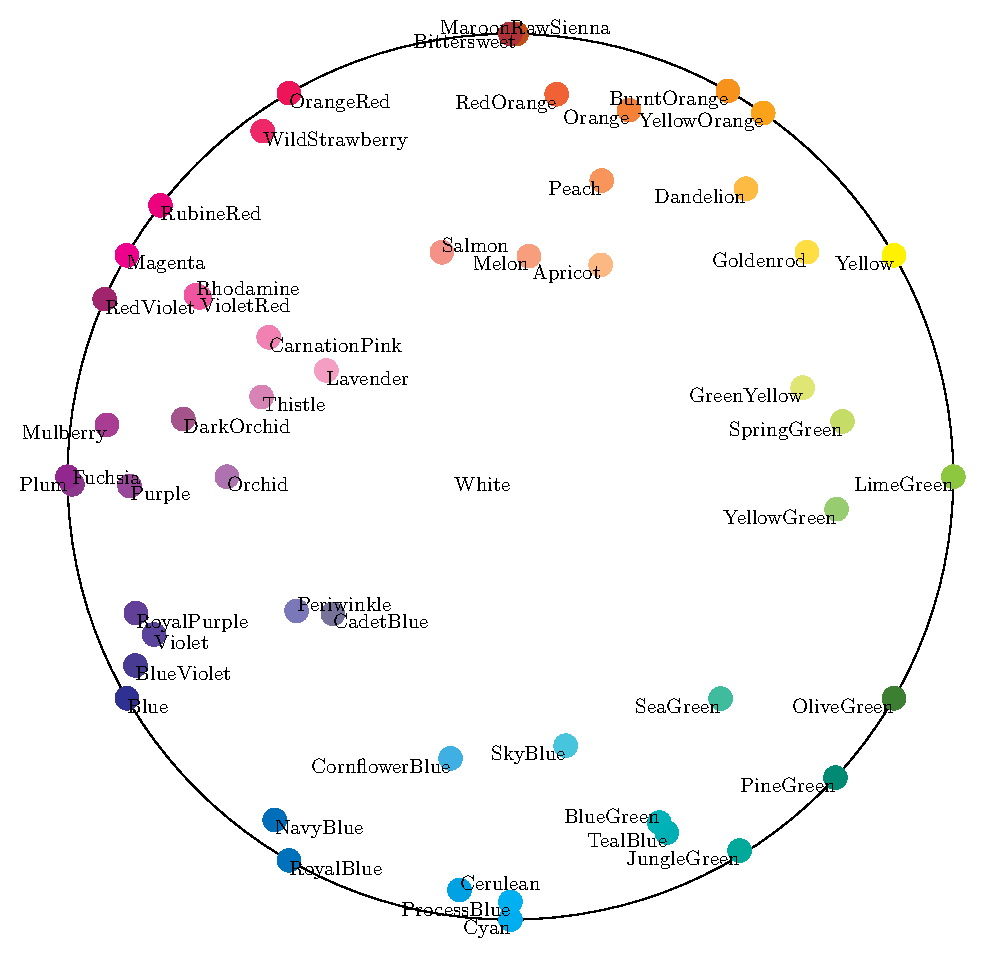
\includegraphics[width=\textwidth]{figures/pyx_colours.eps}
\end{center}
\caption[The named colours which PyXPlot recognises, arranged in HSB colour space]
{The named colours which PyXPlot recognises, arranged in HSB colour space, with the brightness axis orientated into the page. Some colours are not shown as they lie too close to others.}
\label{fig:colour_table3}
\end{figure}


% LINESTYLES.TEX
%
% The documentation in this file is part of PyXPlot
% <http://www.pyxplot.org.uk>
%
% Copyright (C) 2006-8 Dominic Ford <coders@pyxplot.org.uk>
%               2008   Ross Church
%
% $Id$
%
% PyXPlot is free software; you can redistribute it and/or modify it under the
% terms of the GNU General Public License as published by the Free Software
% Foundation; either version 2 of the License, or (at your option) any later
% version.
%
% You should have received a copy of the GNU General Public License along with
% PyXPlot; if not, write to the Free Software Foundation, Inc., 51 Franklin
% Street, Fifth Floor, Boston, MA  02110-1301, USA

% ----------------------------------------------------------------------------

% LaTeX source for the PyXPlot Users' Guide

\chapter{Line and Point Types}
\label{linetypes_table}

The table below shows the appearance of each numbered line and point type:

\noindent
\includegraphics[width=\textwidth]{examples/eps/ex_linestyles.eps}


% OTHER_APPS.TEX
%
% The documentation in this file is part of PyXPlot
% <http://www.pyxplot.org.uk>
%
% Copyright (C) 2006-7 Dominic Ford <coders@pyxplot.org.uk>
%               2008   Ross Church
%
% $Id$
%
% PyXPlot is free software; you can redistribute it and/or modify it under the
% terms of the GNU General Public License as published by the Free Software
% Foundation; either version 2 of the License, or (at your option) any later
% version.
%
% You should have received a copy of the GNU General Public License along with
% PyXPlot; if not, write to the Free Software Foundation, Inc., 51 Franklin
% Street, Fifth Floor, Boston, MA  02110-1301, USA

% ----------------------------------------------------------------------------

% LaTeX source for the PyXPlot Users' Guide

\chapter{Other Applications of PyXPlot}

In this chapter, we present a short cookbook, describing a few applications
which we have found for PyXPlot which are not directly related to the plotting
of graphs.

\section{Conversion of JPEG Images to Postscript}
\index{jpeg images}

Users of the \LaTeX\ typesetting system will have experienced frustration if
they have ever tried to incorporate bitmap images -- for example, those in jpeg
format -- into \LaTeX\ documents. Whilst \LaTeX's {\tt includegraphics} command
allows for the easy incorporation of encapsulated postscript images into
documents, bitmap images must be converted into postscript before they can be
imported. ImageMagick\index{ImageMagick}'s {\tt convert} command can perform
such a conversion, but it does not produce efficient postscript, and the
resulting postscript file sizes are often excessively large. PyXPlot's
\indcmdt{jpeg} can perform much more efficient conversion:

\begin{verbatim}
set output image.eps
jpeg 'image.jpg' width 10
\end{verbatim}

\section{Inserting Equations in Powerpoint Presentations}
\index{Microsoft Powerpoint}\index{presentations}

The two tools most commonly used for presenting talks\index{presentations} --
Microsoft {\it Powerpoint}\index{Microsoft Powerpoint} and
OpenOffice\index{OpenOffice} {\it Impress} -- have no facility for importing
text rendered in \LaTeX\ into slides. This is a frustration for those who work
in mathematical disciplines, where it is necessary for talks to include
equations. More generally, it is a frustration for anyone who works in a field
with notation which makes use of non-standard characters. {\it Powerpoint} does
include its own {\it Equation Editor}, but its output is considerably less
professional than that produced by \LaTeX.

It is possible to import graphic images into {\it Powerpoint}, but it cannot
read images in postscript format, the format in which \LaTeX\ produces its
output.

PyXPlot's {\tt gif} and {\tt png} terminals provide a fix for this problem, as
the following example demonstrates:

\begin{verbatim}
set term transparent noantialias gif ; set dpi 300
set output 'equation.gif' ; set multiplot

# Render the Planck blackbody formula in LaTeX
set textcolour yellow
text '$B_\nu = \frac{8\pi h}{c^3} \
\frac{\nu^3}{\exp \left( h\nu / kT \right) -1 }$' at 0,0
text 'The Planck Blackbody Formula:' at 0 , 0.75
\end{verbatim}

The result is a {\tt gif} image of the desired equation, with yellow text on a
transparent background. This can readily be imported into {\it Powerpoint} and
re-scaled to the desired size.

\section{Delivering Talks in PyXPlot}

Going one step further, PyXPlot can be used as a stand-alone tool for designing
slides for talks; it has several advantages over other presentation tools.  All
of the text which is placed on slides is rendered neatly in \LaTeX.  Images can
be placed on slides using the \indcmdts{jpeg} and \indcmdts{eps} commands, and
placed at any arbitrary co-ordinate position on the slide.  In comparison with
programs such as Microsoft {\it Powerpoint}\index{Microsoft Powerpoint} and
OpenOffice\index{OpenOffice} {\it Impress}, the text looks much neater,
especially if equations or unusual characters are required. In comparison with
\TeX-based programs such as Foil\TeX, it is much easier to incorporate images
around text to create colourful slides which will keep an audience attentive.

As an additional advantage, graphs can be plotted within the scripts describing
each slide, directly from \datafile s in your local filesystem. If you receive
new data shortly before giving a talk, it is a simple matter to re-run the
PyXPlot scripts and your slides will automatically pick up the new \datafile s.

Below, we outline our recipe for designing slides in PyXPlot. There are many
steps, but they do not take much time; many simply involve pasting text into
various files. Readers of the printed version of the manual may find it easier
to copy these files from the HTML version of this manual on the PyXPlot
website.

\subsection{Setting up Infrastructure}

First, a bit of infrastructure needs to be set up. Note that once this has been
done for one talk, the infrastructure can be copied directly from a previous
talk.

\begin{enumerate}
\item Make a new directory in which to put your talk:
\begin{verbatim}
mkdir my_talk
cd my_talk
\end{verbatim}
\item Make a directory into which you will put the PyXPlot scripts for your
individual slides:
\begin{verbatim}
mkdir scripts
\end{verbatim}
\item Make a directory into which you will put any graphic images which you
want to put into your talk to make it look pretty:
\begin{verbatim}
mkdir images
\end{verbatim}
\item Make a directory into which PyXPlot will put graphic images of your
slides:
\begin{verbatim}
mkdir slides
\end{verbatim}
\item Design a background for your slides. Open a paint program such as the
{\tt gimp}, create a new image which measures $1024\times768$\,pixels, and fill
it with colour. My preference tends to be for a blue colour gradient, running
from bright blue at the top to dark blue at the bottom, but you may be more
inventive than me. You may wish to add institutional and/or project logos in
the corners. Alternatively, you can download a ready-made background image from
the PyXPlot website: \url{http://foo}. You should store this image as {\tt
images/background.jpg}.
\item We need a simple PyXPlot script to set up a slide template. Paste the
following text into the file {\tt scripts/slide\_init}; there's a bit of black
magic in the {\tt arrow} commands in this script which it isn't necessary to
understand at this stage:\label{presentation_magic}
\begin{verbatim}
scale  = 1.25        ; inch = 2.54 # cm
width  = 10.24*scale ; height =  7.68*scale
x = width/100.0      ; y = height/100.0
set term gif ; set dpi (1024.0/width) * inch
set multiplot ; set nodisplay
set texthalign centre ; set textvalign centre
set textcolour yellow
jpeg "images/background.jpg" width width
arrow -x* 25,-y* 25 to -x* 25, y*125 with nohead
arrow -x* 25, y*125 to  x*125, y*125 with nohead
arrow  x*125, y*125 to  x*125,-y* 25 with nohead
arrow  x*125,-y* 25 to -x* 25,-y* 25 with nohead
\end{verbatim}
\item We also need a simple PyXPlot script to round off each slide. Paste the
following text into the file {\tt scripts/slide\_finish}:
\begin{verbatim}
set display ; refresh
\end{verbatim}
\item Paste the following text into the file {\tt compile}. This is a simple
shell script which instructs {\tt pyxplot\_watch} to compile your slides using
PyXPlot every time you edit any of the them:
\begin{verbatim}
#!/bin/bash
pyxplot_watch --verbose scripts/0\*
\end{verbatim}
\item Paste the following text into the file {\tt make\_slides}. This is a
simple shell script which crops your slides to measure exactly
$1024\times768$\,pixels, cropping any text boxes which may go off the side of
them. It links up with the black magic of Step~\ref{presentation_magic}:
\begin{verbatim}
#!/bin/bash
mkdir -p slides_cropped
for all in slides/*.gif ; do
convert $all -crop 1024x768+261+198 `echo $all | \
sed 's@slides@slides_cropped@' | sed 's@gif@jpg@'`
done
\end{verbatim}
\item Make the scripts {\tt compile} and {\tt make\_slides} executable:
\begin{verbatim}
chmod 755 compile make_slides
\end{verbatim}
\end{enumerate}

\subsection{Writing A Short Example Talk} 

The infrastructure is now completely set up, and you are ready to start
designing slides. As an example, we will now design a short talk which might be
presented to by the Principal Conductor of the {\it International Feline
Chamber Chorus}.

\begin{enumerate}
\item Run the script {\tt compile} and leave it running in the background.
PyXPlot will then re-run the scripts describing your slides whenever you edit
them.
\item As an example, we will now make a title slide. Paste the following script
into the file {\tt scripts/0001}:
\begin{verbatim}
set output 'slides/0001.gif'
load 'scripts/slide_init'

text '\parbox[t]{10cm}{\center \LARGE \bf \
  An Experiment in the Training \\ \
  of Cats to Sing Bach Chorales \
} ' at x*50, y*75
text '\Large \bf Sir Archibald Dribbles' at x*50, y*45
text '\parbox[t]{9cm}{\center \
  Principal Conductor, \\ \
  International Feline Chamber Chorus \
} ' at x*50, y*38
text 'Annual Lecture, 1st January 2008' at x*50, y*22

load 'scripts/slide_finish'
\end{verbatim}
Note that the variables {\tt x} and {\tt y} are defined to be 1~per cent of the
width and height of your slides respectively, such that the bottom-left of each
slide is at $(0,0)$ and the top-right of each slide is at $({\tt 100*x},{\tt
100*y})$.
\item Next we will make a second slide with a series of bullet points. Paste
the following script into the file {\tt scripts/0002}:
\begin{verbatim}
set output 'slides/0002.gif'
load 'scripts/slide_init'

text '\Large \textbf{Talk Overview}' at x*50, y*92
text "\parbox[t]{9cm}{\begin{itemize} \
 \item Teaching cats to use their head voices. \
 \item The Suzuki Method, as adapted to cats. \
 \item Case Study I: {\it Wachet auf, das Katzenfutter \
                          ist angerichtet!}, BWV~140. \
 \item Rhythmical Devices: Synchronised Purring. \
 \item Case Study II: {\it Was eine Katze will, das \
                           g'scheh' allzeit}, BWV~92. \
 \item Conclusion. \
 \end{itemize} \
} " at x*50 , y*60

set textcol cyan
text '{\bf With thanks to my collaborator, \
           Pebbles Poofslop.}' at x*50,y*15

load 'scripts/slide_finish'
\end{verbatim}
\item Finally, we will make a third slide with a graph on it. Paste the
following script into the file {\tt scripts/0003}:
\begin{verbatim}
set output 'slides/0003.gif'
load 'scripts/slide_init'

text '\Large \bf The Results of Our Model' at x*50, y*92
set axescolour yellow ; set nogrid
set origin x*17.5, y*20 ; set width x*70
set xrange [0.01:0.7]
set xlabel '$x$'
set yrange [0.01:0.7]
set ylabel '$f(x)$'
set palette Red, Green, Orange, Purple

set key top left
plot x t 'Model 1', exp(x)-1 t 'Model 2', \
     log(x+1) t 'Model 3', sin(x) t 'Model 4'

load 'scripts/slide_finish'
\end{verbatim}
\item To view your slides, run the script {\tt make\_slides}. Afterwards, you
will find your slides as a series of $1024\times768$\,pixel jpeg images in the
directory {\tt slides\_cropped}.  If you have the {\it Quick Image
Viewer}\index{Quick Image Viewer} ({\tt qiv}) installed, then you can view them
as follows:
\begin{verbatim}
qiv slides_cropped/*
\end{verbatim}
If you're in a hurry, you can skip the step of running the script {\tt
make\_slides} and view your slides as images in the {\tt slides} directory, but
note that the slides in here may not be properly cropped. This approach is
generally preferable when viewing your slides in a semi-live fashion as you are
editting them.
\item If you'd like to make the text on your slides larger or smaller, you can
do so by varying the {\tt scale} parameter in the file {\tt
scripts/slide\_init}.
\end{enumerate}

The three slides which we have designed can been seen in
Figures~\ref{presentation_slide1}, \ref{presentation_slide2} and
\ref{presentation_slide3}.

\subsection{Delivering your Talk}

There are two straightforward ways in which you can give your talk. The
quickest way is simply to use the {\it Quick Image Viewer}\index{Quick Image
Viewer} ({\tt qiv}):
\begin{verbatim}
qiv slides_cropped/*
\end{verbatim}
Press the left mouse button to move forward through your talk, and the right
mouse button to go back a slide.

This method does lack some of the niceties of Microsoft {\it Powerpoint} -- for
example, the ability to jump to any arbitrary slide number, compatibility with
wireless remote controls to advance your slides, and the ability to use
animated slide transitions. It may be preferably, therefore, to paste the jpeg
images of your slides into a {\it Powerpoint} or OpenOffice {\it Impress}
presentation before you give your talk.


% FIT_MATHS.TEX
%
% The documentation in this file is part of PyXPlot
% <http://www.pyxplot.org.uk>
%
% Copyright (C) 2006-9 Dominic Ford <coders@pyxplot.org.uk>
%               2008-9 Ross Church
%
% $Id$
%
% PyXPlot is free software; you can redistribute it and/or modify it under the
% terms of the GNU General Public License as published by the Free Software
% Foundation; either version 2 of the License, or (at your option) any later
% version.
%
% You should have received a copy of the GNU General Public License along with
% PyXPlot; if not, write to the Free Software Foundation, Inc., 51 Franklin
% Street, Fifth Floor, Boston, MA  02110-1301, USA

% ----------------------------------------------------------------------------

% LaTeX source for the PyXPlot Users' Guide

\chapter{The {\tt fit} Command: Mathematical Details}
\chaptermark{Details of the {\tt fit} command}
\label{fit_math}

In this section, the mathematical details of the workings of the \indcmdt{fit}
are described. This may be of interest in diagnosing its limitations, and also
in understanding the various quantities that it outputs after a fit is found.
This discussion must necessarily be a rather brief treatment of a large
subject; for a fuller account, the reader is referred to D.S.\ Sivia's {\it
Data Analysis: A Bayesian Tutorial}.

\section{Notation}
\label{bayes_notation}

I shall assume that we have some function $f()$, which takes $n_\mathrm{x}$
parameters, $x_0$...$x_{n_\mathrm{x}-1}$, the set of which may collectively be
written as the vector $\mathbf{x}$. We are supplied a datafile, containing a
number $n_\mathrm{d}$ of datapoints, each consisting of a set of values for
each of the $n_\mathrm{x}$ parameters, and one for the value which we are
seeking to make $f(\mathbf{x})$ match. I shall call of parameter values for the
$i$th datapoint $\mathbf{x}_i$, and the corresponding value which we are trying
to match $f_i$. The datafile may contain error estimates for the values $f_i$,
which I shall denote $\sigma_i$. If these are not supplied, then I shall
consider these quantities to be unknown, and equal to some constant
$\sigma_\mathrm{data}$.

Finally, I assume that there are $n_\mathrm{u}$ coefficients within the
function $f()$ that we are able to vary, corresponding to those variable names
listed after the {\tt via} statement in the {\tt fit} command. I shall
call these coefficients $u_0$...$u_{n_\mathrm{u}-1}$, and refer to them
collectively as $\mathbf{u}$.

I model the values $f_i$ in the supplied datafile as being noisy
Gaussian-distributed observations of the true function $f()$, and within this
framework, seek to find that vector of values $\mathbf{u}$ which is most
probable, given these observations. The probability of any given $\mathbf{u}$
is written
$\mathrm{P}\left( \mathbf{u} | \left\{ \mathbf{x}_i, f_i, \sigma_i \right\} \right)$.

\section{The Probability Density Function}
\label{bayes_pdf}

Bayes' Theorem states that:

\begin{equation}
\mathrm{P}\left( \mathbf{u} | \left\{ \mathbf{x}_i, f_i, \sigma_i \right\} \right) =
\frac{
\mathrm{P}\left( \left\{f_i \right\} | \mathbf{u}, \left\{ \mathbf{x}_i, \sigma_i \right\} \right)
\mathrm{P}\left( \mathbf{u} | \left\{ \mathbf{x}_i, \sigma_i \right\} \right)
}{
\mathrm{P}\left( \left\{f_i \right\} | \left\{ \mathbf{x}_i, \sigma_i \right\} \right)
}
\end{equation}

Since we are only seeking to maximise the quantity on the left, and the
denominator, termed the Bayesian \textit{evidence}, is independent of
$\mathbf{u}$, we can neglect it and replace the equality sign with a
proportionality sign.  Furthermore, if we assume a uniform prior, that is, we
assume that we have no prior knowledge to bias us towards certain more favoured
values of $\mathbf{u}$, then $\mathrm{P}\left( \mathbf{u} \right)$ is also a
constant which can be neglected. We conclude that maximising $\mathrm{P}\left(
\mathbf{u} | \left\{ \mathbf{x}_i, f_i, \sigma_i \right\} \right)$ is
equivalent to maximising $\mathrm{P}\left( \left\{f_i \right\} | \mathbf{u},
\left\{ \mathbf{x}_i, \sigma_i \right\} \right)$.

Since we are assuming $f_i$ to be Gaussian-distributed observations of the true
function $f()$, this latter probability can be written as a product of
$n_\mathrm{d}$ Gaussian distributions:

\begin{equation}
\mathrm{P}\left( \left\{f_i \right\} | \mathbf{u}, \left\{ \mathbf{x}_i, \sigma_i \right\} \right)
=
\prod_{i=0}^{n_\mathrm{d}-1} \frac{1}{\sigma_i\sqrt{2\pi}} \exp \left(
\frac{
-\left[f_i - f_\mathbf{u}(\mathbf{x}_i)\right]^2
}{
2 \sigma_i^2
} \right)
\end{equation}

The product in this equation can be converted into a more computationally
workable sum by taking the logarithm of both sides. Since logarithms are
monotonically increasing functions, maximising a probability is equivalent to
maximising its logarithm. We may write the logarithm $L$ of $\mathrm{P}\left(
\mathbf{u} | \left\{ \mathbf{x}_i, f_i, \sigma_i \right\} \right)$ as:

\begin{equation}
L = \sum_{i=0}^{n_\mathrm{d}-1}
\left( \frac{
-\left[f_i - f_\mathbf{u}(\mathbf{x}_i)\right]^2
}{
2 \sigma_i^2
} \right) + k
\end{equation}

\noindent where $k$ is some constant which does not affect the maximisation
process. It is this quantity, the familiar sum-of-square-residuals, that we
numerically maximise to find our best-fitting set of parameters, which I shall
refer to from here on as $\mathbf{u}^0$.

\section{Estimating the Error in $\mathbf{u}^0$}

To estimate the error in the best-fitting parameter values that we find, we
assume $\mathrm{P}\left( \mathbf{u} | \left\{ \mathbf{x}_i, f_i, \sigma_i
\right\} \right)$ to be approximated by an $n_\mathrm{u}$-dimensional Gaussian
distribution around $\mathbf{u}^0$. Taking a Taylor expansion of
$L(\mathbf{u})$ about $\mathbf{u}^0$, we can write:

\begin{eqnarray}
L(\mathbf{u}) & = & L(\mathbf{u}^0) +
    \underbrace{
      \sum_{i=0}^{n_\mathrm{u}-1} \left( u_i - u^0_i \right)
      \left.\frac{\partial L}{\partial u_i}\right|_{\mathbf{u}^0}
    }_{\textrm{Zero at $\mathbf{u}^0$ by definition}} + \label{L_taylor_expand}\\
& & \sum_{i=0}^{n_\mathrm{u}-1} \sum_{j=0}^{n_\mathrm{u}-1} \frac{\left( u_i - u^0_i \right) \left( u_j - u^0_j \right)}{2}
    \left.\frac{\partial^2 L}{\partial u_i \partial u_j}\right|_{\mathbf{u}^0} +
    \mathcal{O}\left( \mathbf{u} - \mathbf{u}^0\right)^3 \nonumber
\end{eqnarray}

Since the logarithm of a Gaussian distribution is a parabola, the quadratic
terms in the above expansion encode the Gaussian component of the probability
distribution $\mathrm{P}\left( \mathbf{u} | \left\{ \mathbf{x}_i, f_i, \sigma_i
\right\} \right)$ about $\mathbf{u}^0$.\footnote{The use of this is called
\textit{Gauss' Method}. Higher order terms in the expansion represent any
non-Gaussianity in the probability distribution, which we neglect. See MacKay,
D.J.C., \textit{Information Theory, Inference and Learning Algorithms}, CUP
(2003).} We may write the sum of these terms, which we denote $Q$, in matrix
form:

\begin{equation}
Q = \frac{1}{2} \left(\mathbf{u} - \mathbf{u}^0\right)^\mathbf{T} \mathbf{A} \left(\mathbf{u} - \mathbf{u}^0\right)
\label{Q_vector}
\end{equation}

\noindent where the superscript $^\mathbf{T}$ represents the transpose of the
vector displacement from $\mathbf{u}^0$, and $\mathbf{A}$ is the Hessian matrix
of $L$, given by:

\begin{equation}
A_{ij} = \nabla\nabla L = \left.\frac{\partial^2 L}{\partial u_i \partial u_j}\right|_{\mathbf{u}^0}
\end{equation}
\index{Hessian matrix}

This is the Hessian matrix which is output by the {\tt fit} command. In
general, an $n_\mathrm{u}$-dimensional Gaussian distribution such as that given
by equation~(\ref{L_taylor_expand}) yields elliptical contours of
equiprobability in parameter space, whose principal axes need not be aligned
with our chosen co-ordinate axes -- the variables $u_0 ... u_{n_u-1}$. The
eigenvectors $\mathbf{e}_i$ of $\mathbf{A}$ are the principal axes of these
ellipses, and the corresponding eigenvalues $\lambda_i$ equal $1/\sigma_i^2$,
where $\sigma_i$ is the standard deviation of the probability density function
along the direction of these axes.

This can be visualised by imagining that we diagonalise $\mathbf{A}$, and
expand equation~(\ref{Q_vector}) in our diagonal basis. The resulting
expression for $L$ is a sum of square terms; the cross terms vanish in this
basis by definition. The equations of the equiprobability contours become the
equations of ellipses:

\begin{equation}
Q = \frac{1}{2} \sum_{i=0}^{n_\mathrm{u}-1} A_{ii} \left(u_i - u^0_i\right)^2 = k
\end{equation}

\noindent where $k$ is some constant. By comparison with the equation for the
logarithm of a Gaussian distribution, we can associate $A_{ii}$ with
$-1/\sigma_i^2$ in our eigenvector basis.

The problem of evaluating the standard deviations of our variables $u_i$ is
more complicated, however, as we are attempting to evaluate the width of these
elliptical equiprobability contours in directions which are, in general, not
aligned with their principal axes. To achieve this, we first convert our
Hessian matrix into a covariance matrix.

\section{The Covariance Matrix}
\index{covariance matrix}

The terms of the covariance matrix $V_{ij}$ are defined by:

\begin{equation}
\label{def_covar}
V_{ij} = \left< \left(u_i - u^0_i\right) \left(u_j - u^0_j\right) \right>
\end{equation}

\noindent Its leading diagonal terms may be recognised as equalling the
variances of each of our $n_\mathrm{u}$ variables; its cross terms measure the
correlation between the variables. If a component $V_{ij} > 0$, it implies that
higher estimates of the coefficient $u_i$ make higher estimates of $u_j$ more
favourable also; if $V_{ij} < 0$, the converse is true.

It is a standard statistical result that $\mathbf{V} = (-\mathbf{A})^{-1}$. In
the remainder of this section we prove this; readers who are willing to accept
this may skip onto Section~\ref{correlation_matrix}.

Using $\Delta u_i$ to denote $\left(u_i - u^0_i\right)$, we may proceed by
rewriting equation~(\ref{def_covar}) as:

\begin{eqnarray}
V_{ij} & = & \idotsint_{u_i=-\infty}^{\infty}
\Delta u_i \Delta u_j
\mathrm{P}\left(
\mathbf{u} | \left\{ \mathbf{x}_i, f_i, \sigma_i \right\} \right)
\,\mathrm{d}^{n_\mathrm{u}}\mathbf{u} \\
 & = & \frac{
\idotsint_{u_i=-\infty}^{\infty} \Delta u_i \Delta u_j \exp(-Q) \,\mathrm{d}^{n_\mathrm{u}}\mathbf{u}
}{
\idotsint_{u_i=-\infty}^{\infty} \exp(-Q) \,\mathrm{d}^{n_\mathrm{u}}\mathbf{u}
}
\nonumber
\end{eqnarray}

The normalisation factor in the denominator of this expression, which we denote
as $Z$, the \textit{partition function}, may be evaluated by
$n_\mathrm{u}$-dimensional Gaussian integration, and is a standard result:

\begin{eqnarray}
Z & = & \idotsint_{u_i=-\infty}^{\infty} \exp\left(\frac{1}{2} \Delta \mathbf{u}^\mathbf{T} \mathbf{A} \Delta \mathbf{u} \right) \,\mathrm{d}^{n_\mathrm{u}}\mathbf{u} \\
& = & \frac{(2\pi)^{n_\mathrm{u}/2}}{\mathrm{Det}(\mathbf{-A})} \nonumber
\end{eqnarray}

Differentiating $\log_e(Z)$ with respect of any given component of the Hessian
matrix $A_{ij}$ yields:

\begin{equation}
-2 \frac{\partial}{\partial A_{ij}} \left[ \log_e(Z) \right] = \frac{1}{Z}
\idotsint_{u_i=-\infty}^{\infty} \Delta u_i \Delta u_j \exp(-Q) \,\mathrm{d}^{n_\mathrm{u}}\mathbf{u}
\end{equation}

\noindent which we may identify as equalling $V_{ij}$:

\begin{eqnarray}
\label{v_zrelate}
V_{ij} & = & -2 \frac{\partial}{\partial A_{ij}} \left[ \log_e(Z) \right] \\
& = & -2 \frac{\partial}{\partial A_{ij}} \left[ \log_e((2\pi)^{n_\mathrm{u}/2}) - \log_e(\mathrm{Det}(\mathbf{-A})) \right] \nonumber \\
& = & 2 \frac{\partial}{\partial A_{ij}} \left[ \log_e(\mathrm{Det}(\mathbf{-A})) \right] \nonumber
\end{eqnarray}

\noindent This expression may be simplified by recalling that the determinant
of a matrix is equal to the scalar product of any of its rows with its
cofactors, yielding the result:

\begin{equation}
\frac{\partial}{\partial A_{ij}} \left[\mathrm{Det}(\mathbf{-A})\right] = -a_{ij}
\end{equation}

\noindent where $a_{ij}$ is the cofactor of $A_{ij}$. Substituting this into
equation~(\ref{v_zrelate}) yields:

\begin{equation}
V_{ij} = \frac{-a_{ij}}{\mathrm{Det}(\mathbf{-A})}
\end{equation}

Recalling that the adjoint $\mathbf{A}^\dagger$ of the Hessian matrix is the
matrix of cofactors of its transpose, and that $\mathbf{A}$ is symmetric, we
may write:

\begin{equation}
V_{ij} = \frac{-\mathbf{A}^\dagger}{\mathrm{Det}(\mathbf{-A})} \equiv (-\mathbf{A})^{-1}
\end{equation}

\noindent which proves the result stated earlier.

\section{The Correlation Matrix}
\label{correlation_matrix}
\index{correlation matrix}

Having evaluated the covariance matrix, we may straightforwardly find the
standard deviations in each of our variables, by taking the square roots of the
terms along its leading diagonal. For datafiles where the user does not specify
the standard deviations $\sigma_i$ in each value $f_i$, the task is not quite
complete, as the Hessian matrix depends critically upon these uncertainties,
even if they are assumed the same for all of our $f_i$. This point is returned
to in Section~\ref{finding_sigmai}.

The correlation matrix $\mathbf{C}$, whose terms are given by:

\begin{equation}
C_{ij} = \frac{V_{ij}}{\sigma_i\sigma_j}
\end{equation}

\noindent may be considered a more user-friendly version of the covariance
matrix for inspecting the correlation between parameters. The leading diagonal
terms are all clearly equal unity by construction. The cross terms lie in the
range $-1 \leq C_{ij} \leq 1$, the upper limit of this range representing
perfect correlation between parameters, and the lower limit perfect
anti-correlation.

\section{Finding $\sigma_i$}
\label{finding_sigmai}

Throughout the preceding sections, the uncertainties in the supplied target
values $f_i$ have been denoted $\sigma_i$ (see Section~\ref{bayes_notation}).
The user has the option of supplying these in the source datafile, in which
case the provisions of the previous sections are now complete; both
best-estimate parameter values and their uncertainties can be calculated. The
user may also, however, leave the uncertainties in $f_i$ unstated, in which
case, as described in Section~\ref{bayes_notation}, we assume all of the data
values to have a common uncertainty $\sigma_\mathrm{data}$, which is an
unknown.

In this case, where $\sigma_i = \sigma_\mathrm{data} \,\forall\, i$, the best
fitting parameter values are independent of $\sigma_\mathrm{data}$, but the
same is not true of the uncertainties in these values, as the terms of the
Hessian matrix do depend upon $\sigma_\mathrm{data}$. We must therefore
undertake a further calculation to find the most probable value of
$\sigma_\mathrm{data}$, given the data. This is achieved by maximising
$\mathrm{P}\left( \sigma_\mathrm{data} | \left\{ \mathbf{x}_i, f_i \right\}
\right)$. Returning once again to Bayes' Theorem, we can write:

\begin{equation}
\mathrm{P}\left( \sigma_\mathrm{data} | \left\{ \mathbf{x}_i, f_i \right\} \right)
= \frac{
\mathrm{P}\left( \left\{ f_i \right\} | \sigma_\mathrm{data}, \left\{ \mathbf{x}_i \right\} \right)
\mathrm{P}\left( \sigma_\mathrm{data} | \left\{ \mathbf{x}_i \right\} \right)
}{
\mathrm{P}\left( \left\{ f_i \right\} | \left\{ \mathbf{x}_i \right\} \right)
}
\end{equation}

As before, we neglect the denominator, which has no effect upon the
maximisation problem, and assume a uniform prior $\mathrm{P}\left(
\sigma_\mathrm{data} | \left\{ \mathbf{x}_i \right\} \right)$. This reduces the
problem to the maximisation of $\mathrm{P}\left( \left\{ f_i \right\} |
\sigma_\mathrm{data}, \left\{ \mathbf{x}_i \right\} \right)$, which we may
write as a marginalised probability distribution over $\mathbf{u}$:

\begin{eqnarray}
\label{p_f_given_sigma}
\mathrm{P}\left( \left\{ f_i \right\} | \sigma_\mathrm{data}, \left\{ \mathbf{x}_i \right\} \right) =
\idotsint_{-\infty}^{\infty}
&
\mathrm{P}\left( \left\{ f_i \right\} | \sigma_\mathrm{data}, \left\{ \mathbf{x}_i \right\}, \mathbf{u} \right)
\times & \\ &
\mathrm{P}\left( \mathbf{u} | \sigma_\mathrm{data}, \left\{ \mathbf{x}_i \right\} \right)
\,\mathrm{d}^{n_\mathrm{u}}\mathbf{u}
& \nonumber
\end{eqnarray}

Assuming a uniform prior for $\mathbf{u}$, we may neglect the latter term in
the integral, but even with this assumption, the integral is not generally
tractable, as $\mathrm{P}\left( \left\{ f_i \right\} | \sigma_\mathrm{data},
\left\{ \mathbf{x}_i \right\}, \left\{ \mathbf{u}_i \right\} \right)$ may well
be multimodal in form. However, if we neglect such possibilities, and assume
this probability distribution to be approximate a Gaussian \textit{globally},
we can make use of the standard result for an $n_\mathrm{u}$-dimensional Gaussian integral:

\begin{equation}
\idotsint_{-\infty}^{\infty}
\exp \left(
\frac{1}{2}\mathbf{u}^\mathbf{T} \mathbf{A} \mathbf{u}
\right) \,\mathrm{d}^{n_\mathrm{u}}\mathbf{u}
=
\frac{
(2\pi)^{n_\mathrm{u}/2}
}{
\sqrt{\mathrm{Det}\left(-\mathbf{A}\right)}
}
\end{equation}

\noindent We may thus approximate equation~(\ref{p_f_given_sigma}) as:

\begin{eqnarray}
\mathrm{P}\left( \left\{ f_i \right\} | \sigma_\mathrm{data}, \left\{ \mathbf{x}_i \right\} \right)
& \approx &
\mathrm{P}\left( \left\{ f_i \right\} | \sigma_\mathrm{data}, \left\{ \mathbf{x}_i \right\}, \mathbf{u}^0 \right)
\times \\
& &
\mathrm{P}\left( \mathbf{u}^0 | \sigma_\mathrm{data}, \left\{ \mathbf{x}_i, f_i \right\} \right)
\frac{
(2\pi)^{n_\mathrm{u}/2}
}{
\sqrt{\mathrm{Det}\left(-\mathbf{A}\right)}
}
\nonumber
\end{eqnarray}

As in Section~\ref{bayes_pdf}, it is numerically easier to maximise this
quantity via its logarithm, which we denote $L_2$, and can write as:

\begin{eqnarray}
L_2 & = &
\sum_{i=0}^{n_\mathrm{d}-1}
\left(
\frac{
-\left[f_i - f_{\mathbf{u}^0}(\mathbf{x}_i)\right]^2
}{
2\sigma_\mathrm{data}^2
}
- \log_e \left(2\pi\sqrt{\sigma_\mathrm{data}} \right)
\right) +
\\ & & \nonumber
\log_e \left(
\frac{
(2\pi)^{n_\mathrm{u}/2}
}{
\sqrt{\mathrm{Det}\left(-\mathbf{A}\right)}
}
\right)
\end{eqnarray}

This quantity is maximised numerically, a process simplified by the fact that
$\mathbf{u}^0$ is independent of $\sigma_\mathrm{data}$.

% CHANGELOG.TEX
%
% The documentation in this file is part of PyXPlot
% <http://www.pyxplot.org.uk>
%
% Copyright (C) 2006-7 Dominic Ford <coders@pyxplot.org.uk>
%               2008   Ross Church
%
% $Id$
%
% PyXPlot is free software; you can redistribute it and/or modify it under the
% terms of the GNU General Public License as published by the Free Software
% Foundation; either version 2 of the License, or (at your option) any later
% version.
%
% You should have received a copy of the GNU General Public License along with
% PyXPlot; if not, write to the Free Software Foundation, Inc., 51 Franklin
% Street, Fifth Floor, Boston, MA  02110-1301, USA

% ----------------------------------------------------------------------------

% LaTeX source for the PyXPlot Users' Guide

\chapter{ChangeLog}
\index{ChangeLog}

\subsection*{2008 Apr 19: PyXPlot 0.7.0}

\subsubsection*{Summary:}

Third PyXPlot beta-release. The code has undergone significant streamlining,
and now runs approximately twice as fast as version 0.6.3 when handling large
datafiles. Memory usage has also been radically reduced. Two new data
processing commands have been introduced. The {\tt tabulate} command can be
used to produce textual datafiles, allowing the user to read data in from
files, apply some analysis, and then write the processed data back to file. The
{\tt histogram} command can be used to estimate the frequency densities of sets
of data points, either by binning them into a bar chart, or by fitting a
functional form to their frequency density.

\subsubsection*{Details -- New and Extended Commands:}

\begin{itemize}
\item {\tt tabulate}
\item {\tt histogram}
\item {\tt set label} and {\tt text} commands extended to allow a colour to be
specified.
\end{itemize}

\subsubsection*{Details -- API changes}

\begin{itemize}
\item {\tt diff\_dx()} and {\tt int\_dx()} functions -- the function to be
differentiated or integrated must now be placed in quote marks.
\end{itemize}

\subsubsection*{Details -- Change of System Requirements:}

\begin{itemize}
\item Requirement of PyX version 0.9 updated to PyX version 0.10. Note that new versions of the PyX graphics library are not generally backwardly compatible.
\end{itemize}

\subsection*{2007 Feb 26: PyXPlot 0.6.3}

\subsubsection*{Summary:}

Second PyXPlot beta-release. The most significant change is the introduction of
a new command-line parser, with greatly improved handling of complex
expressions and much more meaningful syntax error messages. Multi-platform
compatibility has also been massively improved, and dependencies loosened.  A
small number of new commands have been added; most notable among them are the
{\tt jpeg} and {\tt eps} commands, which embed images in multiplots.

\subsubsection*{Details -- New and Extended Commands:}

\begin{itemize}
\item {\tt jpeg}
\item {\tt eps}
\item {\tt set xtics} and {\tt set mxtics}
\item {\tt text} and {\tt set label} commands extended to allow text rotation.
\item {\tt set log} command extended to allow the use of logarithms with bases other than 10.
\item {\tt set preamble}
\item {\tt set term enlarge | noenlarge}
\item {\tt set term pdf}
\item {\tt set term x11\_persist}
\end{itemize}

\subsubsection*{Details -- Eased System Requirements:}

\begin{itemize}
\item Requirement on Python 2.4 minimum eased to version 2.3 minimum.
\item Requirements on scipy and readline eased; PyXPlot will now work in reduced form when they are absent, though they are still strongly recommended.
\item dvips and ghostscript are no longer required.
\end{itemize}

\subsubsection*{Details -- Removed Commands:}

Due to a general refinement of PyXPlot's API, some of the less sensible pieces
of syntax from Version~0.5 are no longer supported. The author apologises for
any inconvenience caused.

\begin{itemize}
\item The {\tt delete\_arrow}, {\tt delete\_text}, {\tt move\_text}, {\tt undelete\_arrow} and {\tt undelete\_text} commands have been removed from the PyXPlot API. The {\tt move}, {\tt delete} and {\tt undelete} commands should now be used to act upon all types of multiplot objects.
\item The {\tt set terminal} command no longer accepts the {\tt enhanced} and {\tt noenhanced} modifiers. The {\tt postscript} and {\tt eps} terminals should be used instead.
\item The {\tt select} modifier, used after the {\tt plot}, {\tt replot}, {\tt fit} and {\tt spline} command can now only be used once; to specify multiple {\tt select} criteria, use the {\tt and} logical operator.
\end{itemize}

\subsection*{2006 Sep 09: PyXPlot 0.5.8}

First beta-release.


\printindex
\end{document}
